\documentclass[11pt,a4paper,openright]{amsbook}

%Fonts

\usepackage{libertine}
\usepackage{euler}
\usepackage[T1]{fontenc}

%Packages.

%\usepackage[parfill]{parskip}
\usepackage{verbatim}
\usepackage{amsmath}
\usepackage{amssymb}
%\usepackage{amsfonts}
\usepackage{amsthm}
\usepackage{mathrsfs}
\usepackage{tikz}
\usetikzlibrary{matrix,arrows}
\usepackage[all]{xy}
\usepackage{mathrsfs}
\usepackage{a4wide}
\usepackage{enumerate}
\usepackage{hyperref}
%\usepackage{showkeys}
\usepackage{setspace}
%\usepackage{fancyhdr}

%Theorem styles.

\theoremstyle{plain}
\newtheorem{conj}{Conjecture}
\newtheorem{theorem}{Theorem}%[section]
\newtheorem{lemma}[theorem]{Lemma}%[section]
\newtheorem{proposition}[theorem]{Proposition}%[section]
\newtheorem{corollary}[theorem]{Corollary}%[section]
\newtheorem{claim}[theorem]{Claim}%[section]
\newtheorem{question}[theorem]{Question}
\newtheorem{conjecture}[theorem]{Conjecture}
\newtheorem*{thm}{Theorem}

\theoremstyle{definition}%[section]
\newtheorem{definition}[theorem]{Definition}%[section]
\newtheorem{example}[theorem]{Example}%[section]
\newtheorem{project}{Project}

\theoremstyle{remark}%[section]
\newtheorem{remark}[theorem]{Remark}%[section]

%Numbering and contents

%\numberwithin{theorem}{section}
\setcounter{tocdepth}{5}
\setlength{\parindent}{0pt}
\setlength{\parskip}{1ex}

% Editting \Chapter

%Shorthand for hats.

\newcommand{\G}{\mathcal{G}}
\newcommand{\E}{\widehat{E}}
\newcommand{\X}{\widehat{X}}
\newcommand{\A}{\widehat{A}}

%Line Spacing
%\setstretch{1.6}

\newcommand{\ucong}{\rotatebox{90}{$\cong$}}
\newenvironment{chpt}{\newpage\normalfont\Large\bfseries \begin{center}}{\end{center}}
\title{Inverse Semigroups in Coarse Geometry.} 
\date{April 2013}
\author{Martin Finn-Sell}


\begin{document}
%\maketitle

\begin{titlepage}
\begin{center}

\huge University of Southampton \\[1cm]

\large Faculty of Social and Human Sciences \\[0.5cm]
\LARGE Mathematical Sciences \\[2cm]
\huge \textbf{Inverse Semigroups in Coarse Geometry} \\[2.5cm]

\Large Martin Finn-Sell\\[2cm]

\large A thesis submitted for for the degree of\\
Doctor of Philosophy\\[8cm]

\large May 2013

\end{center}
\end{titlepage}



\bibliographystyle{alpha}
%\setstretch{1.3}

\frontmatter
\begin{center}
UNIVERSITY OF SOUTHAMPTON\\[0.75cm]

\underline{ABSTRACT}\\[0.55cm]

FACULTY OF SOCIAL AND HUMAN SCIENCES\\
SCHOOL OF MATHEMATICS\\[0.75cm]

\underline{Doctor of Philosophy}\\[0.55cm]

INVERSE SEMIGROUPS IN COARSE GEOMETRY\\[0.6cm]

By Martin Finn-Sell\\[1.5cm]
\end{center}


\addcontentsline{toc}{chapter}{Abstract.}
Inverse semigroups provide a natural way to encode combinatorial data from geometric settings. Examples of this occur in both geometry and topology, where the data comes in the form of partial bijections that preserve the topology, and operator algebras, where the partial bijections encode $*$-subsemigroups of partial isometries of Hilbert space. In this thesis we explore the connections between these two pictures within the backdrop of coarse geometry.

The first collection of results are concerned primarily with inverse semigroups and their $C^{*}$-algebras. We give a construction of a six term sequence of $C^{*}$-algebras connecting the semigroup $C^{*}$-algebra to that of a naturally associated group $C^{*}$-algebra. This result is a generalisation of the ideas of Pimsner and Voiculescu, who were concerned with computing K-theory groups associated to actions of groups. We outline how to connect this picture, via groupoids, to that of a partial translation algebra of Brodzki, Niblo and Wright, and further consider applications of these sequences to computations of certain K-groups associated with group and semigroup $C^{*}$-algebras.

Secondly, we give an account of the coarse Baum-Connes conjecture associated to a uniformly discrete bounded geometry metric space and rephrase the conjecture in terms of groupoids and their $C^{*}$-algebras that can naturally be associated to a metric space. We then consider the well-known counterexamples to this conjecture, giving a unifying framework for their study in terms of groupoids and a new conjecture for metric spaces known as the boundary coarse Baum-Connes conjecture. We prove this conjecture, generalising a result of Willett and Yu, for certain classes of expanders including those of large girth by constructing a partial action of a discrete group on such spaces.


%
%\newpage
%\thispagestyle{empty}~
%\newpage
\addcontentsline{toc}{chapter}{Contents.}
\tableofcontents

\begin{chpt}Author's Declaration.\end{chpt}
\addcontentsline{toc}{chapter}{Author's Declaration.}
I, Martin Finn-Sell, declare that the thesis entitled \textit{Inverse Semigroups in Coarse Geometry} and the work presented in the thesis are both my own, and have been generated by me as the result of my own original research. I confirm that:
\begin{itemize}
\item this work was done wholly or mainly while in candidature for a research degree at this University;
\item where any part of this thesis has previously been submitted for a degree or any other qualification at this University or any other institution, this has been clearly stated;
\item where I have consulted the published work of others, this is always clearly attributed;
\item where I have quoted from the work of others, the source is always given. With the exception of such quotations, this thesis is entirely my own work;
\item I have acknowledged all main sources of help;
\item where the thesis is based on work done by myself jointly with others, I have made clear exactly what was done by others and what I have contributed myself;
\item parts of this work have been published, as a preprint: \textit{Spaces of Graphs, Boundary Groupoids and the Coarse Baum-Connes Conjecture}, Martin Finn-Sell and Nick Wright, 2012\\
URL: http://arxiv.org/abs/1208.4237
\end{itemize}
\bigskip
Signed ..............................................................................
Date ..............................................................................
\newpage
\begin{chpt}Acknowledgements.\end{chpt}
\addcontentsline{toc}{chapter}{Acknowledgements.}

\mainmatter
\setstretch{1.6}
\chapter{Introduction.}

General fluff about inverse semigroups and groupoids being important, particular examples include the partial action of a discrete group in both cases. Connect in the work on partial symmetries, remark that this connects work on tilings as well as work of Macbeth on decidablity problems for certain groups.

Outline the general approach we're going to use in the thesis. Move to some specific examples.

\subsection{The work of Pimsner and Voiculescu.}

This leads to certain generalisations associated to F-inverse monoids...

State the main results on this, and outline certain K-theory discussions. This is part 1; Using partial actions of a group to understand the group.

\subsection{Counterexamples to the coarse Baum-Connes conjecture.}

This arises from considering certain bad graphs. Explain why this conjecture is relevant, and why on earth understanding the graphs is a good idea. Explain that natural examples come with a group action, and explain that we generalise this idea to get bad sequences with a partial free group action. .

Outline the main theorems.

This is ii), understanding a space by understanding that it admits a partial group action.

\subsection{Further connections.}

Explain that the ideas arising from chapter 3 will connect with those of chapter 4. And outline how this connection runs through a partial translation structure / algebra. This is interplay between i) and ii)

State some results;

Explain the outgoing ideas and open problems this thesis leaves behind.

Smile. It's only 6-10 pages!


%\setstretch{1.6}
\chapter{The Basics.}
As outlined in the introduction inverse semigroups and groupoids play a large role in the development of many aspects of combinatorics, graph theory and analysis. In this section we provide some basics concerning these objects and the connections between them, developing the notion of Paterson and Exel of a \textit{universal groupoid} associated to an inverse semigroup. We then give a brief introduction to operator algebras, focusing on the situation that arises naturally from both inverse semigroups and groupoids. Lastly, we consider topological K-theory of $C^{*}$-algebras; we outline all the tools we need for the later chapters.

\section{Semigroup and Groupoid Theory.}

A \textit{semigroup} is a set $S$, together with an associative binary operation. If additionally it has a unit element, then we say it is a \textit{monoid}.

\begin{definition}\label{Def:invsemi}
Let $S$ be a semigroup. We say $S$ is $inverse$ if there exists a unary operation $*:S \rightarrow S$ satisfying the following identities:
\begin{enumerate}
\item $(s^{*})^{*}=s$
\item $ss^{*}s=s$ and $s^{*}ss^{*}=s^{*}$ for all $s \in S$
\item $ef=fe$ for all idempotents $e,f \in S$ 
\end{enumerate}
\end{definition}

A very fundamental example of such an object is the \textit{symmetric inverse monoid} on any set $X$; consider the collection of all partial bijections of $X$ to itself, giving them them the natural composition law associated to functions - that is find the largest possible domain on which the composition makes sense, shown below in Figure \ref{Fig:Comp}.


\begin{figure}[h]
\begin{center}

%Def of Circles needed
\def\firstcircle{(-0.25,-1.25) circle (1.0cm)}
\def\secondcircle{(-0.25,0) circle (1.0cm)}
\def\thirdcircle{(-4.75,0) circle (1.0cm)}
\def\forthcircle{(-4.75,-2.5) circle (1.0cm)}
\def\fifthcircle{(-4.75,-1.25) circle (1.0cm)}

\tikzset{filled/.style={fill=circle area, draw=circle edge, thick},
    outline/.style={draw=circle edge, thick}}
    
\setlength{\parskip}{5mm}
% Set A and B
\begin{tikzpicture}
    \begin{scope}[fill opacity=0.5]
        \clip \firstcircle
              \fifthcircle;
        \fill[filled] \secondcircle
                      \thirdcircle
                      \forthcircle;
        \end{scope}
               
    %\draw[outline]    
    \draw[outline] \firstcircle node [below] {$dom(f_{2})$};
    \draw[outline] \secondcircle node [above] {$im(f_{1})$};
    \draw[outline] \thirdcircle node [above] {$dom(f_{1})$};
    \draw[outline] \forthcircle node [below] {$im(f_{1})$};
        %\node[anchor=south] at (current bounding box.north) {$A \cap B$};
    \draw[>=stealth,->,thick] (-3.25,0) -- node [above] {$f_{1}$} (-1.5,0);
    \draw[>=stealth,->,thick] (-1.5,-1.5) -- node [above] {$f_{2}$} (-3.5,-2.5);
    \draw (-6.75,-0.85) node {$dom(f_{2}\circ f_{1})$};
    \draw (-6.75,-1.75) node {$im(f_{2}\circ f_{1})$};    
    \draw[outline] (-8.5,-4) rectangle (2.25,1.5);
    \draw (1.75,-3.25) node {$X$};
\end{tikzpicture}

\caption{The multiplication of partial bijections}
\label{Fig:Comp}
\end{center}
\end{figure}
Explicitly:
\begin{equation*}
f_{2}\circ f_{1}: f_{1}^{-1}(im(f_{1})\cap dom(f_{2})) \rightarrow f_{2}(im(f_{1})\cap dom(f_{2})).
\end{equation*}

A key observation that makes connects the combinatorial aspects of inverse semigroup theory to the geometry of partial bijections is the following representation theorem of Wagner and Preston \cite{MR1455373}:

\begin{theorem}\label{Thm:WP}
Let $S$ be an inverse semigroup. Then there exists a set $X$ such that $S \hookrightarrow I(X)$.\qed
\end{theorem}

When $X$ is a metric space we can consider a inverse submonoid of $I(X)$ in which every partial bijection that maps elements only a finite distance. We call these partial translations and we denote the submonoid of these by $I_{b}(X)$.

\begin{definition}
Let $S$ be an inverse monoid. We denote by $E(S)$ the semilattice of idempotents (just by $E$ if the context is clear). This is a meet semilattice, where the meet is given by the product of $S$ restricted to $E$. In this situation we can define the following partial order:
\begin{equation*}
e \leq f \Leftrightarrow ef=e
\end{equation*}
In the situation that $E$ consists of subsets of some set $X$, the meet is intersection and this order corresponds to subset inclusion.
\end{definition}

We remark that for a metric space $X$ every idempotent element in $I(X)$ moves elements no distance, and hence $E(I(X))=E(I_{b}(X))$. An inverse submonoid with this property is often called \textit{full}.

We want to consider quotient structures of an inverse monoid, and unlike in group theory where we have the concept of a \textit{normal} subgroup our subsemigroups will not in general contain enough structure. One possible choice is to consider \textit{ideals} in $S$. 

\begin{definition}
Let $I$ be a subset of $S$. $I$ is an ideal of $S$ if $SI \cup IS \subset I$.
\end{definition}

From an ideal we can define a quotient at the cost of a \textit{zero element}, that is an element $0 \in S$ such that $0s=s0=0$ for all $s \in S$.

\begin{definition}
Let $S$ be an inverse monoid and let $I$ be an ideal of $S$. Then we can define $\frac{S}{I}$ to be the set $(S \setminus I) \cup \lbrace 0 \rbrace$, equipped with the following product:
\begin{eqnarray*}
s \ast t = \left\lbrace \begin{array}[c] $st$ \mbox{if} s \mbox{and} t \not\in I \\ 0 \mbox{ if } s \mbox{ or } t \in I \end{array}
\end{eqnarray*}
This is an inverse monoid with 0 called the \textit{Rees quotient} of $S$ by $I$.
\end{definition}

General quotients are given by equivalence relations and in order to get an inverse monoid structure on the equivalence classes it is enough to impose a closure condition on the relation. A relation of this type is called a \textit{congruence} on $S$.

\begin{definition}
An equivalence relation $\sim$ on $S$ is called a \textit{congruence} if for every $u,v,s,t \in S$ such that $s \sim t$, we know that $su\sim tu$ and $vs \sim vt$. This allows us to equip the quotient $\frac{S}{\sim}$ with a product, making it into an inverse monoid.
\end{definition}

We will be considering a specific congruence on $S$ called the \textit{minimum group congruence}.  This congruence, denoted by $\sigma$, is given by:
\begin{equation*}
s \sigma t \Leftrightarrow (\exists e \in E) es = et
\end{equation*}
A congruence is \textit{idempotent pure} when $e \sim s$ if and only $s \in E$. This collects all idempotents into classes when quotienting out. 
\begin{definition}
An inverse monoid $S$ is called E-unitary if for all $e \in E$ and $s \in S$ if $e \leq s$ then $s \in E$. $S$ is F-inverse if the preimage of each $g \in \frac{S}{\sigma}$ has a maximum element in the order on $S$.
\end{definition}
The minimum group congruence, on the class of E-unitary inverse monoids, is an example of an idempotent pure congruence. Additionally it is the smallest group congruence on $S$ \cite{MR1694900}.

We denote these maximal elements by $Max(S)$, and we remark that this is equivalent to asking that for every element $s \in S$ there exists a \textit{unique} maximal element $t \in S$ such that $s \leq t$.

For an F-inverse monoid it is possible to study the minimum group congruence by considering all the maximal elements with a new product:
\begin{equation*}
(\forall s,t \in Max(S)) s \Xst t = u \mbox{ for } !u \in Max(S) \mbox{ with } st \leq u.
\end{equation*}

In general the inverse monoids we will construct will not have this property because they will have a zero element. However we can make similar but more general versions of the above definitions:

\begin{definition}
We say $S$ is 0-E-unitary if $\forall e \in E\setminus 0, s \in S$ $e \leq s$ implies $s \in E$. We say it is 0-F-inverse if there exists a subset $T \subset S$ such that for every $s \in S$ there exists a unique $t \in T$ such that $s \leq t$ and if $s \leq u$ then $u \leq t$.
\end{definition}

As mentioned before, the minimum group congruence on such monoids will return the trivial group. However by working in a category with a more relaxed type of morphism we can still build useful maps to groups. We develop this in Section \ref{Sect:S3} of this Chapter.

\section{Groupoids.}

\begin{definition}\label{def:grpoid2}
A \textit{groupoid} is a set $\G$ equipped with the following information:
\begin{enumerate}
\item A subset $\G^{(0)}$ consisting of the objects of $\G$, denote the inclusion map by $i: \G^{(0)}\hookrightarrow \G$. 
\item Two maps, $r$ and $s: \G  \rightarrow \G^{(0)}$ such that $r\circ i = s \circ i = Id$ 
\item An involution map $^{-1}:\G \rightarrow \G$ such that $s(g)=r(g^{-1})$
\item A partial product $\G^{(2)} \rightarrow \G$ denoted $(g,h) \mapsto gh$, with $\G^{(2)}=\lbrace (g,h) \in \G \times \G | s(g)=r(h) \rbrace\subseteq \G\times \G$ being the set of composable pairs.
\end{enumerate}
Moreover we ask the following:
\begin{itemize}
\item The product is associative where it is defined in the sense that for any pairs: 
\begin{equation*}
(g,h),(h,k)\in \G^{(2)} \mbox{ we have }(gh)k \mbox{ and } g(hk) \mbox{ defined and equal}.
\end{equation*}
\item For all $g \in \G$ we have $r(g)g=gs(g)=g$.
\end{itemize}
\end{definition}

A groupoid is \textit{principal} if $(r,s): \G \rightarrow \G^{(0)} \times \G^{(0)}$ is injective and \textit{transitive} if $(r,s)$ is surjective. A groupoid $\G$ is a \textit{topological groupoid} if both $\G$ and $\G^{(0)}$ are topological spaces, and the maps $r,s, ^{-1}$ and the composition are all continuous. A Hausdorff, locally compact topological groupoid $\G$ is \textit{proper} if $(r,s)$ is a proper map and \textit{\'etale} or \textit{r-discrete} if the map $r$ is a local homeomorphism. When $\G$ is \'etale, $s$ and the product are also local homeomorphisms, and $\G^{(0)}$ is an open subset of $\G$.

\begin{definition}
Let $\G$ be a groupoid and let $x,y \in \G^{(0)}$ and $A,B \subset \G^{(0)}$. Set:
\begin{enumerate}
\item $\G_{x}=s^{-1}(x)$
\item $\G^{y}=r^{-1}(y)$
\item $\G^{y}_{x}=\G^{y} \cap \G_{x}$
\end{enumerate}

\begin{definition}
A subset of $F\subseteq G^{(0)}$ is said to be \textit{saturated} if for every element of $\gamma \in G$ with $s(\gamma) \in F$ we have $r(\gamma) \in F$.
\end{definition}

Let $A$ be a saturated set. Denote by $\G|_{A}$ the subgroupoid $\G_{A}^{A}$, called the \textit{reduction} of $\G$ to $A$. In particular it is worth noting that the groupoids $\G|_{\lbrace x \rbrace}$ are in fact groups, and we say that for a given $x \in \G^{(0)}$ that the group $\G^{x}_{x}$ is the \textit{isotropy} group at $x$.
\end{definition}

\begin{definition}
Let $\G$ be a locally compact groupoid and let $Z$ be a locally compact space. $\G$ acts on $Z$ (or $Z$ is a $\G$-space) if there is a continuous, open map $r_{Z}: Z \rightarrow \G^{(0)}$ and a continous map $(\gamma, z) \mapsto \gamma .z$ from $\G \ast Z:= \lbrace (\gamma, z) \in \G \times Z | s_{\G}(\gamma)=r_{Z}(z)\rbrace$ to $Z$ such that $r_{Z}(z).z=z$ for all $z$ and $(\eta \gamma).z= \eta.(\gamma. z)$ for all $\gamma, \eta \in \G^{(2)}$ with $s_{\G}(\gamma)=r_{Z}(z)$.
\end{definition}

When it is clear we drop the subscripts on each map. Right actions are dealt with similarly, replacing each incidence of $r_{Z}$ with $s_{Z}$.

\begin{definition}
Let $\G$ act on $Z$. The action is said to be \textit{free} if $\gamma.z=z$ implies that $\gamma = r_{Z}(z)$.
\end{definition}
We end this section with some useful examples.

\begin{example}\label{Ex:TransGrp}
Let $X$ be a topological $\Gamma$-space. Then the \textit{transformation groupoid} associated to this action is given by the data $X \times G \rightrightarrows X$ with $s(x,g)=x$ and $r(x,g)=g.x$. We denote this by $X \rtimes G$. A basis $\lbrace U_{i} \rbrace$ for the topology of $X$ lifts to a basis for the topology of $X \rtimes G$, given by sets $[U_{i},g]:=\lbrace (u,g) | u \in U_{i} \rbrace$. 
\end{example}

\begin{example}
The construction in the example above can be generalized to actions of \'etale groupoids. We are concerned with the topology here: Given an \'etale groupoid $\G$ and a $\G$-space $X$ as well as a with a basis $\lbrace U_{i} \rbrace$ for $\G^{(0)}$. We can pull this basis back to a basis for $X \rtimes \G$ given by $[r_{z}^{-1}(U_{i}),\gamma]$, where $U_{i} \subseteq s(\gamma)$.
\end{example}

\subsection{Groupoids from inverse monoids}\label{sect:semitogrpoid}
In this section we outline the machine of \cite{MR1724106,MR2419901} for producing a groupoid $\G_{\E}$ from an inverse semigroup $S$. The way we proceed involves studying the actions of $S$ on its semilattice $E$. Working with semilattices, being generalisations of Boolean algebras, we still have access to a version of Stone duality; there exists many compactifications of $E$, built from its order structure, that extends the natural conjugation action of $S$. 

We outline the steps in the construction.
\begin{enumerate}
\item Build an action of $S$ on $E$.
\item Build a dual space $\E$ to $E$, which is locally compact and Hausdorff. Construct an action of $S$ on $\E$.
\item Build the groupoid $\G_{\E}$ from this data.
\end{enumerate}

\begin{definition}

\begin{enumerate}
\item Let $D_{e}=\lbrace f \in E | f \leq e \rbrace$. For $ss^{*} \in E$, we can define a map $\rho_{s}(ss^{*})=s^{*}s$, extending to $D_{ss^{*}}$ by $\rho_{s}(e) = s^{*}es$. This defines a partial bijection on $E$ from $D_{ss^{*}}$ to $D_{s^{*}s}$. 

\item We consider a subspace of $\textbf{2}^{E}$ given by the functions $\phi$ such that $\phi(0)=0$ and $\phi(ef)=\phi(e)\phi(f)$. We can topologise this as a subspace of $\textbf{2}^{E}$, where it is closed. This makes it compact Hausdorff, with a base of topology given by $\widehat{D}_{e}= \lbrace \phi \in \E | \phi(e)=1 \rbrace$. This admits a dual action induced from the action of $S$ on $E$. This is given by the pointwise equation for every $\phi \in \widehat{D}_{s^{*}s}$:
\begin{equation*}
\widehat{\rho}_{s}(\phi)(e)=\phi(\rho_{s}(e))=\phi(s^{*}es)
\end{equation*}
The use of $\widehat{D}_{e}$ to denote these sets is not a coincidence, as we have the following map $D_{e} \rightarrow \widehat{D}_{e}$:
\begin{equation*}
e \mapsto \phi_{e}, \phi_{e}(f)=1 \mbox{ if } e \leq f \mbox{ and } 0 \mbox{ otherwise }.
\end{equation*}
\begin{remark}
These character maps $\phi: E \rightarrow \lbrace 0,1 \rbrace$ have an alternative interpretation, they can be considered as \textit{filters} on $E$. A filter on $E$ is given by a set $F \subset E$ with the following properties:
\begin{itemize}
\item for all $e,f \in F$ we have that $e\wedgef=ef \in F$
\item for $e\in F$ with $e \leq f$ we have that $f \in F$ and
\item $0 \not\in F$
\end{itemize}
the relationship between characters and filters can be summarised as: To each character $\psi$ there is a filter:
\begin{equation*}
F_{\psi}= \lbrace e \in E | \psi(e)=1 \rbrace.
\end{equation*}
And every filter $F$ provides a character by considering $\chi_{F}$, its characteristic function. This implements a 1-1 correspondence.
\end{remark}

\item We take the set $S \times \E$, topologise it as a product and consider subset $\Omega:= \lbrace (s, \phi) | \phi \in D_{s^{*}s} \rbrace$ in the subspace topology. We then quotient this space by the relation:
\begin{equation*}
(s, \phi) \sim (t, \phi^{'}) \Leftrightarrow \phi=\phi^{'} \mbox{ and } (\exists e \in E) \mbox{ with } \phi \in D_{e} \mbox{ such that } es=et
\end{equation*}
We can give the quotient $\G_{\E}$ a groupoid structure with the product set, unit space and range and source maps:
\begin{eqnarray*}
\G_{\E}^{(2)}:=\lbrace ([s,\phi],[t,\phi^{'}]) | \phi=\widehat{\rho}_{t}(\phi^{'}) \rbrace \\
\G_{\E}^{(0)}:= \lbrace [e,\phi] | e \in E \rbrace \cong \E \\
s([t,\phi])=[t^{*}t,\phi], r([t,\phi])=[tt^{*},\phi], 
\end{eqnarray*}
and product and inverse:
\begin{eqnarray*}
[s,\phi].[t,\phi^{'}]= [st,\phi^{'}] \mbox{ if } ([s,\phi],[t,\phi^{'}]) \in \G_{\E}^{(2)}, [s,\phi]^{-1} = [s^{*},\widehat{\rho}_{s}(\phi)] 
\end{eqnarray*}
For all the details of the above, we refer to \cite[Section 4]{MR2419901}. This groupoid is the \textit{universal groupoid} associated to $S$. We collect some information about this groupoid from \cite{MR2419901,MR1724106} in Theorem \ref{Thm:Info}.
\end{enumerate}
\end{definition}

\begin{theorem}\label{Thm:Info}
Let $S$ be a countable 0-E-unitary inverse monoid, $E$ its semilattice of idempotents and $\G_{\E}$ its universal groupoid. Then the following hold for $\G_{\E}$:
\begin{itemize}
\item $\E$ is a compact, Hausdorff and second countable space.
\item $\G_{\E}$ is a Hausdorff groupoid.
\item Every representation of $S$ on Hilbert space gives rise to a covariant representation of $\G_{\E}$ and vice versa.
\item We have $C^{*}_{r}(S) \cong C^{*}_{r}(\G_{\E})$.
\end{itemize}
\end{theorem}
\begin{proof}
The first point is a consequence of the fact that $E$ is countable, in this situation we know precisely that $\textbf{2}^{E}$ is metrizable, hence as a closed subset we know that $\E$ is second countable. It is compact and Hausdorff as it is a closed subset of a compact, Hausdorff space.

The second point follows from Corollary 10.9 \cite{MR2419901}, the third point is Corollary 10.16 \cite{MR2419901} and the fourth point follows from \cite{MR1724106}, but a more elementary proof is given in \cite{MR1900993}.
\end{proof}

We will regularly make use of the following result that arises from the presence of maximal elements:

\begin{claim}\label{MainClaim:C1}
Let $S$ be 0-F-inverse. Then every element $[s,\phi] \in \G_{\E}$ has a representative $[t,\phi]$ where $t$ is a maximal element.
\end{claim}
\begin{proof}
Take $t=t_{s}$ the unique maximal element above $s$. Then we know 
\begin{equation*}
s = t_{s}s^{*}s \mbox{ and } s^{*}s \leq t_{s}^{*}t_{s}
\end{equation*} 
The second equation tells us that $t_{s}^{*}t_{s} \in F_{\phi}$ as filters are upwardly closed, thus $(t_{s},\phi)$ is a valid element. Now to see $[t_{s},\phi]=[s,\phi]$ we need to find an $e \in E$ such that $e \in F_{\phi}$ and $se=t_{s}e$. Take $e=s^{*}s$ and then use the first equation to see that $s(s^{*}s)=t_{s}(s^{*}s)$.
\end{proof}
Using Claim \ref{MainClaim:C1} will be able to forget the non-maximal elements in the monoid $S$ when working with $\G_{\E}$. This technique will be prevalent throughout this document as it allows many natural geometric considerations to enter into what would otherwise be purely combinatorial calculations.

\begin{comment}
To any representation of $S$  by partial bijections on a space $X$ we get a corresponding representation on Hilbert space of the groupoid $\G_{\E}$. We can then use this to build a compactification of $X$ that will allow us to reduce $\G_{\E}$, capturing the representation theory on $X$.
\end{comment}

\section{Prehomomorphisms of inverse monoids and general partial actions of discrete groups.}\label{Sect:S3} 
In this section we outline some basic properties of partial actions of discrete groups on topological spaces, paying particular attention to the types of inverse monoid $S$ these generate. We then use analytic information associated to the group together with properties of inverse monoid to understand analytic properties of the universal \'etale groupoid $\G_{\E}$ that is built from the inverse monoid $S$. We begin with a definition.

\begin{definition}
Let $\rho: S \rightarrow T$ be a map between inverse semigroups. This map is called a prehomomorphism if for every $s,t \in S$, $\rho(st) \leq \rho(s)\rho(t)$ and a dual prehomomorphism if for every $s,t \in S$ $\rho(s)\rho(t) \leq \rho(st)$.
\end{definition}

We recall that a congruence is said to be \textit{idempotent pure} if the preimage of any idempotent is an idempotent. We extend this definition to general maps in the natural way. In addition we call a map $S \rightarrow T$ \textit{0-restricted} if the preimage of $0 \in T$ is $0 \in S$.

\begin{definition}
Let $S$ be a 0-E-unitary inverse monoid. We say $S$ is \textit{strongly 0-E-unitary} if there exists an idempotent pure, 0-restricted prehomomorphism, $\Phi$ to a group $G$ with a zero element adjoined, that is: $\Phi:S \rightarrow G^{0}$. We say it is \textit{strongly 0-F-inverse} if it is 0-F-inverse and strongly 0-E-unitary. This is equivalent to the fact that the preimage of each group element under $\Phi$ contains a maximum element.
\end{definition}

This class of inverse monoids is particularly important; the idempotent pure, 0-restricted prehomomorphism onto a group (with 0) can be thought of as a generalisation of the minimum group congruence in the larger category of inverse monoids with prehomomorphisms. We will utilise this technology later to regain some of the information from a group when we cannot quotient out in any meaningful way due to the presence of a zero element.

\begin{example}
In \cite{MR745358,MR2221438} the authors introduce an inverse monoid that is universal for dual prehomomorphisms from a general inverse semigroup. In the context of a group $G$ this is called the \textit{prefix expansion}; its elements are given by pairs: $(X,g)$ for $\lbrace 1,g\rbrace \subset X$, where $X$ is a finite subset of $G$. The set of such $(X,g)$ is then equipped with a product and inverse:
\begin{equation*}
(X,g)(Y,h) = (X\cup gY,gh)\mbox{ , } (X,g)^{-1}=(g^{-1}X,g^{-1})
\end{equation*}
This has maximal group homomorphic image $G$, and it has the universal property that it is the largest such inverse monoid. We denote this by $G^{Pr}$. The partial order on $G^{Pr}$ can be described by reverse inclusion, induced from reverse inclusion on finite subsets of $G$. It is F-inverse, with maximal elements: $\lbrace(\lbrace 1,g \rbrace, g):g \in G \rbrace$.
\end{example}

\begin{definition}
Let $G$ be a finitely generated discrete group and let $X$ be a (locally compact Hausdorff) topological space. A \textit{partial action} of $G$ on $X$ is a dual prehomomorphism $\theta$ of $G$ in the symmetric inverse monoid $I(X)$ that has the following properties:
\begin{enumerate}
\item The domain $D_{\theta_{g}^{*}\theta_{g}}$ is an open set for every $g$.
\item $\theta_{g}$ is a continuous map.
\item The union: $\bigcup_{g \in G}D_{\theta_{g}^{*}\theta_{g}}$ is $X$.
\end{enumerate}
\end{definition}

Given this data we can generate an inverse monoid $S$ using the set of $\theta_{g}$. This would then give a representation of $S$ into $I(X)$. If the space $X$ is a coarse space, then it makes sense to ask if each $\theta_{g}$ is a close to the identity. In this case, we would get a representation into the bounded symmetric inverse monoid $I_{b}(X)$. We call such a $\theta$ a \textit{bounded partial action} of $G$.

We are going to be interested in turning a partial group action into a full group action; the process of globalisation has been considered in a variety of settings \cite{MR0160848, MR1798993, MR2041539, MR2419858, MR1900993, Milan-Steinberg}, each using the same central theme.

\begin{definition}
Let $X$ be a topological space and let $G$ be a group acting partially on $X$. Then we denote by $\Omega$ the \textit{Morita evelope} of the action of $G$ on $X$, which is constructed as follows:

Consider the space $X\times G$, equipped with the product topology. Then define $\sim$ on $X\times G$ by $(x,g)\sim (y,h)$ if there exists $\gamma \in \G$ with $x(h^{-1}g)=y$. We define $\Omega$ as the quotient of $X\times G$ by $\sim$ with the quotient topology. 
\end{definition}

This notion will be developed further in Section \ref{Sect:GVC} and will also play an important role in certain examples in Chapter 5.

\section{\texorpdfstring{$C^{*}$}{C*}-algebras of groupoids and inverse semigroups.}
Now we change directions slightly by introducing the analytic counterparts to topological spaces; $C^{*}$-algebras play an important role in generalising the notions of topology into a noncommutative setting. The work we initially outline below is the duality theorem of Geifand, Neimark and Segal that connects topology with analysis. Then we develop some purely noncommutative ideas by outlining the construction of natural $C^{*}$-algebras associated to both groupoids and inverse semigroups.

\subsection{Topological Spaces and Commutative $C^{*}$-algebras}

We define an abstract $C^{*}$-algebra, then consider some examples.

\begin{definition}
A Banach *-algebra is an algebra $A$, equipped with an involution $^{*}$ and a norm $\Vert . \Vert$ such that the algebra is complete in this norm.
\end{definition}

\begin{definition}
An abstract $C^{*}$-algebra is a Banach algebra *-algebra $A$ such that $\Vert a^{*}a \Vert = \Vert a \Vert^{2}$.
\end{definition}

The fundamental example of this is bounded operators on Hilbert Space.

\begin{example}
Let $H$ be a Hilbert Space; then we consider the algebra $\mathcal{B}(H)$ of bounded linear operators on $H$. This has a native involution sending each $T \in \mathcal{B}(H)$ to its adjoint: $T^{*} \in \mathcal{B}(H)$ and a native norm arising from the inner product and this satisfies the identity above.
\end{example}

It is possible to connect this example to abstract $C^{*}$-algebras via the Gelfand-Naimark-Segal theorem:

\begin{theorem}
Every abstract $C^{*}$-algebra is a isometrically *-isomorphic to a $C^{*}$-subalgebra of $\mathcal{B}(H)$ for some Hilbert space $H$.\qed
\end{theorem}

The second example links these objects to topological spaces:

\begin{example}
Let $X$ be a Hausdorff, locally compact topological space. Consider the algebra of continuous, complex valued functions that vanish at infinity $C_{0}(X)$ with pointwise operations:
\begin{equation*}
(f+g)(x)=f(x)+g(x), (f\circ g)(x)=f(x)g(x)
\end{equation*}
We can add an involution to this algebra in the following way:
\begin{equation*}
f^{*}(x)=\overline{f(x)}
\end{equation*}
This turns this algebra into a *-algebra. We can also define a norm in the following way:
\begin{equation*}
\Vert f \Vert = \sup_{x \in X} \vert f(x) \vert
\end{equation*}
This is complete (Banach) algebra in this norm. Observe it satisfies the following identity:
\begin{equation*}
\Vert f^{*}f \Vert = \Vert f \Vert^{2}
\end{equation*}
So it is a $C^{*}$-algebra. Observe also has a commutative product.
\end{example}

This example will allow us classify \textit{all} commutative $C^{*}$-algebras:

\begin{theorem}
The category of all commutative $C^{*}$-algebras and *-homomorphisms is equivalent to the opposite of the category of locally compact, Hausdorff topological spaces.
\end{theorem}

So the study of commutative algebras is parallel to the study of locally compact Hausdorff topological spaces. The benefit of dealing with the $C^{*}$-algebras is that we can consider \textit{noncommutative} algebras. This concept forms the central backbone of the noncommutative geometry program of Connes \cite{MR1826266}.

\subsection{Hilbert $C^{*}$-modules}
To consider groupoid $C^{*}$-algebras we want to consider representations that fiber of the unit space; in particular we need to consider \textit{fields of Hilbert Spaces} - Hilbert Modules \cite{MR1325694}.

\begin{definition}
Let $A$ be a $C^{*}$-algebra. A \textit{Hilbert A-module} \mathscr{E} is a right $A$-module equipped with an $A$-valued form $\langle , \rangle: \mathscr{E} \times \mathscr{E} \rightarrow A$ which satisfies the following axioms:
\begin{enumerate}
\item $\langle \eta ,\zeta_{1} + \zeta_{2} \rangle = \langle \eta , \zeta_{1}\rangle + \langle \eta ,\zeta_{2} \rangle$;
\item $\langle \eta , \zeta a \rangle = \langle \eta ,\zeta \rangle a$;
\item $\langle \eta , \zeta \rangle^{*} = \langle \zeta ,\eta \rangle$;
\item $\langle \eta, \eta \rangle \geq 0$;
\item $\langle \eta ,\eta  \rangle = 0 $ if and only if $ \eta = 0$ and
\item $\mathscr{E}$ is complete with respect to $\Vert \eta \Vert = \Vert \langle \eta , \eta \rangle \Vert_{A}^{1/2}$
\end{enumerate}
\end{definition}

\begin{remark}
The axioms above imply a generalization of the Cauchy-Schwartz inequality; so also satisfy the triangle inequality.
\end{remark}

\begin{remark}
If you put $A= \mathbb{C}$ then the above definition reduces to that of a Hilbert space. A $C^{*}$-algebra $A$ can be thought of as a Hilbert $A$-module over itself using the inner product: $\langle a, a^{'} \rangle = a^{*}a^{'}$. Also we remark that not all the basic facts that apply to Hilbert spaces apply to Hilbert modules - in general the Riesz Representation Theorem fails for Hilbert Modules \cite{}.
\end{remark}

\subsection{Constructions of Groupoid \texorpdfstring{$C^{*}$}{C*}-algebras.}\label{Sect:GVC} The standard technique for a locally compact group $G$ involves considering norm completions associated to representations of the ring of compactly supported functions on the group. We can associate a very natural representation on the $L^{2}(G,\mu)$, where $\mu$ is the Haar measure on $G$. To extend these ideas to a locally compact groupoid we will need an analogue of this measure in a suitably fibred manner.

\begin{definition}
A \textit{left Haar system} for a locally compact groupoid $\G$ is a family $\lbrace \lambda^{u} \rbrace$, where each $\lambda^{u}$ is a positive regular Borel measure on the locally compact Hausdorff $\G^{u}$, such that the following hold:
\begin{enumerate}
\item the support of each $\lambda^{u}$ is the whole of $\G^{u}$;
\item for any $g \in C_{c}(\G)$, the function $g^{0}$, where:
\begin{equation*}
g^{0}(u)=\int_{\G^{u}}g d\lambda^{u}
\end{equation*}
belongs to $C_{c}(\G^{(0)})$.
\item for any $x \in \G$ and $f \in C_{c}(\G)$,
\begin{equation*}
\int_{\G^{d(x)}}f(xz)d\lambda^{d(x)}(z) = \int_{\G^{r(x)}}f(y)d\lambda^{r(x)}(y)
\end{equation*}
\end{enumerate}
\end{definition}

We now observe that when the groupoid is \'etale it is possible to take as a Haar system the counting measure (this fact is a consequence of Proposition 2.2.5  in \cite{MR1724106}). This eases the passage through calculations significantly and so we make the assumption that $G$ is locally compact and \'etale from now on. We now give explicit formulae for the convolution product and adjoint on $C_{c}(G)$. This is taken from \cite{MR2419901}. For every $f,g \in C_{c}(\G)$:
\begin{eqnarray*}
(f \ast g)(\gamma) & = & \sum_{\substack{(\sigma,\tau) \in \G^{(2)}\\ \sigma\tau=\gamma}}f(\sigma)g(\tau)\\
f^{*}(\gamma) & = & \overline{f(\gamma^{-1})} 
\end{eqnarray*}

We outline two methods, generalising standard views from the theory of locally compact groups, first is the technique of inducing a representation of the group from a representation of the functions defined on the identity. The second involves Hilbert modules and is outlined at the end of this section.

What follows is given in full generality and taken from \cite[Appendix D]{MR1724106}
\begin{definition}
A dense *-subalgebra of a $C^{*}$-algebra is called a \textit{pre-$C^{*}$-algebra}.
\end{definition}

Let $A$ and $B$ be pre-$C^{*}$-algebras such that $B$ acts an algebra of right multipliers on $A$. The action of $B$ will be denoted by: $(a,b) \rightarrow a.b$. This is assumed to be continuous. 

\begin{definition}
Let $P$ be a linear, self-adjoint positive map from $A \rightarrow B$. We say that $P$ is a \textit{generalised conditional expection} if:
\begin{enumerate}
\item $P(a.b)=P(a)b$
\item for all $c \in A$ the linear map $a \mapsto P(c^{*}ac)$ from $A$ to $B$ is bounded
\item for every $a\in A$ and every $\epsilon > 0 $ there exists a $c$ in the span $A^{2}$ of elements $a_{1}a_{2}, a_{i} \in A$ such that:
\begin{equation*}
\Vert P((a-c)^{*}(a-c))\Vert < \epsilon
\end{equation*}
\item $P(A)$ generates a dense subalgebra of $B$.
\end{enumerate}
\end{definition}

This map projects functions from one algebra onto another in a way that compliments the multiplier action. Take $A$ and $B$ to be pre-$C^{*}$-algebras with a conditional expectation $P: A \rightarrow B$.

Let $H$ be a Hilbert space and define $\pi:B \rightarrow H$ by treating $H$ as a left Hilbert $B$-module by defining:
\begin{equation*}
b\xi = \pi(b)\xi
\end{equation}
$A$ is a right Hilbert $B$-module as $B$ acts on $A$ by right multipliers. Now we can form the tensor product $A \otimes_{B} H$, and this becomes a (pre)-Hilbert space using the inner product:
\begin{equation}
\langle a\otimes \xi, a^{'}\otimes \eta \rangle = \langle P(a^{'}^{*}a)\xi, \eta \rangle_{H}.
\end{equation}
Quotenting by the zero vectors in this gives a Hilbert space, and we denote this by $K$. We can now represent $A$ on $K$ as follows:
\begin{equation*}
Ind(\pi):A \rightarrow \mathcal{B}(K), Ind(\pi)(a)(a^{'} \otimes \xi)=aa^{'}\otimes \xi
\end{equation}
Then the map $Ind(\pi)$ is called the \textit{induced representation of A} associated with $\pi$.

So consider the application of this process to the following pre-$C^{*}$-algebras:

\begin{example}
Let $\mathcal{G}$ be a r-discrete topological groupoid. Let $A:=C_{c}(\mathcal{G})$ and $B:=C_{0}(\mathcal{G}^{(0)})$. $P$ in this case is the projection map. We can represent $B$ on $L(\mathcal{G}^{(0)}, \mu)$ where $\mu$ is a measure on the unit space. So for a given unit $v \in \mathcal{G}^{(0)}$ we can construct a Hilbert space and a representation as follows:\\
\\
Let $\pi:B \rightarrow B(H)$ given by diagonal multiplication as above. Then we have a map $P_{v}:f \in A \rightarrow P(f)=f(v)$ where $P:A \rightarrow B$ is given as a sum of these maps in the following way:

\begin{equation*}
P(f)=(f(v_{1}),f(v_{2}),...)=\oplus_{i \in \mathbb{N}} P_{v_{i}}(f)
\end{equation}
We can define a Hilbert space: $K_{v}=A \otimes_{\lbrace v \rbrace} H$ with the inner product: $\langle a\otimes \xi, a^{'}\otimes \eta \rangle = \langle \pi(P_{v}(a^{'}^{*}a))\xi, \eta \rangle_{H}$ and a Hilbert $C_{0}(\G^{(0)})$-module $K=\bigoplus_{v\in \mathcal{G}^{(0)}} K_{v}$. Now the induced representation is the sequence of multiplier operators:
\begin{eqnarray*}
Ind(v)(f)(a \otimes \xi)=P_{v}(f)a \otimes \xi\\
Ind(\pi)=\bigoplus_{v \in \mathcal{G}^{(0)}}Ind(v)\\
\end{eqnarray*}
\end{example}

We can define a norm on $C_{c}(\mathcal{G})$ coming from this representation:
\begin{definition}
Let $f \in C_{c}(\mathcal{G})$ Then $\Vert f \Vert_{r}$=$sup \lbrace \Vert Ind(v) \Vert_{K_{v}} : v\in \mathcal{G}^{(0)} \rbrace$. We call this norm \textit{the reduced groupoid norm}
\end{definition}
Completing $C_{c}(\mathcal{G})$ in this norm on $\mathcal{B}(K)$ gives the reduced groupoid $C^{*}$-algebra $C^{*}_{r}(\mathcal{G})$.

We observe that this completion arises by considering a field of Hilbert spaces over $C_{0}(\G^{(0)})$. We can also come up with an identification between this module structure and the natural field of Hilbert spaces structure outlined above.  We begin by putting a natural pre-Hilbert $C_{0}(\G^{(0)})$-module structure on this function algebra by defining the inner product:
\begin{equation*}
\langle \zeta, \eta \rangle = (\zeta^{*}\ast\eta)|_{\G^{(0)}}
\end{equation*}
We observe that for any function $f \in C_{0}(\G^{(0)})$ we can define a right action on $C_{c}(\G)$ by: $(\eta.f)(\gamma) = \eta(\gamma)f(s(\gamma)) $. We can then complete this as a Hilbert module, and we denote this by $L^{2}(\G)$. The algebra $C_{c}(\G)$ represents naturally on this algebra using the representation: $\lambda(f)(\eta)=f \ast \eta$.

It is well known that any Hilbert $C_{0}(\G^{(0)})$-module $\mathcal{M}$ is the space of sections of a continuous field of Hilbert spaces $\lbrace \mathcal{M}_{x} \rbrace_{x \in \G^{(0)}}$, with any bounded adjointable operator $T$ on $\mathcal{M}$ decomposing as a strongly $*$-continuous field $(T_{x})_{x \in \G^{(0)}}$ with, $\Vert T \Vert = \sup_{x \in \G^{(0)}} \Vert T_{x} \Vert$. We use this to get easier access to the norm by explicitly constructing each $\mathcal{M}_{x}$. To do this, we construct an inner product for each $x \in \G^{(0)}$:
\begin{equation*}
\langle \zeta, \eta \rangle_{x} = (\zeta^{*}\ast\eta)(x). 
\end{equation*}
This defines an inner product on $C_{c}(\G_{x})$, which we can use to complete. We denote this completion by $L^{2}(\G_{x})$. This gives us the natural field of Hilbert spaces we were looking for, namely: $\lbrace L^{2}(\G_{x}) \rbrace_{x \in \G^{(0)}}$. It also gives us a natural representation of $C_{c}(\G)$ given by $\lambda_{x}(f)\eta = (f \ast \eta)(x)$. Hence we can conclude that $\Vert f \Vert = \sup_{x \in \G^{(0)}} \Vert \lambda(f) \Vert = \Vert \lambda(f) \Vert$. From this we can complete $C_{c}(\G)$ in either the norm on $L^{2}(\G)$ or the family of norms $\lbrace L^{2}(\G_{x}) \rbrace_{x \in \G^{(0)}}$, getting the same completion, denoted by $C^{*}_{r}(\G)$. 

These ideas clearly agree with the more formal construction given at the beginning of this section as the $K_{v}$ are isometrically isomorphic to $L^{2}(\G|_{v})$, so the norms are equivalent, but allows us  to develop intuition by viewing $L^{2}(\G)$ is a Hilbert space, not a Hilbert module.

\section{Groupoid Valued Cocycles and a Theorem of Milan and Steinberg.}

In this section we consider the question of when a groupoid admits a transformation groupoid decompostion up to Morita equivalence. This question connects to the idea of globalising partial actions discussed in Section \ref{Sect:S3} and this has been well studied for the class of groupoids constructed from suitable inverse semigroups \cite{MR1900993,Milan-Steinberg} that admit a certain type of map onto a group:

\begin{definition}
Let $G$ be a locally compact groupoid. Then we call a continuous homomorphism from $G$ to a locally compact group $\Gamma$ a group valued cocycle (or just cocycle).
\end{definition}

\begin{definition}
Let $\rho: G \rightarrow \Gamma$ be a cocycle. We say it is:
\begin{enumerate}
\item \textit{transverse} if the map $\Gamma \times G \rightarrow \Gamma \times X$, $(g, \gamma) \mapsto (g\rho(\gamma),s(\gamma))$ is open.
\item \textit{closed} if the map $\gamma \mapsto ((r(\gamma),\rho(\gamma),s(\gamma))$ is closed.
\item \textit{faithful} if the map $\gamma \mapsto ((r(\gamma),\rho(\gamma),s(\gamma))$ is injective.
\end{enumerate}
We call a cocycle $\rho$ with all these properties a \textit{(T,C,F)-cocycle}.
\end{definition}

Below is the main result of \cite{Milan-Steinberg}, a generalisation of the main results of \cite{MR1900993}:

\begin{theorem}\label{Thm:IT2}
Let $\rho: \G \rightarrow S$ be a continuous, faithful closed transverse cocycle where $\G$ is a locally compact groupoid and $S$ is a countable inverse semigroup. Then there is a locally compact Hausdorff space $X$ equipped with an action of $S$ so that $\G$ is Morita equivalent to the groupoid of germs $X \rtimes S$. Consequently $C^{*}_{max}\G$ is strongly Morita equivalent to $C_{0}(X)\rtimes S$. If $S$ is a group, then the analogous result holds for reduced $C^{*}$-algebras.
\end{theorem}

From an F-inverse monoid $S$ it is possible to construct a (T,C,F)-cocycle onto the maximal group homomorphic image of $G$ \cite{MR1900993}. To prove Theorem \ref{Thm:IT2} in the case that the monoid is $F$-inverse then makes use of the Morita envelope of the partial action that the maximal group homomorphic image $G$ has on the unit space of the universal groupoid $\G_{\E}$. In this case the space is a quotient of  $\G^{(0)}\times \Gamma$ equipped with the product topology.  The closed condition on the cocycle makes this space Hausdorff.

What follows from here can be found as a Corollary to Theorem \ref{Thm:IT2} from \cite{Milan-Steinberg}. We provide a direct proof of a special case using the original methods of \cite{MR1900993}. This is possible by considering the construction of the groupoid $\G_{\E}$ for a strongly 0-E-unitary inverse monoid $S$. It is clear that the only danger is mapping elements to $0$ in $\Gamma^{0}$; this is overcome by the observation that the element $[0,f]$ would be defined if and only if $f \in D_{0}$. However, $f \in D_{0}$ implies that $f(0)=1$ and hence $f \not\in \E$, so the $0$ element of $S$ contributes nothing to the groupoid $\G_{\E}$, either in objects or arrows.

We are interested in proving that if $S$ is a strongly $0$-F-inverse monoid that it is possible to apply Theorem \ref{Thm:IT2}. This is Corollary 6.17 from a \cite{Milan-Steinberg}, however we give a direct proof here for completeness just in the special case in which we are interested, by adapting the original techniques of \cite{MR1900993}. 

\begin{theorem}\label{Thm:IT2-a}
Let $S$ be an inverse monoid. If $S$ is strongly 0-E-unitary with non-trivial universal group $U(S)=\Gamma$ such that the prehomomorphism has the finite cover property. Then the groupoid $\G_{\E}$ admits a transverse and faithful cocycle to a group $\Gamma$.
\end{theorem}
\begin{proof}
Let $\Phi$ be the 0-restricted, idempotent pure prehomomorphism onto $\Gamma^{0}$. We build an induced map on the groupoid $\G_{\E}$ by considering a new map $\Psi:$
\begin{equation*}
\Psi([s,x])=\Phi(s)
\end{equation*}
This map is well-defined as any non-zero idempotent in $S$ is mapped to the identity in $\Gamma$, and so for any pair $(s,f) \sim (t,f)$ there is an $e \in E \cap D_{f}$, in particular not $0$, such that $es=et$ and hence $\Phi(s)=\Phi(es)=\Phi(et)=\Phi(t)$. This is clearly a groupoid homomorphism to $\Gamma$. To check it is continuous observe that as $\Gamma$ is a discrete group so all subsets are open. The preimage of a singleton is given by the union:
\begin{equation*}
\Psi^{-1}(\lbrace g \rbrace)=\bigcup_{\Phi(u)=g}[u,D_{u^{*}u}] 
\end{equation*}
which is certainly open in $\G_{\E}$. The map is proper, because the preimage of any finite set in $\Gamma$ is given by a finite union of $[u,D_{u^{*}u}]$ that are compact by construction.

It remains to check it is a (T,C,F)-cocycle, and from the remarks prior to the Theorem the proof of this follows exactly from the proof \cite[Proposition 3.6]{MR1900993} modified suitably.

To prove this is transverse, it is enough to prove that $\lbrace (\Psi(\gamma),s(\gamma)):\gamma \in \G_{\E}\rbrace$ is open in $\Gamma \times \E$, and this in turn reduces to studying this problem for all $g \in G$, that is if $\lbrace s(\gamma) :\Psi(\gamma)=g \rbrace$. is open in $\E$. This set is equal to $\bigcup_{\Psi(\gamma)=g}D_{s(\gamma)}$, which is certainly open in $\E$ as each piece is.

To see that this is faithful, let $[u,f], [v,f^{'}] \in \G_{\E}$ such that $(f,\Phi(u),\theta_{u}(f))=(f^{'},\Phi(v),\theta_{v}(f^{'}))$. Then it is clear that $f=s([u,f])=s([v,f^{'}])=f^{'}$, so it is enough to prove now that $\Phi(v)=\Phi(u)$ implies $[u,f]=[v,f]$. Observe that $\Phi(u)\Phi(v)^{-1}=1$ in $\Gamma$ and $\Phi(v)^{-1}=\Phi(v^{*})$, so $\Phi(uv^{*})=1$. This map is idempotent pure, so $uv^{*} \in E(S)$. So $[u,f][v,f]^{-1}=[uv^{*},\theta_{v}(f)]$ is a unit in $\G_{\E}$. From here it is clear that $[u,f]$ is an inverse to $[v^{*},\theta_{v}(f)]$ and so $[u,f]=[v,f]$.\end{proof}

We still need to check the fact that the cocycles are closed. 

\begin{definition}
We say that S satisfies the finite cover property with respect to $\phi$,, if for every $p,q \in S$, $p,q\not = 0$ there exists a finite set $U \subset S_{g}$ such that:
\begin{equation*}
pS_{g}q=\lbrace s \in S | \exists u \in U | s \leq u \rbrace.
\end{equation*}
Where $S_{g}$ is the preimage $\phi^{-1}(g)$.
\end{definition}

Again, this follows from the work of \cite{Milan-Steinberg} or \cite{MR1900993}, but we give the proof in this setting:

\begin{lemma}
If $S$ is an inverse monoid and has the finite cover property with respect to $\phi$, then the induced cocycle $\rho$ is closed.
\end{lemma}
\begin{proof}
As $\Gamma$ is discrete, it is enough to prove that the graph $Gr(g)$ over $g$ in $\E \times \E$ is closed. We remark also that this product space is covered by the set of $D_{e} \times D_{f}$, where $e,f$ run though the idempotents $E(S)$, and is compact; thus only finitely many pairs $D_{e}\times D_{f}$ are necessary. The intersection $Gr(g) \cap D_{e}\times D_{f}$ is covered by $\bigcup_{u \in eS_{g}f} [u,\widehat{D}_{u^{*}u}]$ and so are compact if and only if:
\begin{equation*}
Gr(g) \cap D_{e}\times D_{f} = \bigcup_{u \in U}[u,\widehat{D}_{u^{*}u}]
\end{equation*}
for some finite $U \subset S_{g}$. However, this is precisely implied by the finite cover property.
\end{proof}

\begin{corollary}\label{Thm:Trick}
If $S$ is a 0-E-unitary monoid with the finite cover property and non-trivial universal group then the groupoid $\G_{\E}$ is Morita equivalent a transformation groupoid $Y \rtimes \Gamma$.\qed
\end{corollary}
\begin{proof}
This follows from Theorem 1.8 from \cite{MR1900993}.
\end{proof}

\begin{remark}
If, in addition the inverse monoid $S$ is 0-F-inverse, then it satisfies the finite cover property with $\vert U \vert=1$ as each non-empty $S_{g}$ will contain a unique maximal element.
\end{remark}


\section{K-theory of \texorpdfstring{$C^{*}$}{C*}-algebras}
In this section we give the basic definitions of operator K-theory, following the exposition of \cite{MR1222415}. There are many alternative texts that could be followed instead, such as: \cite{MR2340673,MR1656031} but the explicit calculations make \cite{MR1222415} exceptionally clear. In this section we will consider only unital $C^{*}$-algebras. It is possible to perform the calculations required for the proofs of these facts via the unitisation; this is similar to working with locally compact spaces in topological K-theory.

\begin{definition}
A projection in a $C^{*}$-algebra is a self-adjoint idempotent operator. That is $p=p^{*}=p^{2}$ (i.e $p^{*}p=p$). A pair of projections $p$ and $q$ are orthogonal if $pq=0$. 
\end{definition}

\begin{lemma}
The sum $p+q$ of two projections $p$ and $q$ is a projection if and only if $p$ and $q$ are orthogonal.\qed
\end{lemma}

\begin{definition}
Let $p,q \in A$ be projections. 
\begin{enumerate}
\item $p$ is said to be \textit{equivalent} to $q$, $p \sim q$, if there exists a partial isometry $v \in A$ such that $p=v^{*}v$ and $q=vv^{*}$.
\item $p$ is said to be \textit{unitarily equivalent} to $q$, $p \sim_{u} q$, if there exists a unitary $u \in A$ such that $p=u^{*}qu$.
\item $p$ is said to be \textit{homotopic} to $q$, $p \sim_{h} q$, is there exists a norm continous path of projections $p_{t}$ such that $p_{0}=p$ and $p_{1}=q$.
\end{enumerate}
\end{definition}

\begin{proposition}
If $p$ and $q$ are projections in $A$, then: $p \sim_{h} q \Rightarrow p \sim_{u} q \Rightarrow p \sim q$.\qed
\end{proposition}

These relations are not in general reversible; If one is willing to work with matrix algebras $M_{n}(A)$ over $A$, then they are however.

\begin{lemma}
Let $p,q$ be projections in $A$. Then $p \sim q \Rightarrow diag(p,0) \sim_{u} diag(q,0)$ and $p \sim_{u} q \Rightarrow diag(p,0) \sim_{h} diag(q,0)$.
\end{lemma}

In defining K-theory, similar to both topological K-theory and algebraic K-theory, we will actually be considering a \textit{stabilisation} of $A$, i.e working with $M_{\infty}(A)$. Lastly, need a result that allows a "sum" of projections to be well defined up to equivalence. The trick, again, is to rely on passing to a matrix algebra; given $p,q \in A$ projections, we observe that $diag(0,p)$ is unitarily equivalent to $diag(p,0)$, and orthogonal to $diag(q,0)$. We define: $[p] + [q] = [diag(p,q)]$. 

\begin{definition}
Let $A$ be a $C^{*}$-algebra. We denote by $Proj(A)$ to be the set of equivalence classes of projections in $M_{\infty}(A)$. With the sum, $+$ defined above, this is a commutative monoid. We denote by $K_{0}(A)$ the Grothendieck group of $Proj(A)$.
\end{definition}

A morphism $A \rightarrow B$ naturally extends entrywise to $M_{\infty}(A) \rightarrow M_{\infty}(B)$; These morphisms induce maps $Proj(A) \rightarrow Proj(B)$ which then pass to the Grothendieck group $K_{0}(A) \rightarrow K_{0}(B)$

\begin{lemma}\label{lem:ses}
To any short exact sequence $0 \rightarrow C \rightarrow B \rightarrow \frac{B}{C} \rightarrow 0$ we get an induced half-exact sequence, using the entrywise induced maps discussed above:
\begin{equation*}
K_{0}(C) \rightarrow K_{0}(B) \rightarrow K_{0}(\frac{B}{C})
\end{equation*}
\end{lemma}

The definition of $K_{1}$ is more technical and is constructed from unitaries instead of projections. We present it tersely here.

\begin{definition}
$K_{1}(A):= \frac{GL(A)}{GL(A)_{0}}$.
\end{definition}

In particular, for a finite invertible matrix $u \in GL_{n}(A)$, the class $[u] \in K_{1}(A)$ is the connected component containing $diag(u,1_{\infty}) \in GL(A)$. Similar to Lemma \ref{lem:ses}:

\begin{lemma}\label{lem:ses2}
To any short exact sequence $0 \rightarrow C \rightarrow B \rightarrow \frac{B}{C} \rightarrow 0$ we get an induced half-exact sequence:
\begin{equation*}
K_{1}(C) \rightarrow K_{1}(B) \rightarrow K_{1}(\frac{B}{C})
\end{equation*}
\end{lemma}

\begin{definition}(Boundary map)\cite[Def. 8.1.1]{MR1222415}
Let $J \triangleleft A$ and let $x \in K_{1}(\frac{A}{J})$. Then we can find a $u \in \mathcal{U}_{n}^{+}(\frac{A}{J})$ such that $x=[u]$ and $v \in \mathcal{U}_{k}^{+}(\frac{A}{J})$ such that $diag(u,v)$ is homotopic to $1_{n+k}$ in $\mathcal{U}_{n+k}^{+}(\frac{A}{J})$. Let $w zin \mathcal{U}_{n+k}^{+}(A)$ be a lift of $diag(u,v)$. Then the \textit{boundary map} $\delta: K_{1}(\frac{A}{J}) \rightarrow K_{0}(J)$ is defined by:
\begin{equation*}
\delta(x):= [wp_{n}w^{*}]-[p_{n}]
\end{equation*}
is a well-defined group homomorphism.
\end{definition}

\begin{lemma}
This gives us a long exact sequence:
\begin{equation*}
K_{1}(J) \rightarrow K_{1}(A) \rightarrow K_{1}(\frac{A}{J})\rightarrow^{\delta} K_{0}(J) \rightarrow K_{0}(A) \rightarrow K_{0}(\frac{A}{J})
\end{equation*}
\end{lemma}

Alternatively, we could have proceeded as we would have in topological K-theory, that is via \textit{cones} and \textit{suspensions}.

\begin{definition}
Let $A$ be a $C^{*}$-algebra. The Cone of $A$, denoted $CA$, is the set of functions: $\lbrace f \in C([0,1],A) | f(0)=0 \rbrace$. The suspension of $A$, denoted $SA$, is a subalgebra of the cone given by functions: $\lbrace f \in CA | f(1)=0 \rbrace$. We define the higher K-groups via suspensions: $K_{n}(A):=K_{0}(S^{n}A)$.
\end{definition}

We remark that these definitions are equivalent for $K_{1}$.

\begin{theorem}(Bott Periodicity)
There is an isomorphism $K_{0}(A)\cong K_{0}(S^{2}A)$.
\end{theorem}

The proof of this result relies on constructing the \textit{Bott map} $\beta$, which converts the long exact sequence into a \textit{cyclic} exact sequence of length $6$:

\begin{theorem}
Given a short exact sequence $0 \rightarrow J \rightarrow A \rightarrow \frac{A}{J} \rightarrow 0$ there is a cyclic long exact sequence:
\begin{equation*}
\xymatrix@=1em{
K_{0}(J) \ar[r] & K_{0}(A) \ar[r]& K_{0}(\frac{A}{J})\ar[d] & \\
K_{1}(\frac{A}{J})\ar[u]^{\mu}& K_{1}(A) \ar[l]& K_{1}(J)\ar[l] &
}
\end{equation*}
\end{theorem}

This six term sequence is a key tool in computations concerning K-theory of $C^{*}$-algebras related in an extension.

The last ideas that are outlined in this section are those of Pimsner and Voiculescu on actions of groups on $C^{*}$-algebras via automorphisms.

\begin{definition}
Let $A$ be a $C^{*}$-algebra represented on a Hilbert space $\mathcal{H}$ and let $\rho: G \rightarrow Aut(A)$ be a representation of a group $G$. Then we can naturally form the $C^{*}$-algebra $A\rtimes_{r}G$; it is the completion of $C_{c}(G,A)$ equipped with a twisted convolution and completed in the norm that arises from the represention in $\mathcal{B}(\mathcal{H}\oplus \ell^{2}(G))$.
\end{definition}

The following is original result of Pimsner-Voiculescu concerning the structure of infinite cyclic group actions \cite{MR670181}:

\begin{theorem}\cite[Theorem 10.2.1]{MR1222415}
Let $A$ be a $C^{*}$-algebra and let $\alpha \in Aut(A)$. Then there is a cyclic $6$-term exact sequence:
\begin{equation*}
\xymatrix@=1em{
K_{0}(A) \ar[r]^{1-\alpha_{*}} & K_{0}(A) \ar[r]^{i_{*}}& K_{0}(A\rtimes \mathbb{Z})\ar[d] & \\
K_{1}(A \rtimes \mathbb{Z})\ar[u]& K_{1}(A) \ar[l]^{i_{*}}& K_{1}(A)\ar[l]^{1-\alpha_{*}} &
}
\end{equation*}
\end{theorem}

The main idea of this result is that it gives an understanding of a crossed product structure by looking at only the induced action on the K-theory groups of the coefficient algebra. The main issue is that in general these can be as bad as one wants, so computations of the action could be particularly difficult.

These ideas naturally extend to free group actions by automorphisms \cite{MR670181}:

\begin{theorem}\cite[Theorem 10.8.1]{MR1222415}\label{thm:BPV2}
Let $\alpha_{i}$, $i \in \lbrace 1,...,k \rbrace$ be elements of $Aut(A)$ that give a representation of $F_{k}$. Then there is a cyclic $6$-term sequence:
\begin{equation*}
\xymatrix@=1em{
\bigoplus_{i=1}^{k}K_{0}(A) \ar[r]^{\rho} & K_{0}(A) \ar[r]^{i_{*}}& K_{0}(A\rtimes_{r} F_{k})\ar[d] & \\
K_{1}(A \rtimes_{r} F_{k})\ar[u]& K_{1}(A) \ar[l]^{i_{*}}& \bigoplus_{i=1}^{k} K_{1}(A)\ar[l]^{\rho} &
}
\end{equation*}
with $\rho:= \sum_{i=1}^{k}(1-\alpha_{i,*})$.
\end{theorem}

The major Corollary of this result gives a computation of the K-theory of a Free group $C^{*}$-algebra inductively by considering the action on $\mathbb{C}$.

Generalisations of this situation to F-inverse monoids play the main role in the next chapter.
%\setstretch{1.6}
\chapter{Partial Translations and Inverse Semigroups.}

In this chapter we outline the construction of a short exact sequence of $C^{*}$-algebras associated to an F-inverse monoid $S$. This relates the reduced $C^{*}$-algebra of $S$ to the reduced $C^{*}$-algebra of its maximal group homomorphic image, generalising some of the ideas present in the proof of the Pimsner-Voiculescu short exact sequence from \cite{MR670181}. We then make use of this result in a metric context; to any subspace $X$ of a given finitely generated discrete group $G$ we associate an object called a \textit{partial translation structure} to $X$. This has a naturally associated inverse monoid and we investigate precisely when this inverse monoid is F-inverse. In this case, we construct an analogue of the short exact sequence for these inverse monoids. This has applications within K-theory, which we discuss at the beginning of the Chapter 5.

\section{A Pimsner-Voiculescu short exact sequence for an F-inverse monoid.}\label{sect:S1}
In this section we construct a sequence of $C^{*}$-algebras that can naturally be associated to an F-inverse monoid and prove that it is exact. The process of doing this requires careful analysis of the representation theory of the universal groupoid associated to the inverse monoid in question. Later in Section \ref{sect:S1-a} of this chapter we utilise this machinery to prove the following result, which is Theorem \ref{thm:PV1} in the text.

\begin{thm}
Let $S$ be an F-inverse monoid and let $\G_{\E}$ be its universal groupoid and let $A=C_{c}(\G_{U})$. Then we have the following short exact sequence of $C^{*}$-algebras:
\begin{equation*}
0 \rightarrow \overline{A} \rightarrow C^{*}_{r}(\mathcal{G}) \rightarrow C^{*}_{r}(G) \rightarrow 0.
\end{equation*}
\end{thm}

The first step in this is to understand the representation theory of the universal groupoid.

\begin{lemma}\label{lem:L2}
Let $S$ be an 0-F-inverse monoid and let $\G=\G_{\E}$ be the universal groupoid and let $\lbrace L^{2}(\mathcal{G}_{x}) \rbrace_{x \in \E}$ be the field of Hilbert spaces associated with $\mathcal{G}$. Let $x,y \in \E}$ such that $x \subset y$ Then there exists a projection $Q_{y,x}: L^{2}(\mathcal{G}_{y}) \rightarrow L^{2}(\mathcal{G}_{x})$ such that $\lambda_{x}(1_{tt^{*}}\delta_{t}) = Q_{y,x}\lambda_{y}(1_{tt^{*}}\delta_{t})Q_{y,x}^{*}$.
\end{lemma}

\begin{proof}
A basis for $L^{2}(\mathcal{G}_{x})$ is given by Dirac functions of its elements, i.e $\lbrace \delta_{[s,x]} : [s,x] \in \mathcal{G}_{x} \rbrace$. Claim \ref{MainClaim:C1}improves this by considering the maximal element in each equivalence class, $\lbrace \delta_{[t_{s},x]} : [s,x] \in \mathcal{G}_{x} \rbrace$. Let $L_{x} = \lbrace t \in \text{Max(S)} : [t,x] \in \mathcal{G}_{x} \rbrace$. As $x \subset y$ we know that $L_{x} \subset L_{y}$ and this  allows us to construct the projection from $L^{2}(\mathcal{G}_{y})$ on the basis in the following way:
\begin{equation}
Q_{y,x}(\delta_{[t,y]})=\delta_{[t,x]} \mbox{ if } t \in L_{x}, 0 \mbox{ else}  
\end{equation}

This function is clearly surjective; we extended this linearly. To see that this is a bounded operator we observe that truncation of a Hilbert space element to a subset is norm decreasing.

Now to see the last part of the lemma we appeal to the definition of the convolution. Let $v = \sum_{u \in L_{x}} a_{u}\delta_{[u,x]} \in L^{2}(\mathcal{G}_{x})$. Then
\begin{equation*}
\lambda_{x}(1_{tt^{*}}\delta_{t})(v)([m,x])=\sum_{\substack{[n,y][u,x]\\=[m,x]}} 1_{tt^{*}}([n,y])v([u,x])=\sum_{\substack{[t,y][u,x]\\=[m,x]}}v([u,x])=v([u,x])
\end{equation*}
Where $[m,x]=[m_{tu},x]$ is the maximal representative of the element $[tu,x]$ using Claim \ref{MainClaim:C1}. We see that:
\begin{equation*}
\lambda_{x}(1_{tt^{*}}\delta_{t})(\delta_{[u,x]})= \delta_{[m_{tu},x]} \mbox{ if } u\in L_{x} \mbox{ and } m_{tu} \in L_{x}
\end{equation*}
So $\lambda_{x}(1_{tt^{*}}\delta_{t})$ acts on those elements $[u,x]$ for whom there exists a maximal element $m$ and a $y \in \widehat{E}$ such that $[m,x]=[tu,x]$. 

\begin{figure}\label{fig:F1}


\xymatrix@=100{
& x \ar@/_/[rr]_{[m_{tu},x]} \ar@/^/[r]^{[u,x]} & {y} \ar@/^/[r]^{[t,y]} & {z}
}



\caption{The action of $\lambda_{x}(1_{tt^{*}}\delta_{t})$}

\end{figure}

Now consider what happens for a general element $v = \sum_{u \in L_{x}} a_{u}\delta_{[u,x]} \in L^{2}(\mathcal{G}_{x})$. We get the following:
\begin{equation}\label{eqn:LE3}
Q_{y,x}(\lambda_{y}(1_{tt^{*}}\delta_{t}))Q_{y,x}^{*}(v)=Q_{y,x}(\lambda_{y}(1_{tt^{*}}\delta_{t}))(v^{'})
\end{equation}
where $v^{'}= \sum_{u \in L_{y}} a_{u}\delta_{[u,y]} \in L^{2}(\mathcal{G}_{y})$ with $a_{u}=0$ if $u \not \in L_{x}$. Then 
\begin{eqnarray*}
\mbox{(\ref{eqn:LE3})} = Q_{y,x}(\sum_{\substack{ m_{tu}\\ u \in L_{x}}} a_{u}\delta_{[m_{tu},y]})
=\sum_{\substack{ m_{tu}\\  u \in L_{x},m_{tu} \in L_{x}}}a_{u}\delta_{[m_{tu},x]}=\lambda_{x}(1_{tt^{*}}\delta_{t})(v)
\end{eqnarray*}
\end{proof}

We specialise this result in the case that $S$ is F-inverse.
\begin{corollary}\label{cor:C1}
Let $S$ be an F-inverse monoid and let $\mathcal{G}=\mathcal{G}_{\widehat{E}}$ be its universal groupoid and let $\lbrace L^{2}(\mathcal{G}_{x}) \rbrace_{x \in \widehat{E}}$ be the field of Hilbert spaces associated with $\mathcal{G}$. Then for each $x \in \E \setminus \lbrace 1_{E} \rbrace$ there exists a projection map $Q_{x}: L^{2}(\mathcal{G}_{\infty}) \rightarrow L^{2}(\mathcal{G}_{x})$ such that $\lambda_{x}(1_{tt^{*}}\delta_{t}) = Q_{x}\lambda_{\infty}(1_{tt^{*}}\delta_{t})Q_{x}^{*}$.
\end{lemma}
\begin{proof}
The ultrafilter associated to the characteristic function of the idempotents clearly contains all proper filters, i.e those generated by element of $E(S)$. We apply Lemma \ref{lem:L2} to construct maps $Q_{x}=Q_{\infty,x}$ for each $x \in \E \setminus \lbrace 1_{E} \rbrace$ .
\end{proof}

\subsection{Representations of $C_{c}(\G_{\E})$ for an F-inverse monoid}
We discuss representations of an F-inverse monoid. We make use of the following result from \cite{MR1900993}:

\begin{proposition}\label{prop:P3} \mbox{ \cite[Cor 2.4]{MR1900993} }
For a dense subset $D \subset \widehat{E}$ we have $\Vert f \Vert_{r} = \Vert \lambda(f) \Vert = \sup \lbrace \Vert \lambda_{x}(f) \Vert : x \in D \rbrace$.
\end{proposition}
This is useful as the idempotents $E$ are dense in $\E$. Additionally, recall that $\E_{tight}$ is the closure of $\E_{\infty}$ in $\E$.

\begin{definition}
An idempotent $e \in E$ is \textit{primitive} if $e$ is 0-minimal in the partial order $\leq$.
\end{definition}

\begin{remark}\label{rem:Rep}
Let $S$ be a 0-F-Inverse monoid with no primitive idempotents, $\G$ be its universal groupoid and $L^{2}(\G)$ the Hilbert module it generates. Set $U:= \E \setminus \E_{tight}$ and then we can decompose $L^{2}(\G)$ as follows:
\begin{equation*}
L^{2}(\G) = \bigoplus_{x \in \E}L^{2}(\G)= \bigoplus_{x \in U}L^{2}(\G_{x}) \oplus \bigoplus_{y \in \E_{tight}}L^{2}(\G_{y})}= L^{2}(\G_{U})\oplus L^{2}(\G_{tight})
\end{equation*}
Where because $E$ has no primitive idempotents, $\overline{E} \subset U \subset \E$, and $\overline{E}$ is dense, hence so is $U$. It then follows from Proposition \ref{prop:P3} that the norms defined by representing $C_{c}(\G)$ on $L^{2}(\G)$ and $L^{2}(\G_{U})$ agree.
\end{remark}

We can define the following map:
\begin{eqnarray*}\label{eqn:Quotent}
&p:\mathcal{B}(L^{2}(\G_{U})) \oplus\mathcal{B}( L^{2}(\G_{tight})) \rightarrow \mathcal{B}(L^{2}(\G_{tight}))\\
&p(T\oplus T^{'})=T^{'}
\end{eqnarray*}
Now we can observe that both $L^{2}(\G_{U})$ and $L^{2}(\G_{\E})$ are invariant under the action of $\G$; i.e we have that $\lambda(f)$ splits as an operator $\lambda_{U}(f)\oplus \lambda_{tight}(f)$:
\begin{equation*}
\lambda(f)=\bigoplus_{x \in \E}\lambda_{x}(f)=\bigoplus_{x \in U}\lambda_{x}(f) \oplus \bigoplus_{y \in \E_{tight}} \lambda_{y}(f) := \lambda_{U}(f)\oplus \lambda_{tight}(f)
\end{equation*}
so we can use the map $p$ on elements of the groupoid algebra.
We can use this truncation to build a quotient from $C^{*}_{r}(\G)$ onto $C^{*}_{r}(\G_{tight})$.

\begin{proposition}\label{prop:P4}
Let $S$ be an 0-F-inverse monoid with no primitive idempotents and let $\G=\G_{\E}$ be its universal groupoid. Then we have a surjective *-homomorphism from $C^{*}_{r}(\G)$ onto $C^{*}_{r}(\G_{tight})$.
\end{proposition}

\begin{proof}
We construct the map $q$ using truncation of functions:
\begin{equation*}
q: \sum_{t \in \text{Max(S)}} f_{t} \delta_{t} \mapsto \sum_{t \in \text{Max(S)}} f_{t}|_{\E_{tight}} \delta_{t} 
\end{equation*}
We need to show that
\begin{enumerate}
\item The map $q$ is contractive
\item The map $q$ is a *-homomorphism.
\end{enumerate}
To tackle (1) we consider the regular representations of $f = \sum_{t \in \text{Max(S)}} f_{t} \delta_{t}$ and $qf$ respectively. Using Remark \ref{rem:Rep} and the following (commuting) diagram

\begin{center}
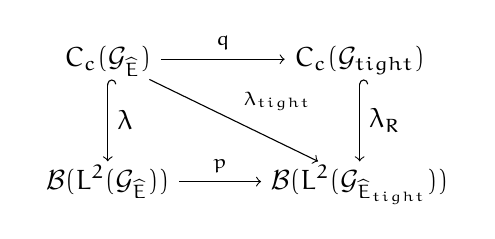
\begin{tikzpicture}
\matrix(m)[matrix of math nodes,row sep=3em, column sep=3em, text height=1.5ex, text depth = 0.25ex]
{C_{c}(\G_{\E})&C_{c}(\G_{tight})\\
\mathcal{B}(L^{2}(\G_{\E}))&\mathcal{B}(L^{2}(\G_{\E_{tight}}))\\};
\path[->,font=\scriptsize]
(m-1-1) edge node[auto] {$q$} (m-1-2)
(m-2-1) edge node[auto] {$p$} (m-2-2)
(m-1-1) edge node[auto] {$\lambda_{tight}$} (m-2-2);
\path[right hook->]
(m-1-1) edge node[auto] {$\lambda$} (m-2-1)
(m-1-2) edge node[auto] {$\lambda_{R}$} (m-2-2);

\end{tikzpicture}
\end{center}

where $\lambda_{R}$ is the left regular representation of $C_{c}(\G_{tight})$. It follows from the definition of $p$ that the bottom triangle commutes and the top triangle commutes as:
\begin{equation*}
\lambda_{x}(f) =\sum_{t \in \text{Max(S)}} f_{t}(x)\lambda_{x}(1_{tt^{*}}\delta_{t}) = \lambda_{x}(qf)
\end{equation*}
For each $x \in \E_{tight}$. Hence:
\begin{equation*}
\Vert qf \Vert_{r} = \sup_{x \in \E_{tight}} \lbrace \Vert \lambda_{x}(qf) \Vert \rbrace = \sup_{x \in \E_{tight}} \lbrace \Vert \lambda_{x}(f) \Vert \rbrace \leq \Vert \lambda(f) \Vert = \Vert f \Vert_{r}
\end{equation*}
and so $q$ is contractive (and therefore continuous).
 
Now to consider (2). It is enough to compute the result of products of elements of the form $f_{s}\delta_{s}$ for some $s \in \text{Max(S)}$. We then check the following two identities:


\begin{enumerate}[I]
\item $q(f_{s}\delta_{s} \Xst f_{t}\delta_{t}) = q(f_{s}\delta_{s})\Xst q(f_{t}\delta_{t})$
\item $(q(f_{s}\delta_{s}))^{*}=q((f_{s}\delta_{s})^{*})$
\end{enumerate}


To see (I) compute on a single element:
\begin{eqnarray*}
(f_{s}\delta_{s} \Xst f_{t}\delta_{t})([st,\phi])=f_{s}(\theta_{t}(\phi))f_{t}(\phi)
\end{eqnarray*}
Apply $q$:
\begin{eqnarray*}
q(f_{s}\delta_{s} \Xst f_{t}\delta_{t})([st,\phi])= (f_{s}\delta_{s} \Xst f_{t}\delta_{t})|_{\E_{tight}}([st,\phi]) =f_{s}(\theta_{t}(\phi))f_{t}(\phi)
\end{eqnarray*}
For all $[st,\phi] \in \G_{\E_{tight}}$. Then compute the right hand side: 
\begin{eqnarray*}
(q(f_{s}\delta_{s}) \Xst q(f_{t}\delta_{t}))([st,\phi])=f_{s}|_{\E_{tight}}(\theta_{t}(\phi))f_{t}|_{\E_{tight}}(\phi)
\end{eqnarray*}
Which matches for each $[st,\phi] \in \G_{\E_{tight}}$. 

To prove (II) we need to compute on a single element, where $(f_{s}\delta_{s})^{*}=\alpha_{s^{*}}(\overline{f_{s}})\delta_{s^{*}}$:

\begin{eqnarray*}
q((f_{s}\delta_{s})^{*})([s^{*},x])& = &\alpha_{s^{*}}(\overline{f_{s}})_{\E_{tight}}(x)\\
& = & \overline{f}(\theta_{s}(x)) \\ & = & \overline{f(\theta_{s}(x))} \\ & = & \overline{q(f)}(\theta_{s}(x)) \\ & = &  \alpha_{s^{*}}(\overline{q(f)})(x)
\end{eqnarray*}
Where the above holds for all $x \in \E_{tight}$ where the function $f_{s}$ is defined at $\theta_{s}(x)$ as required.

As $q$ is a continuous *-homomorphism, it extends to the completions.
\end{proof}

\subsection{Applying the machinery}\label{sect:S1-a}
We encode the norm estimations required for the proof of Theorem \ref{thm:PV1} in the following Lemma:
\begin{lemma}\label{lem:L3}
Let $S$ be F-inverse and let $K \subset \text{Max(S)}$ such that $K$ is finite and $T=\sum_{t \in K} a_{t}\lambda(1_{tt^{*}}\delta_{t})$ such that $a_{t}$ is the constant function that has value $a_{t}$ on $D_{tt^{*}}$. Then $\Vert T \Vert = \Vert qT \Vert$
\end{lemma}
\begin{proof}
It is immediate that $\Vert T \Vert \geq \Vert qT \Vert$ as $q$ is contractive. We arrive at the other inequality by applying Corollary \ref{cor:C1}.
\begin{eqnarray*}
\Vert T \Vert_{L^{2}(\mathcal{G}_{x})} = \Vert \sum_{t \in K} a_{t}\lambda_{x}(1_{tt^{*}}\delta_{t}) \Vert = \Vert \sum_{t \in K} a_{t}Q_{x}\lambda_{\infty}(1_{tt^{*}}\delta_{t})Q_{x}^{*} \Vert \\
= \Vert Q_{x}(\sum_{t \in K} a_{t}\lambda_{\infty}(1_{tt^{*}}\delta_{t}))Q_{x}^{*} \Vert = \Vert Q_{x}(qT)Q_{x}^{*} \Vert \leq \Vert qT \Vert.
\end{eqnarray*}
This holds for every $x \in E$ and so by  $\Vert T \Vert = \Vert \lambda(T) \Vert = \sup \lbrace \Vert \lambda_{x}(T) \Vert : x \in E \rbrace \leq \Vert qT \Vert$. This gives the desired equality.  
\end{proof}

\begin{theorem}\label{thm:PV1}
Let $S$ be an F-inverse monoid and let $\G_{\E}$ be its universal groupoid and let $A=C_{c}(\G_{U})$. Then we have the following (intrinsic) short exact sequence of $C^{*}$-algebras:
\begin{equation*}
0 \rightarrow \overline{A} \rightarrow C^{*}_{r}(\mathcal{G}) \rightarrow C^{*}_{r}(G) \rightarrow 0
\end{equation*}
\end{theorem}
\begin{proof}

We know that we have a surjective *-homomorphism $q$ from $C^{*}_{r}(\G)$ to $C^{*}_{r}(G)$, we just need to see that the kernel of this map is $\overline{A}$. The set $\overline{A}$ is contained in the kernel as elements in $A$ are sums of functions with value at $1_{E}=\infty \in \widehat{E}$ of zero and projection onto this value (i.e applying q) will send the entire element to $0 \in C^{*}_{r}(G)$. So it is enough to show that $A$ is dense in the kernel.

First consider finite sums. Let $f \in C_{c}(\mathcal{G})$. We need to show that if $qf=0$ then $ f \in A$.

$f$ has the form:
\begin{equation*}
f=\sum_{s \in S} f_{s}\delta_{s} \mbox{ } f_{s}\in C(D_{ss^{*}})
\end{equation*}
With only finitely many non-zero terms. This can be viewed concretely on $L^{2}(\mathcal{G})$ using
\begin{equation*}
\lambda(f)=\sum_{s \in S} f_{s}\lambda(1_{ss^{*}}\delta_{s})
\end{equation*}
As $S$ is F-inverse we can reduce this sum using the observation that for each $s \in S$ we can write the term $f_{s}\delta_{s}$ as $f_{s}\chi_{s}\delta_{t_{s}}$ where $t_{s}$ is the maximal element above $s$. So for each $t \in \text{Max(S)}$ we can define $f^{'}_{t}=\sum_{s \leq t}f(s)\chi_{s}$ and then
\begin{equation}\label{Eq1}
\lambda(f)=\sum_{t \in \text{Max(S)}} f^{'}_{t}\lambda(1_{tt^{*}}\delta_{t})
\end{equation}
(\ref{Eq1}) is in the kernel of $q$ if and only if each $f^{'}_{t}(\infty)=0$ for every $t \in \text{Max(S)}$ that is if and only if $\lambda(f) \in A$.

Now let $T$ be an element of $C^{*}_{r}(\G})$ such that $qT=0$. Then we need to show $T$ can be approximated by finite sums that lie in $A$. Let $T_{n}$ be finite sums in $C_{c}(\mathcal{G})$ with $T_{n} \rightarrow T$. Without loss of generality, these $T_{n}$ have the following form for some finite $K_{n} \subset \text{Max(S)}$:
\begin{equation*}
T_{n}=\sum_{t \in K_{n}} f^{n}_{t}\lambda(1_{tt^{*}}\delta_{t})
\end{equation*}
then $qT_{n} = \sum_{t \in K_{n}} f^{n}_{t}(\infty)\lambda_{\infty}(1_{tt*}\delta_{t})$. Define a pullback of $qT_{n}$:
\begin{equation}
S_{n} = \sum_{t \in K_{n}} a^{n}_{t}\lambda(1_{tt*}\delta_{t}) \in C_{c}(\mathcal{G})
\end{equation}
Where $a^{n}_{t}$ is the constant function on $D_{tt^{*}}$ with value $f_{t}^{n}(\infty)$. It is clear that $qS_{n}=qT_{n}$ and using Lemma \ref{lem:L3} we have that $\Vert S_{n} \Vert = \Vert qS_{n} \Vert = \Vert qT_{n} \Vert$ so $\Vert S_{n} \Vert \rightarrow 0$\\
\\
Let $U_{n}=(T_{n}-S_{n})$. Then $U_{n} \in A$ and $U_{n}=(T_{n}-S_{n}) \rightarrow (T-0)=T$, whence $A$ is dense in $ker(q)$.
\end{proof} 

\section{A similar sequence for 0-F-inverse monoids}\label{sect:S2}
In this section we consider a generalisation of Theorem \ref{thm:PV1} to strongly 0-F-inverse monoids with non-trivial K-exact universal group. We consider saturated subsets of the unit space as defined in Chapter 2. Clearly, subsets that are invariant under the action of $S$ are also saturated. The following Lemma outlines the connections between saturation and Morita enveloping actions.

\begin{lemma}\label{Lem:Cut}
Let $\G$ be an \etale locally compact Hausdorff groupoid with a (T,C,F)-cocycle $\rho$ to $\Gamma$. Then relation $\sim$ on $\G^{(0)} \times \Gamma$ preserves saturated subsets of $\G^{(0)}$
\end{lemma}
\begin{proof}
Let $U$ be a saturated subset of $\G^{(0)}$ and let $x \in U$, $y \in U^{c}$. Assume for a contradiction that $(x,g) \sim (y,h)$ in $\G^{(0)} \times \Gamma$. Then there exists a $\gamma$ $\in \G$ such that $s(\gamma)=x$, $r(\gamma)=y$ and $\rho(\gamma)=g^{-1}h$, but as $U$ is saturated no such $\gamma$ exists. 
\end{proof}

\begin{theorem}\label{thm:PV2}
Let $S$ be a strongly $0$-F-inverse monoid with universal group $G:=U(S)$. If $G$ is infinite and $K$-exact then the sequence:
\begin{equation*}
0 \rightarrow C^{*}_{r}(\G_{\U}) \rightarrow C^{*}_{r}(\G_{\E}) \rightarrow C^{*}_{r}(\G_{\E_{tight}}) \rightarrow 0
\end{equation*}
is exact at the level of K-theory.  
\end{theorem}
\begin{proof}
We begin by using either Theorem \ref{Thm:IT2-a} or \ref{Thm:IT2} to construct a transformation groupoid $Y_{\E}\rtimes G$ and a Morita equivalence between $\G_{\E}$ and $Y_{\E}\rtimes G$. We can repeat this process for both $\E_{tight}$ and $U:=\E_{tight}^{c}$, and by Lemma \ref{Lem:Cut} and the fact that $\E_{tight}$ is closed in $\E$ we can conclude that we have a natural sequence of commutative $C^{*}$-algebras:
\begin{equation*}
0 \rightarrow C_{0}(Y_{U}) \rightarrow C_{0}(Y_{\E}) \rightarrow C_{0}(Y_{\E_{tight}}) \rightarrow 0
\end{equation*}
each of which is a $G$-algebra. We now act by the reduced cross product, which produces a sequence of $C^{*}$-algebras:
\begin{equation*}
0 \rightarrow C_{0}(Y_{U})\rtimes_{r}G \rightarrow C_{0}(Y_{\E})\rtimes_{r}G \rightarrow C_{0}(Y_{\E_{tight}})\rtimes_{r}G \rightarrow 0.
\end{equation*}
This may not be exact in the middle term. However, it is exact at the level of K-theory, so consider the K-theory long exact sequence:
\begin{equation*}
\xymatrix@=1em{...\ar[r] & K_{0}(C_{0}(Y_{U})\rtimes_{r} G) \ar[r]& K_{0}(C_{0}(Y_{\E})\rtimes_{r} G) \ar[r]& K_{0}(C_{0}(Y_{\E_{tight}})\rtimes_{r} G)\ar[r] & ...\\
...\ar[r] & K_{0}(C^{*}_{r}(\G_{\U})) \ar[r]\ar[u]^{\ucong}& K_{0}(C^{*}_{r}(\G_{\E})) \ar[r]\ar[u]^{\ucong}& K_{0}(C^{*}_{r}(\G_{\E_{tight}})) \ar[r]\ar[u]^{\ucong}& ...}
\end{equation*}
where the isomorphisms are induced by the Morita equivalences given by Theorems \ref{Thm:IT2-a} and \ref{Thm:IT2}. This concludes the proof.
\end{proof}


\section{Translation Structures to Inverse Monoids}
In this section we outline the definition of a partial translation structure and describe some of the results concerning them from the literature. Focusing on a special case, which we call \textit{grouplike partial translation structures}, we connect uniform embeddability into groups for metric spaces to translation structures.  We then outline an inverse monoid approach to understanding the translation algebra that can be naturally associated to a partial translation structure.

The concept of a partial translation structure was first introduced in \cite{MR2363428}. By associating to a metric space this additional information, namely a collection of partial bijections that form entourages in the metric coarse structure, it is possible to use the local symmetries of the space to control the metric. 


\begin{definition}\label{PT2}
A partial translation structure on $X$ is a collection $\mathcal{T}$ of partial translations of $X$ such that for all $R>0$ there exists a finite subset $\mathcal{T}_{R}$ of disjoint partial translations in $\mathcal{T}$ and a collection $\Sigma_{R}$ of partial cotranslations of $\mathcal{T}_{R}$ satisfying the following axioms:
\begin{enumerate}
\item The union of the partial translations  $t \in \mathcal{T}_{R}$ contains the R-neighbourhood of the diagonal.
\item There exists $k$ such that for each $x,x^{'} \in X$ there are at most $k$ elements $\sigma \in \Sigma_{R}$ such that $\sigma x=x^{'}$.
\item For each $t \in \mathcal{T}_{R}$ and for all $(x,y),(x^{'},y^{'}) \in t$ there exists $\sigma \in \Sigma_{R}$ such that $\sigma x=x^{'}$ and $\sigma y=y^{'}$.
\end{enumerate}
\end{definition}

\begin{definition}(Freeness, Global control)
A partial translation structure on X is said to be \textit{free} if in Definition \ref{PT2} ii) $k=1$; i.e there is a unique cotranslation such that for each pair $(x,y)\in X \times X$ we have $\sigma x = y$.\\
A partial translation structure on X is said to be \textit{globally controlled} if the partial cotranslation orbits are partial translations. 
\end{definition}

The following is Theorem 19 from \cite{MR2363428}.

\begin{lemma}\label{lem:L10}
Let $G$ be a group equipped with a proper left invariant metric and let $X \subseteq G$ equipped with the induced metric. Then the restriction of the action of $G$ on itself by right multiplication to $X$ is a partial translation structure that is free and globally controlled.
\end{lemma}

The intuition for the Definition \ref{PT2} is a metric version of a group action for spaces, with freeness and global control giving conditions that are similar to a free and transitive action of group. 

\begin{definition}\label{def:ZD1}
Let $\mathcal{T}$ be a partial translation structure. Then we say $\mathcal{T}$ has \textit{zero divisors} if there exists a product of disjoint translations $t_{1},t_{2},...,t_{n} \in \mathcal{T}$ such that $t_{1}t_{2}t_{3}...t_{n}$ is empty (i.e has empty domain). We say $\mathcal{T}$ has no zero divisors if no such product is empty.
\end{definition}
We specialize our definition slightly in light of the following proposition, the proof of which can be found in \cite[Proposition 8.1]{rosiesthesis}

\begin{proposition}\label{prop:TFAE} Let $G$ be a countable discrete group and let $X \subseteq G$
The following are equivalent:
\begin{enumerate}
\item $X^{c}$ is not coarsely dense in $G$.
\item For every $R>0$ there exists $g \in G$ such that $B_{R}(g) \subseteq X$.
\item The monoid generated by $\mathcal{T}_{G}|_{X}$ has no zero element.
\end{enumerate}
\end{proposition}
The definition provided below is stronger than the definition provided in \cite{MR2363428}, however this better emulates the situation that arises when you consider a space that is uniformly embedded into a group.

\begin{definition}\label{Def:PTS}
Let $X$ be a countable discrete metric space. A collection of partial bijections $\mathcal{T}$ is a called a \textit{grouplike partial translation structure} for $X$ if:
\begin{enumerate}
\item $\mathcal{T}$ partitions $X\times X$.
\item $\forall t_{i}, t_{j} \in \mathcal{T}$ $\exists t_{k} \in \mathcal{T}$ we have $t_{i}t_{j} \subseteq t_{k}$ (i.e $\mathcal{T}$ is subclosed).
\item $\forall t \in \mathcal{T}$ we have $t^{*} \in \mathcal{T}$.
\item $\mathcal{T}$ has a global identity, denote this $t_{0}$.
\end{definition}

As a consequence of the Wagner-Preston Theorem \cite{MR1455373} partial bijections move us toward inverse semigroup theory.
\begin{proposition}\label{prop:P6}
Let $X$ be a metric space equipped with a group-like partial translation structure $\mathcal{T}$. Then $\mathcal{T}$ generates an inverse submonoid of $I_{b}(X)$
\end{proposition}
\begin{proof}
The axioms for a grouplike structure tell us that for every translation we have the adjoint translation - that acts an inverse. As $\mathcal{T}$ partitions $X \times X$ $t^{*}$ is unique for every $t \in \mathcal{T}$. These elements are partial bijections on $X$, and so are elements of $I_{b}(X)$ and we can consider the subsemigroup they generate. As each element of this subsemigroup has a unique inverse we get that it must be an inverse subsemigroup. The presence of the global identity map in $\mathcal{T}$ will give a global identity in the subsemigroup it generates. Hence the subsemigroup is a submonoid, as required.
\end{proof}

We can characterise the monoids generated by partial translation structures:

\begin{lemma}\label{Lem:PTS}
The inverse monoid $S$ generated by a partial translation structure $\mathcal{T}$ is 0-F-inverse, with maximal element set $\lbrace t_{i} : t_{i} \in \mathcal{T} \rbrace$. 
\end{lemma}
\begin{proof}
First we prove maximality of the translations. We prove that for any $s\in S \setminus \lbrace 0 \rbrace$ there exists a unique $t \in \mathcal{T}$ such that $s \leq t$. Property (2) from the Definition \ref{Def:PTS} implies that $\mathcal{T}$ generates the partial order on $S$. As $\mathcal{T}$ partitions $X \times X$ we have that for any pair $t_{i},t_{j}\in \mathcal{T}$ $et_{i}=et_{j} \Leftrightarrow t_{i}=t_{j}$. 

Now we prove that $S$ is $0$-E-unitary. Let $e\in E(S)\setminus \lbrace 0 \rbrace$ and $s\in S\setminus \lbrace 0 \rbrace$. Without loss of generality we can treat $s$ as maximal in what follows. Assume that $e \leq s$. This gives us two equations: $es=e \leq s$. As the natural order is preserved by taking inverses we see that $s^{*}e \leq s^{*}$. These imply that $s=s^{*}$. This tells us that $s^{2}$ is idempotent, but we want $s$ idempotent. To show this we will aim for $s^{2}=s^{3}$. Observe that $es=es^{2}\leq s^{2} \leq s$. This implies $s^{2}=fs$ for some $f\in E(S)$. $s^{3}=s^{2}s=(fs)s=f^{2}s=fs=s^{2}$. As $s=s^{3}$ we get $s \in E(S)$ as required.
\end{proof}

\subsection{An Embeddability Theorem for Metric Spaces with Grouplike Partial Translation Structures.}

The precise nature of the relationship between partial translation structures in the sense of Definition \ref{Def:PTS} and uniform embeddings is understood. It follows from Theorem 19 of \cite{MR2363428} that given any space that admits a uniform embedding into a group, we can equip it with a translation structure given by the Definition \ref{Def:PTS}. The inverse monoid generated by this translation structure is also understood from Lemma \ref{Lem:PTS}.

In this section we provide a partial converse to Theorem 19 of \cite{MR2363428}:

\begin{theorem}\label{thm:T2}
Let $X$ be a countable discrete metric space equipped with a grouplike partial translation structure $\mathcal{T}$, where $\mathcal{T}$ has no zero divisors. Then there exists a countable discrete group $G$ and an embedding $X \hookrightarrow G$ such that the translation structure provided by $G$ restricted to $X$ denoted $\mathcal{T}_{G}|_{X}$ is equal to $\mathcal{T}$.
\end{theorem}

\begin{proof}
Consider the inverse monoid $S = \langle \mathcal{T} \rangle$. $\mathcal{T}$ has no zero divisors implies that $S/\sigma$ is a non-trivial group. Denote that group by $G$. The aim now is to embed $X$ into $G$. The maximal elements in $\mathcal{T}$ generate this group, and $\sigma$ induces an inverse semigroup homomorphism from $S$ into $G$, which is a bijection between the maximal elements and $G$. Denote by $T_{x_{0}}$ the following:
\begin{equation}
T_{x_{0}} := \lbrace t \in \mathcal{T} : tx=x_{0} \rbrace
\end{equation}
where $x_{0}$ is a basepoint in $X$. Observe that because $\mathcal{T}$ partitions $X \times X$ we can construct a bijection between $X$ and $T_{x_{0}}$. Restricting to the image of $T_{x_{0}}$ under $\sigma$ we get a subspace of the group that is in bijection with $X$, i.e we can view $X$ as a subset of the group $G$. To finish the proof, we need the translation structure $\mathcal{T}$ to come from the group. We can construct this as follows. Take a translation $t_{j} \in \mathcal{T}$. For every $x \in Dom(t_{j})$ there exists a unique $t_{x} \in T_{x_{0}}$ such that $t_{x}x=x_{0}$. For each $x \in Dom(t_{j})$ there exists a unique $y \in X$ such that $t_{j}x=y$ Taking adjoints: $t_{j}^{*}y=x$. This gives a map: $t_{x}t_{j}^{*}y=x_{0}$ and $y$ corresponds to some element in $T_{x_{0}}$, denote this $t_{y}$. This gives the following situation:
\begin{equation}
t_{x}t_{j}^{*} \subseteq t_{y}.
\end{equation} 
Under $\sigma$ we have:
\begin{equation}
g_{x}g_{j}^{-1}=g_{y}
\end{equation}
This action on the right by inverses agrees with the typical translation structure of a group restricted to $X$, as we can define:
\begin{equation}
t_{g_{j}}:g_{x} \mapsto g_{y}, \mbox{ using $\sigma$; } x \mapsto y
\end{equation}
And this construction holds for all $x\in Dom(t_{j})$. This tells us that $Dom(t_{j}) \subseteq Dom(t_{g_{j}})$. All that remains is to show the reverse inclusion. Let $h \in Dom(t_{g_{j}})$ Then $h \in X \cap Xg_{j}$ so $h=h^{'}g_{j}$ and:
\begin{equation}
t_{g_{j}}:h \mapsto h^{'}
\end{equation}
Pulling $h$ and $h^{'}$ back into $X$ using the original bijection, we get a pair $(x,y) \in X \times X$. As $\mathcal{T}$ partitions $X\times X$ we have a unique $t_{p} \in \mathcal{T}$ such that $t_{p}x=y$. Via $\sigma$ we get the following situation:
\begin{equation}
h=h^{'}g_{p}=h^{'}g_{j} \Leftrightarrow g_{p}=g_{j}
\end{equation}
And pulling back this gives us $t_{p}=t_{j}$. So for every point $x\in Dom(t_{g_{j}})$ we have that $x \in Dom(t_{j})$.

Hence for each map in $\mathcal{T}$ we have a corresponding map in $\mathcal{T}_{G}|_{X}$ which is defined in the same places and is equal where it is defined. This implies $\mathcal{T}=\mathcal{T}_{G}|_{X}$ s required.
\end{proof}

The following is a direct corollary of Theorem \ref{thm:T2} and Proposition \ref{prop:TFAE}:

\begin{corollary}
The compliment of $\sigma (T_{x_{0}})$ is not coarsely dense in $G$.\qed
\end{corollary}


In summary, Theorem \ref{thm:T2} provides us a wealth of examples of F-inverse monoids with the added information of a concrete representation on an interesting metric space. It turns out that this provides a simplification to Theorem \ref{thm:PV1} when dealing with such representations.

\subsection{Translation Algebras}
Let $X$ be a uniformly discrete bounded geometry metric space.

\begin{definition}
The translation algebra associated with a partial translation structure $\mathcal{T}$ on $X$, denoted by $C^{*}\mathcal{T}$, is the completion as a *-subalgebra of $\mathcal{T}$ viewed as bounded operators on $\ell^{2}(X)$
\end{definition}

The aim of this section is to give a description of the partial translation algebra associated to a grouplike partial translation structure $\mathcal{T}$ with no zero divisors as the $C^{*}$-algebra of a groupoid, where the groupoid is related to the inverse monoid generated by the partial translations. We then recast Theorem 8.3 of Brodzki, Niblo, Putwain and Wright \cite{rosiesthesis} outlining a short exact sequence of $C^{*}$-algebras arising from such translation structures and compute some examples in certain cases.

Given the information of Lemma \ref{Lem:PTS} we have a inverse monoid that we can associate to a grouplike translation structure. This has a natural $C^{*}$-algebra, as outlined in Chapter 2. However, we have not used the geometric representation of this inverse monoid on $I(X)$, which determines a representation on $\ell^{2}(X)$ in the standard way. This representation will be the focus of this section. The following is Proposition 10.6 \cite{MR2419901}

\begin{proposition}\label{prop:P7} 
Let $\mu$ be a representation of $S$ on a Hilbert Space $H$. Then there exists a unique *-representation $\pi_{\mu}$ of $C_{0}(\E)$ on $H$ such that $\pi_{\mu}(1_{e})=\mu(e)$ for every $e \in E$ In addition $(\pi_{\mu} \times \mu)$ is a covariant representation for $\G_{\E}$. 
\end{proposition}

The proof of the above result relies on the spectrum of the commutative $C^{*}$-subalgebra $A=C^{*}_{\pi_{\mu}}(E)$ of $C^{*}_{\pi_{\mu}}(S)$. We denote the spectrum by $\X$. The key aspect of the proof of Proposition \ref{prop:P7} is the natural injective continuous map $j$ defined by: 
\begin{equation*}
j: \psi \in \X \mapsto \phi = \psi \circ \sigma \in \E
\end{equation*}

So given $X$ equipped with a grouplike partial translation structure with no zero divisors $\mathcal{T}$, we get an inverse monoid $S=\langle \mathcal{T} \rangle$ and a representation $\mu: S \hookrightarrow I_{b}(X)$ from Proposition \ref{prop:P6}. So applying Proposition \ref{prop:P7} we arrive at a representation $\pi_{\mu}$ of $C(\E)$ on $\ell^{2}(X)$. 

\begin{proposition}\label{prop:P9}
Let $S$ be a 0-F-inverse monoid and let $\mu: S \hookrightarrow I_{b}(X)$ be a geometric representation. Then the following hold for $\X$: \begin{enumerate}
\item $\X \hookrightarrow \E$ is a topological embedding
\item $\beta X \twoheadrightarrow \X$ is a quotient map.
\end{itemize}
Moreover the topologies are all compatable with the topology endowed as the spectrum of $A=C^{*}_{\pi_{\mu}}(E)$.
\end{proposition}
\begin{proof}
We give a concrete proof when $S$ has no 0: First we show (1) using the map $j$ defined above. $j(\X)$ is compact as j is continous and closed because $\E$ is Hausdorff.

For (2) we observe that the quotient map is given by the equivalence relation 
\begin{equation*}
\phi \sim \phi^{'} \leftrightarrow \phi \cap E(S) = \phi^{'} \cap E(S)
\end{equation*}
This map is surjective as given any $\psi \in \X$ we can view this as a filter on $X$ be considering the set:
\begin{equation*}
F_{\psi} = \lbrace e \in E(S) | \psi(\sigma(e))=1 \rbrace
\end{equation*}
We can complete this to an ultrafilter in $\beta X$ in many ways using Zorn's Lemma, however it is enough to show we can do it such that $F_{\psi ,UF}\cap E(S) = \psi$. So it is enough to pick subsets according to the following rules. Let $M,M^{c} \in \lbrace 0,1 \rbrace^{X}$ and
\begin{itemize}
\item If $M \in E(S)$ then add $M^{c}$ to $F_{\psi}$
\item If $M \not\in E(S)$ then add $M$ to $F_{\psi}$
\item If $M,M^{c} \not \in E(S)$ add either to $F_{\psi}$
\end{itemize}
With the case in which both $M$ and $M^{c}$ are contained in $E(S)$ is impossible as $E(S)$ has no zero element.

Now $F_{\psi}$ has the correct property and is an ultrafilter of $\beta X$ that maps onto $\psi$. Observe that the image of $\beta X$ is again compact, and thus closed, hence the map is a quotient.

In the case that $S$ has a zero element, we appeal to universal properties and another result of Exel \cite{MR2419901}. By Proposition 10.10 \cite{MR2419901} the space $\widehat{X}$ is closed and invariant.

Recall each $t \in \mathcal{T}$ is an element of $I_{b}(X)$ implies that the algebra $C^{*}_{\pi}(S)$ is a subalgebra of the uniform Roe algebra $C^{*}_{u}X$. We now remark that the representation $\pi_{X}$, when restricted to $C^{*}E$ assigns each idempotent a projection in $C^{*}_{u}X$, that is $C^{*}_{\pi_{\mu}}(E)=\pi_{}(C^{*}E) \subset \ell^{\infty}(X)$. Taking the spectra associated to this inclusion then gives us a map:
\begin{equation*}
r_{\beta X}: \beta X \twoheadrightarrow \widehat{X}
\end{equation*}
which is continuous. In particular as both $\beta X$ and $\widehat{X}$ are compact Hausdorff spaces, this map is closed (and open) and hence a quotient.
\end{proof}

\begin{corollary}\label{cor:C3}
Let $\psi_{x} = \lbrace x \rbrace^{\uparrow} \cap E(S)$. Then the set $\lbrace \psi_{x} | x \in X \rbrace$ is dense in $\X$.
\end{corollary}

In the most general situation the subspace $X$ may be stabilized under the right or left action of the group; we denote the left stablizer $LStab_{G}(X)$ by $H$. 

\begin{proposition}\label{prop:P9a}
$x_{1}x_{2}^{-1} \in H \Leftrightarrow \forall t \in \mathcal{T} (x_{1} \in Dom(t) \Leftrightarrow x_{2} \in Dom(t))$
\end{proposition}
\begin{proof}
($\Rightarrow$) $x_{1}x_{2}^{-1} \in H$ is equivalent to $x_{1}, x_{2} \in Hx$ for some $x \in X$. This implies that $(x_{1} \in Dom(t) \Leftrightarrow x_{2} \in Dom(t))$ as the elements of $H$ are contranslations of $X$. 

In fact we can say that the elements of $H$ are precisely the cotranslations that are bijections of $X$. This is key in proving the converse:

($\Leftarrow$) Consider $h=x_{1}x_{2}^{-1}$. We want to see that for all $x \in X$ $hx \in X$. Observe that by the first property of translation structures there exists a unique translation $t$ such that $t(x_{2})=x$ Then $hx=ht(x_{2})=t(hx_{2})=t(x_{1}) \in X$ and this chain of equalities holds precisely when $(x_{1} \in Dom(t) \Leftrightarrow x_{2} \in Dom(t))$

\end{proof}

\begin{corollary}\label{cor:C5}
$B$ is in bijection with $H \backslash X$
\end{corollary}
\begin{proof}
The righthand side of Proposition \ref{prop:P9a} is equivalent to the condition that $\psi_{x_{1}}=\psi_{x_{2}} \in B$.
\end{proof}

It is immediate (using \cite[Prop 10.10]{MR2419901}) that the set $\X$ is invariant under the action of $S$. To compute the groupoid and groupoid $C^{*}$-algebras associated to $\X$ we would like to know a little more about the Hilbert spaces associated to the fibers and general connectness of the set $B:=\lbrace \psi_{x} | x \in X \rbrace$ (which using Corollary \ref{cor:C3} is dense in $\X$).

\begin{proposition}\label{prop:P10}
Let $t \in \mathcal{T}$. Then $\theta_{t}(\psi_{x})=\psi_{t(x)}$ for all $x \in Dom(t)$.
\end{proposition}
\begin{proof}
First some observations:
\begin{enumerate}
\item $\theta_{t}(\psi_{x})$ is defined as $\theta_{t}(\psi_{x}) \in D_{tt^{*}} \Leftrightarrow \psi_{x} \in D_{t^{*}t} \Leftrightarrow t^{*}t \in \psi_{x} \Leftrightarrow x \in t^{*}t = Dom(t)$.
\item $(\theta_{t}(\psi_{x}))(tet^{*})=\psi_{x}(t^{*}(tet^{*})t)=\psi_{x}(e)$. Hence $e \in \psi_{x} \Leftrightarrow tet^{*}  \in \theta_{t}(\psi_{x})$.
\item $\psi_{x}=\psi_{y} \Leftrightarrow \psi_{t(x)}=\psi_{t(y)}$, in fact more is true as: $\psi_{t(x)}=\psi_{t^{'}(y)} \Leftrightarrow Dom(t^{'})=Dom(t)$.
\end{enumerate}
We prove inclusions. First $\theta_{t}(\psi_{x}) \subset \psi_{t(x)}$. Without loss of generality, we can take $tet^{*}$ to be the general form of an element of $\theta_{t}(\psi_{x})$ and then: $tet^{*} \in \psi_{t(x)} \Leftrightarrow t(x) \in tet^{*} \Leftrightarrow tet^{*}(t(x))=t(x)$, which is the case if and only if $e \in \psi_{x}$.

To see the reverse inclusion let $f \in \psi_{t(x)}$. Then $f \in \theta_{t}(\psi_{x}) \Leftrightarrow t^{*}ft \in \psi_{x} \Leftrightarrow t(x) \in f \Leftrightarrow f \in \psi_{t(x)}$. 

To conclude; (3) controls the behavior of the action when the stabilizer is non-trivial, the first part shows the action behaves with respect to the quotient and the second part shows that given any pair $(x^{'},y^{'})\in X \times X$ such that $x^{'}\in Hx, y^{'}\in Ht(x)$ the unique translation $t_{x^{'}y^{'}} \in \mathcal{T}$ that sends $x^{'}$ to $y^{'}$ defines an arrow between $\psi_{x}$ and $\psi_{t(x)}$. 
\end{proof}

\begin{proposition}\label{cor:C4}
$B$ is invariant and $\G_{B}$ is connected. Moreover if $H$ is trivial, then $B$ is invariant and $\G_{B}$ is uniquely connected.
\end{proposition}
\begin{proof}
$B$ is invariant as a consequence of Proposition \ref{prop:P10}, and connected by the first property of grouplike partial translation structures - $\mathcal{T}$ partitions $X \times X$. This tells us that when we pass to the quotient $H \backslash X$ we get a collection of arrows between each pair of points that are indexed by $H$. 

In the situation that $H$ is trivial we get a unique arrow between any two points in $B$ and $B$ is in bijection with $X$, hence the groupoid $\G_{B}$ is precisely the pair groupoid $X \times X$, with the norm coming from the stalks, each of which have the form of $\ell^{2}(X)$ by the uniquely connected property of $B$.
\end{proof}

\begin{remark}
In the situation that $H$ is non-trivial, we have a unit space for $\G_{B}$ that is $B\times B$, with arrows between each pair indexed by $H$. The Hilbert space associated to each fibre $L^{2}(\G_{\X})|\psi_{x}$ is exactly the Hilbert space with basis indexed by the \textit{arrows} $[t_{h},\psi_{x}]$ - the set of arrows based at $\psi_{x}$ is in bijection with $X$, construct a map using the first property of translation structures.

For each point $hx \in Hx$ there exists a unique translation $t_{y,h}$ to each other point $y \in X$. We then define the map $[t_{y,h}, \psi_{x}] \mapsto t_{y,h}(hx)=y$.

This provides a unitary isomorphism between these spaces, denote this map at the level of Hilbert spaces by $U_{x}$ for each $x \in H \backslash X$.
\end{remark}

\begin{proposition}\label{prop:P11}
$\Vert \lambda(1_{tt^{*}}\delta_{t}) \Vert = \Vert \mu(t) \Vert_{\ell^{2}(X)}$ for all $t \in \mathcal{T}$. 
\end{propositon}
\begin{proof}
The proof of this fact follows from a computation on the basis of $\ell^{2}(X)$ using the unitary isomorphism $U_{x}$. We compute $U_{x}\lambda_{\psi_{x}}(1_{tt^{*}}\delta_{t})U_{x}^{-1}$ evaluated on a basis element $\delta_{y} \in \ell^{2}(X)$.
\begin{enumerate}
\item $U_{x}^{-1}(\delta_{y})=\delta_{[t_{y,h},\psi_{x}]}$
\item $\lambda_{\psi_{x}}(1_{tt^{*}}\delta_{t})(\delta_{[t_{y,h},\psi_{x}]})(\delta_{[s,\psi_{x}]})=\sum_{\substack{[n,\psi_{z}][u,\psi_{x}]\\=[s,\psi_{x}]}} 1_{tt^{*}}([n, \psi_{z}]\delta_{[t_{y,h},\psi_{x}]}([u,\psi_{x}])=\delta_{[t_{y,h},\psi_{x}]}$

Hence $\lambda_{\psi_{x}}(1_{tt^{*}}\delta_{t})$ moves the basis element $\delta_{[t_{y,h},\psi_{x}]}$ to the basis element $\delta_{[s,\psi_{x}]}$, where $s$ is the unique translation above $tt_{y,h}$ in $\mathcal{T}$.
\item $U_{x}(\delta_{[tt_{y,h},\psi_{x}]})=\delta_{t(t_{y,h}(hx))}=\delta_{t(y)}=\mu(t)(\delta_{y})$.
\end{enumerate}
This holds for all $y$ in the domain of $t$, as the multiplication in the groupoid is defined for only that situation.

As we have this equality for each $\psi_{x} \in B$; we get that $\Vert \lambda(1_{tt^{*}}\delta_{t}) \Vert_{r} = \sup \lbrace \Vert \lambda_{\psi_{x}}(1_{tt^{*}}\delta_{t}) \Vert : \psi_{x} \in B \rbrace = \Vert \mu(t) \Vert_{\ell^{2}(X)}$.
\end{proof}
\end{proposition}

This extends to finite sums:

\begin{lemma}\label{lem:L7}
Let $K \subset \X$ be a finite subset and let $a_{t}$ be the constant function valued $a_{t}$ on $D_{tt^{*}}$. Then \Vert \sum_{t \in K} a_{t}\delta_{t} \Vert_{r} = \Vert \sum_{t \in K} a_{t} \mu(t) \Vert_{\ell^{2}(X)}  
\end{lemma}
\begin{proof}

First we show that $\sum_{t \in K} a_{t}\delta_{t}$ represents as $\sum_{t \in K} a_{t} \mu(t)$ on the basis of $\ell^{2}(X)$. We proceed as in proposition \ref{prop:P10}. 

First compute $U_{x}^{-1}(\delta_{y})$:
\begin{equation*}
U_{x}^{-1}(\delta_{y})=\delta_{[t_{y,h},\psi_{x}]}
\end{equation*}
Then compute: 
\begin{eqnarray*}
(\sum_{t \in K}\lambda_{\psi_{x}}(a_{t}\delta_{t}))(\delta_{[t_{y,h},\psi_{x}]})& = &\sum_{\left\lbrace t\in K:\substack{[t,\psi_{y}][t_{y,h},\psi_{x}]\\=[tt_{y,h},\psi_{x}] }\right\rbrace} a_{t}([t, \psi_{y}])\delta_{[t_{y,h},\psi_{x}]}([t_{y,h},\psi_{x}])\\
& = &\sum_{\lbrace t \in K, y \in Dom(t)\rbrace }a_{t}([t,t_{y,h}(\psi_{x})])\delta_{[tt_{y,h}, \psi_{x}]}\\ & = &\sum_{t \in K,y \in Dom(t)}a_{t}\delta_{[tt_{y,h}, \psi_{x}]}
\end{eqnarray*}
Lastly move back to $\ell^{2}(X)$ via $U_{x}$:
\begin{eqnarray*}
U_{x}(\sum_{t \in K,y \in Dom(t)}a_{t}\delta_{[tt_{y,h}, \psi_{x}]}) & = &\sum_{t \in K, y \in Dom(t)}a_{t}\delta_{t(y)}\\ & = &(\sum_{t \in K}a_{t}\mu(t))(\delta_{y})
\end{eqnarray*}

\end{enumerate}

So both finite sums transform the basis in the same way. This equality holds for each $\psi_{x}$ in $B$, so we can conclude that $\Vert \sum_{t \in K} a_{t}\delta_{t} \Vert_{r} = \sup \lbrace \Vert \lambda_{\psi_{x}}(\sum_{t \in K} a_{t}\delta_{t} ) \Vert : \psi_{x} \in B \rbrace = \Vert \sum_{t \in K} a_{t} \mu(t) \Vert_{\ell^{2}(X)}$.
\end{proof}

This lets us define a map: 
\begin{equation*}
\mathcal{Q}: \lambda(1_{tt^{*}}\delta_{t}) \mapsto \mu(t)
\end{equation*}

Now we can state and prove the main result of this section:
\begin{theorem}\label{thm:T5}
Let $X \subset G$, giving us a translation structure $\mathcal{T}_{G}|_{X}$ with no zero divisors and a representation $\mu: S = \langle \mathcal{T}_{G}|_{X} \rangle$. Then we have an isomorphism C^{*}_{r}(\G_{\X}) \cong C^{*}_{\mu}(S) = C^{*}\mathcal{T}. 
\end{theorem}

\begin{proof}
The map $\mathcal{Q}$ is surjective onto $\mathbb{C}S$ (mapping to the generators of $S$), so it remains to see that it passes to the completion and is injective. 
To show this, we appeal to Lemma \ref{lem:L7} to show that the norms match under the map $\mathcal{Q}$ up to finite sums - making the map on the incomplete algebras uniformly continous. Ideally, we would now complete - however we need to be careful as the incomplete *-algebra $M$ generated by finite sums of $1_{e}\delta_{t}$ may not be dense (and is the source of the map $\mathcal{Q}$).

However we observe that by the Stone-Weierstrass Theorem every element in $C(\X)$ can be approximated by elements of the form $1_{e}$, i.e for all $f_{t} \in C(\X)$:
\begin{equation*}
f_{t} = \lim_{n} (\sum_{e \in E} a^{n}_{e}1_{e})
\end{equation*}
So for a particular element  $f=\sum_{t \in K}f_{t}\delta_{t} \in C_{c}(\G_{\X})$ we can approximate each $f_{t}$ in turn by limits of $\sum_{e \in E} a_{e}1_{e}$ giving us an approximation by finite sums of elements in $M$. Hence $\overline{M} = C^{*}_{r}(\G_{\X})$, allowing $\mathcal{Q}$ to pass to completions (by uniform continuity).

After passing to the completion, the map is isometric; hence injective. This gives us the first isomorphism. To see the equality, observe that by definition the translation algebra is the algebra generated in $\mathcal{B}(\ell^{2}(X))$ by the set of operators $\lbrace \mu(t) | t \in \mathcal{T} \rbrace$. This is precisely $C^{*}_{\mu}(S)$.
\end{proof}

\subsection{A Short Exact Sequence of Translation Algebras}

In this situation we still have access to all the tools available in the general inverse monoid case, as well as all the geometric properties arising from the representation $\mu$.

\begin{theorem}\label{thm:T4}
Let $X \subset G$, $\mathcal{T}=\mathcal{T}_{G}|_{X}$ be a grouplike partial translation structure on $X$ with no zero divisors and $S=\langle \mathcal{T} \rangle \hookrightarrow_{\mu} I(X)$ be the associated F-inverse monoid. Then we have the following short exact sequence of $C^{*}$-algebras:
\begin{equation}\label{eqn1}
0 \rightarrow C^{*}_{r}(\G_{U}|_{\X}) \rightarrow C^{*}_{r}(\G_{\X}) \rightarrow C^{*}_{r}(G) \rightarrow 0
\end{equation}
Where the middle term is the translation algebra associated to $X$ arising from $\mathcal{T}$
\end{theorem}
\begin{proof}
The proof follows the same lines as the proof of Theorem \ref{thm:PV1}.
\begin{enumerate}
\item The map defined on finite sums still has the desired properties, i.e a finite sum is in the kernel if and only if all its components are 0.
\item We still have the same pullbacks of constant functions to the entire space; This enables the same construction of approximating elements; who each have the same norm control property provided by Corollary \ref{cor:C1}.
\item We can then conclude that the kernel is the desired algebra with a density argument.
\end{enumerate}
\end{proof}

%\setstretch{1.6}
\chapter{Counterexamples to Baum-Connes and Large Girth Expanders.}
In this chapter we develop the basic concepts of coarse geometry for metric spaces and outline some coarse properties that can be associated to a metric space. We then outline certain analytic group and groupoid properties and connect these to their coarse counterparts. Secondly, we introduce the coarse Baum-Connes conjecture for proper metric spaces and outline machinery to construct counterexamples to this conjecture by converting the coarse assembly map into a groupoid assembly map.

We then present a unifying approach to all known counterexamples to this conjecture by developing the groupoid centric viewpoint of \cite{MR1911663} further, introducing a new conjecture known as the \textit{boundary coarse Baum-Connes conjecture}. First however we outline the construction of the algebras involved in defining the coarse assembly map $\mu$, then make some connections to groupoid equivariant KK-theory. These ideas then allow us to formulate the boundary coarse Baum-Connes conjecture and apply homological algebra techniques to connect it to the coarse Baum-Connes conjecture.

As an example of the flexibility of this new conjecture we verify it for certain large classes of expander graph, generalising work of Willett and Yu \cite{explg1}.

\section{Coarse geometry, Groupoids and Assembly.}
In this section we outline the coarse geometry and group theoretic properties that are going to be considered throughout this chapter. The overall scheme of this section is first to consider some general coarse ideas associated to metric spaces and then move onto discussions of certain analytic properties held by discrete groups. We will develop these coarse ideas further by introducing abstract coarse structures and their relationship to metric spaces.

\subsection{Coarse geometry.}
The notions of coarse geometry are similar in spirit to those of topology, however the focus is on the large as opposed to the small. Recall that a function $f$ between topological spaces $X$ and $Y$ is continuous if the preimage of every open set in $Y$ is open in $X$. Suppose additionally that $X$ and $Y$ are metric spaces equipped with the metric topology. The key idea in coarse geometry is somehow to supplant this notion of continuous by replacing the occurrences of open in the definition with \textit{bounded}. We call such maps \textit{metrically proper}. If additionally suppose that the map $f$ sends sets of diameter $R$ to sets of diameter at most $S$ for some $S>0$. Then we call such a map \textit{bornologous}. Combining these two, we arrive at a definition:

\begin{definition}
Let $f:X \rightarrow Y$ be a map of metric spaces. $f$ is \textit{coarse} if it is both metrically proper and bornologous.
\end{definition}

A coarse map, intuitively, preserves the structure of a metric space on large scales. We call a pair of maps $f:X\rightarrow Y$, $g:Y\rightarrow X$ \textit{close} if there is a uniform bound $R$ such that $d(g(f(x),x)<R$ and $d(y,f(g(y))<R$. Two metric spaces $X$ and $Y$ are \textit{coarsely equivalent} if we can find maps $f:X\rightarrow Y$, $g:Y\rightarrow X$ that are both coarse such that the pair are close.  Classifying spaces by their coarse type is one of the basic goals of coarse geometry. An example where such coarse equivalences turn out to be useful is in analysing the topology of manifolds via their fundamental group; this idea also motivates the more technical coarse geometric ideas that permeate throughout this chapter.

\begin{lemma}(\u{S}varc - Milnor)
Let $\Gamma$ be a countable discrete group and let $X$ be an proper, free, cocompact $\Gamma$-metric space. Additionally suppose that the action is isometric. Then $X$ is coarsely equivalent to $\Gamma$.\qed
\end{lemma}

\begin{example}
Let $M$ be a closed compact manifold and let $\pi_{1}(M)=\Gamma$ be its fundamental group. Then $\Gamma$ is coarsely equivalent to $\tilde{M}$, the universal cover of $M$ by the Lemma above.
\end{example}

We introduce now another concept, similar to the previous notion of coarse map, that allows us to talk about uniformly controlled embeddings:

\begin{definition}
A map is called \textit{effectively proper} if additionally, for each $R>0$ there exists an $S>0$ such that the preimage of each ball of radius $R$ in $Y$ is contained in a ball of radius $S$ in $X$.
\end{definition}

This notion seems a little less natural than a metrically proper mapping, however it plays an important role in describing an embedding in this category. In particular, focusing on coarse embeddings, it is enough to consider pairs of maps that are effectively proper and bornlogous. The following is proved in \cite{EG-permanence}.

\begin{lemma}
Let $X$ and $Y$ be coarsely equivalent metric spaces. Then there exists $f$ and $g$ that are effectively proper and bornologous that implement this coarse equivalence.
\end{lemma}

The notion of a coarse embedding is fundamental to the applications of this theory to topology and analysis, so we make it precise here:

\begin{definition}\label{def:FCE}
A metric space $X$ is said to admit a coarse embedding into Hilbert space $\mathcal{H}$ if there exist maps $f:X \rightarrow \mathcal{H}$,  and non-decreasing $\rho_{1},\rho_{2}:\mathbb{R}_{+} \rightarrow \mathbb{R}$ such that:
\begin{enumerate}
\item for every $x,y \in X$, $\rho_{1}(d(x,y)) \leq \Vert f(x) - f(y) \Vert \leq \rho_{2}(d(x,y))$;
\item for each $i$, we have $\lim_{r \rightarrow \infty}\rho_{i}(r) = +\infty$.
\end{enumerate}
\end{definition}

This connects to the notion of an effectively proper, bornologous map by observing that our controls (i.e the $S$'s that appear within the definitions) will arise as the value of the control functions $\rho_{\pm}$ at $R$.

This property is exceptionally flexible; many constructions of metric spaces preserve coarse embeddability \cite{EG-permanence}. This property will be important in later in the chapter where it plays an important role in results concerning groupoids and the coarse Baum-Connes conjecture.

\subsection{Properties of finitely generated discrete groups and \'etale groupoids.}
Via the construction of a Cayley graph, it is possible to introduce a metric to a finitely generated group that is compatible with the group structure. Many of the ideas in geometric group theory rely on computing coarse properties, such as coarse embeddings, for this metric. Additionally, coarse properties of this metric often connect to analytic properties of groups that are equivariant with respect to the group action. In the global context of the Baum-Connes conjecture for groups and groupoids the following property plays an important role. As we primarily consider transformation groupoids we focus the definition on them.

\begin{definition}
Let $H$ be a continuous field of Hilbert spaces over $X$. we say that a transformation groupoid $G:=X\rtimes \Gamma$ acts on $H$ by affine isometries if for every $(x,g) \in G$ there exists an affine isometry $A_{(x,g)}:H_{xg}\rightarrow H_{x}$ such that:
\begin{enumerate}
\item $A_{(x,e)}$ is the identity map.
\item Whenever the pair $((x,g),(y,g^{'})) \in G^{(2)}$ the maps $A_{(x,g)}$, $A_{(y,g^{'})}$ and $A_{(x,gg^{'})}$ satisfy the composition law $A_{(x,g)}\circ A_{(y,g^{'})}=A_{(x,gg^{'}}$.
\item For any continuous vector field $h(x)$ in $H$ and every $g \in \Gamma$ we have that $A_{(x,g)}(h(xg))$ is a continuous vector field in $H$.
\end{enumerate}
\end{definition}

This definition can be connected to cohomology and analysis via positive and negative type kernels \cite{MR2415834,MR2158394}. The role of positive and conditionally negative type kernels within group theory is well known and plays an important role in studying both analytic and representation theoretic properties of groups \cite{MR2415834,MR1487204}. These ideas were extended to groupoids by Tu \cite{MR1703305}, and we define and consider them in that generality. Let $\G$ be a locally compact, Hausdorff groupoid.

\begin{definition}
A continuous function $F: \G \rightarrow \mathbb{R}$ is said to be of \textit{conditionally negative type} if 
\begin{enumerate}
\item $F|_{\G^{(0)}}=0$;
\item $\forall x \in \G, F(x)=F(x^{-1})$;
\item Given $x_{1},...,x_{n} \in \G$ all having the same range and $\sigma_{1},...,\sigma_{n} \in \mathbb{R}$ such that $\sum_{i}\sigma_{i}=0$ we have $\sum_{j,k}\sigma_{j}\sigma_{k}F(x_{j}^{-1}x_{k})\leq 0$.
\end{enumerate}
\end{definition}

The important feature of functions of this type is their connection to affine actions of locally compact, $\sigma$-compact groupoids.
\begin{theorem}\label{thm:Haag}Let $\G$ be a locally compact, Hausdorff groupoid. Then the following are equivalent \cite{MR1703305}:
\begin{enumerate}
\item There exists a proper conditionally negative type function on $\G$
\item There exists a continuous field of Hilbert spaces over $\G^{(0)}$ with a proper affine action of $\G$.
\end{enumerate}
\end{theorem}

This result sparks the following definition:

\begin{definition}
A locally compact Hausdorff groupoid $\G$ is said to have the \textit{Haagerup property} if it satisfies either condition (1) or (2) of Theorem \ref{thm:Haag}.
\end{definition}

This property has many connections to the Baum-Connes conjecture for locally compact groupoids via the work of Tu \cite{MR1703305,MR1798599,cbcag2} that we will discuss in detail later in the chapter. Here however we would like to remark on a connection with coarse embeddings that directly highlights why we are interested in this property \cite{MR1852148}.

\begin{proposition}
Let $\Gamma$ be a discrete finitely generated group. If $\Gamma$ has the Haagerup property then $\Gamma$ coarsely embeds into Hilbert space.\qed
\end{proposition}

\section{The coarse Baum-Connes conjecture.}

In this section we outline the construction of the coarse assembly map using only elementary K-theoretic methods. The exposition for this follows Chapters 5 and 8 from \cite{MR1399087}, however we could equally have developed this using the latter half of \cite{MR1817560,MR1388312}. We then connect this construction to a KK-theoretic formulation of the Baum-Connes conjecture introduced by Tu \cite{MR1703305,MR1798599} via a groupoid constructed by Skandalis, Tu and Yu \cite{MR1905840}.

\subsection{The algebras of locally compact and pseudolocal operators.}
Let $X$ be a locally compact Hausdorff topological space and let $\mathcal{H}$ be a Hilbert space. We say that $\mathcal{H}$ is an $X$-module if it admits a representation, by bounded linear operators, of $C_{0}(X)$. Where appropriate we denote this representation by $\phi$.

\begin{definition}
An $X$-module is \textit{adequate} if $\overline{\phi(C_{0}(X))\mathcal{H}}=\mathcal{H}$ and $\phi(C_{0}(X))\cap \mathcal{K(\mathcal{H}})= \lbrace 0 \rbrace$.
\end{definition}

\begin{remark}
Such an $X$-module is a suitably faithful representation of $X$ into Hilbert space: it leaves the Hilbert space invariant and acts essentially non-trivially from the perspective of index theory. By results of Voiculescu \cite{MR0415338} and Brown-Douglas-Fillmore \cite{MR0458196} it is sufficient to consider only adequate $X$-modules from the perspective of defining K-homology. In fact, it can be shown that the choice of adequate $X$-module is irrelevant for this task.
\end{remark}

Fix an adequate $X$-module $\mathcal{H}_{X}$.

\begin{definition}
Let $T \in \mathcal{B}(\mathcal{H}_{X})$. We say that $T$ is \textit{pseudolocal} if $[T,f] \in \mathcal{K}(\mathcal{H}_{X})$ for all $f \in C_{0}(X)$. If $Tf$ and $fT$ are compact for all $f \in C_{0}(X)$ we say that $T$ is \textit{locally compact}.
\end{definition}

These operators are important from the perspective of defining K-homology; the set of pseudolocal operators forms a $C^{*}$-algebra which we denote by $\mathcal{D}^{*}(X)$ and the locally compact operators form an ideal in $\mathcal{D}^{*}(X)$ that we denote by $\mathcal{C}^{*}(X)$. This gives us a short exact sequence of $C^{*}$-algebras:

\begin{equation*}
0 \rightarrow \mathcal{C}^{*}(X) \rightarrow \mathcal{D}^{*}(X) \rightarrow \frac{\mathcal{D}^{*}(X)}{\mathcal{C}^{*}(X)}\rightarrow 0
\end{equation*} 

\begin{definition}
We define the analytic K-homology $K_{*}(X)$ to be the topological K-theory group $K_{*+1}(\frac{\mathcal{D}^{*}(X)}{\mathcal{C}^{*}(X)})$.
\end{definition}

Using the properties of K-theory it is possible to prove that the functor $X \mapsto K_{*}(X)$ is covariant functor to abelian groups that satisfies the properties of a generalised homology theory that is dual to K-theory. For a detailed proof of these facts we refer the reader to \cite{MR1399087,MR1817560}.

\subsection{The Roe algebra and the assembly map.}

Let $X$ be a proper metric space. We fix once and for all a countable dense subset $Z$ and a separable Hilbert space $\mathcal{H}_{0}$ and we consider bounded operators $T$ on the Hilbert space $\ell^{2}(Z,\mathcal{H}_{0})$. We write $T=(T_{xy})_{x,y \in Z}$ for the "matrix" decomposition of $T$ as an operator with entries $T_{xy} \in \mathcal{B}(\mathcal{H}_{0})$. We then call $T$ \textit{locally compact} if:
\begin{enumerate}
\item $T_{xy}\in \mathcal{K}(\mathcal{H}_{0})$;
\item For every bounded subset $B \subset X$ the set:
\begin{equation*}
\lbrace (x,y)\in (B \times B) \cap (Z \times Z) | T_{xy}\not= 0 \rbrace 
\end{equation*}
is finite;
\end{enumerate} 
The propagation of an operator $T$ is defined to be:
\begin{equation*}
prop(T):= \inf \lbrace S>0 | T_{xy}=0 \mbox{ for all } x,y \in Z \mbox{ such that } d(x,y)>S \rbrace
\end{equation*}

This preamble leads us to:

\begin{definition}
The algebraic Roe algebra, denoted $\mathbb{C}[X]$, is the $*$-subalgebra of $\mathcal{B}(\mathcal{H}_{0})$ consisting of all finite propagation operators $T$ that are also locally compact. The Roe algebra, denoted $C^{*}X$, is the norm closure of $\mathbb{C}[X]$ in the operator norm associated to the Hilbert space $\ell^{2}(Z,\mathcal{H}_{0})$.
\end{definition}

\begin{remark}
The Hilbert space $\ell^{2}(Z,\mathcal{H}_{0}))$ is an adequate $X$-module \cite{explg1} and $C^{*}X = \mathcal{C}^{*}X \cap \lbrace$finite propagation operators on $\ell^{2}(Z,\mathcal{H}_{0}))\rbrace$.
\end{remark}

We now consider a finite propagation version of the K-homology defined in the previous section:

\begin{definition}
Define $D^{*}(X)$ to be the intersection of the finite propagation operators on $\ell^{2}(Z,\mathcal{H}_{0})$ with $\mathcal{D}^{*}(X)$. 
\end{definition}
Similarly the finite propagation operators we defined above in $C^{*}(X)$  form an ideal in $D^{*}(X)$. So again we get a long exact sequence:
\begin{equation*}
0 \rightarrow C^{*}(X) \rightarrow D^{*}(X) \rightarrow \frac{D^{*}(X)}{C^{*}(X)}\rightarrow 0
\end{equation*} 
Remarkably, this short exact sequence connects to K-homology \cite[Corollary 5.9]{MR1399087}, \cite[Lemma 12.3.2]{MR1817560}:
\begin{theorem}\label{Thm:Khom}
K-homology is equally well defined with finite propagation operators. That is $K_{*}(X)\cong K_{*+1}( \frac{D^{*}(X)}{C^{*}(X)})$.\qed
\end{theorem}

Essentially, this Theorem reflects that K-homology elements can be chosen to have arbitrarily small propagation.

Consider now long exact sequence in K-theory associated to the short exact sequence defined above:
\begin{equation*}
\xymatrix@=1em{
K_{0}(C^{*}(X)) \ar[r] & K_{0}(D^{*}(X)) \ar[r]& K_{0}(\frac{D^{*}(X)}{C^{*}(X)})\ar[d]^{\mu} & \\
K_{1}(\frac{D^{*}(X)}{C^{*}(X)})\ar[u]^{\mu}& K_{1}(D^{*}(X)) \ar[l]& K_{1}(C^{*}(X))\ar[l] &
}
\end{equation*}
Where the maps $\mu$ are the boundary map in K-theory. Using the identification provided by Theorem \ref{Thm:Khom} we get the following long exact sequence:
\begin{equation*}
\xymatrix@=1em{
K_{0}(C^{*}(X)) \ar[r] & K_{0}(D^{*}(X)) \ar[r]& K_{1}(X)\ar[d]^{\mu} & \\
K_{0}(X)\ar[u]^{\mu}& K_{1}(D^{*}(X)) \ar[l]& K_{1}(C^{*}(X))\ar[l] &
}
\end{equation*}
So we have constructed a map, using only the K-theory long exact sequence, that connects the K-homology of $X$ to the K-theory of the Roe algebra $C^{*}(X)$; this is the coarse assembly map.
\begin{conjecture}\label{conj:CBC1}(Coarse Baum-Connes conjecture I)
Let $X$ be a proper metric space and let $\mu: K_{*}(X) \rightarrow K_{*}(C^{*}(X))$ be boundary map defined above. Then $\mu$ is an isomorphism.
\end{conjecture}
This conjecture is slightly naive, as it is not in fact functorial under coarse maps. The left hand side, $K_{*}(X)$ is a topological homology theory, functorial under proper continuous maps (see Chapter 5 of \cite{MR1399087}), whilst the right hand side is a coarse invariant. Thus, the class of spaces that naturally fit this conjecture are those whose topology is uniformly controlled, that is \textit{uniformly contractible spaces}

\begin{conjecture}
Let $X$ be a uniformly contractible simplicial complex of bounded geometry. Then the coarse Baum-Connes conjecture I is true for $X$.
\end{theorem}

There are striking positive results to this conjecture in the case that the space is \textit{scalable} \cite{MR1388312}:

\begin{definition}
A proper complete metric space $X$ is \textit{scalable} if there is a uniform map $r: X \rightarrow X$ that scales the metric, that is $d(r(x),r(y))\leq \frac{1}{2} d(x,y)$ for all pairs $(x,y)\in X \times X$, and is coarsely homotopic to the identity.
\end{definition}

\begin{theorem}
Let $X$ be a scalable metric space, such as a nonpositively curved complete Riemannian manifold. Then the coarse Baum-Connes conjecture I is true for $X$.
\end{theorem}

The proof of this result relies on showing that $K_{*}(D^{*}X)$, the analytic structure set of $X$, is trivial, then the result follows from the long exact sequence above.

In order to improve the conjecture we rely on making the left hand side term $K_{*}(X)$ functorial under coarse maps. To do this we \textit{coarsen} $X$.

\begin{definition}
A \textit{coarsening} of $X$ is uniformly contractible space $\underline{E}X$ that is equipped with a coarse equivalence $X \rightarrow \underline{E}X$. 
\end{definition}

Given such a space $\underline{E}X$ we could then apply Conjecture \ref{conj:CBC1} directly and use coarse invariance of the right side. The issue is that these spaces need not exist in general and so we must work around this problem by constructing a weaker notion that does always exist. 

The correct weaker notion is a scale dependent sequence of metric simplicial spaces equipped with suitable coarse maps, that is a directed system $\lbrace X_{R} \rbrace_{R>0}$ of metric simplicial complexes and proper maps that have, for every $R>0$, a coarse map $X_{R} \rightarrow X$. such a system constructs a system of assembly maps and natural composites:
\begin{equation*}
K_{*}(X_{R}) \rightarrow K_{*}(C^{*}(X_{R})) \rightarrow K_{*}(C^{*}(X))
\end{equation*}
By taking direct limits we get the following:
\begin{equation*}
\lim_{R>0}K_{*}(X_{R}) \rightarrow \lim_{R>0}K_{*}(C^{*}(X_{R})) \rightarrow K_{*}(C^{*}(X)).
\end{equation*}

We can now consider the natural ``coarsened'' version of Conjecture \ref{conj:CBC1} by considering the direct limit of the maps $\mu_{R}: K_{*}(P_{R}(X)) \rightarrow K_{*}(C^{*}(P_{R}(X)) \rightarrow K_{*}(C^{*}(X))$. (In general, the maps $K_{*}(C^{*}(P_{R}(X)) \rightarrow K_{*}(C^{*}(X))$ need not be isomorphisms however in the direct limit they will be. See for example \cite[Theorem 2.17]{MR2119281} in the case of nerves of covers). We define the coarse K-homology, denoted by $KX_{*}(X)$ to be the direct limit $\lim_{R>0}K_{*}(X_{R})$ for any such $R>0$.

\begin{conjecture}\label{conj:CBC2}(The coarse Baum-Connes conjecture II).
Let $X$ be a proper metric space. Then the coarse assembly map: $\mu_{\infty}:KX_{*}(X)= \lim_{R}K_{*}(P_{R}(X)) \rightarrow K_{*}(C^{*}(X))$ is an isomorphism. 
\end{conjecture}

An example of such a sequence of complexes is the family of nerves of uniformly bounded covers of $X$ or the family of Rips complexes on $X$.

\begin{example}\label{ex:rips}
(Rips complex) Fix $R>0$. Then the \textit{Rips complex on scale $R$} is a simplicial complex $P_{R}(X)$, where a set of points $\lbrace x_{1},...,x_{n} \rbrace$ spans a simplex if and only if $d(x_{i},x_{j}) \leq R$ for every $i,j$. If $S>R$, then every $R$ simplex will certainly be an $S$ simplex - so we have inclusions $P_{R}(X)\hookrightarrow P_{S}(X)$. Additionally these inclusions are proper. For each $R>0$, there is a natural coarse map that sends any point in the Rips complex to the nearest vertex in the complex, which are given by the points in $X$. Additionally, the union $X_{\infty}:=\bigcup_{R>0}P_{R}(X)$ is a uniformly contractible space but will not be coarsely equivalent to $X$ and so is not a coarsening. The K-homology groups $KX_{*}(X)$ in this case are computing only the compactly supported part of the K-homology of this infinite simplex $X_{\infty}$.
\end{example}

\begin{remark}
This simplifies in the case of a finitely generated discrete group $\Gamma$. The inclusion, $\Gamma \hookrightarrow P_{R}(\Gamma)$ is a coarse map in this case and coupled with the projection map defined above gives a coarse equivalence between $\Gamma$ and $P_{R}(\Gamma)$ for each $R>0$. This may fail in the case of a general metric space $X$ however.
\end{remark}



As before there are broadly positive results to this conjecture. The following is a striking result of Guoliang Yu concerning coarsely embeddable spaces \cite{MR1728880}:
\begin{theorem}
Let $X$ be a proper metric space that admits a coarse embedding into Hilbert space. Then the coarse Baum-Connes conjecture II is true for $X$ 
\end{theorem}
Later in the Chapter we will explore counterexamples to this conjecture by rephrasing it using groupoids. Lastly, consider a discrete group $\Gamma$ acting on a space $X$ properly, freely and cocompactly. Then we can consider the following algebras:

\begin{definition}
Let $T$ be an operator on $\ell^{2}(X,\mathcal{H}_{0})$. Then $T$ is $\Gamma$-invariant if for all $g \in \Gamma$ the matrix entries $T_{x,y}$ and $T_{gx,gy}$ are equal. Denote by $\mathbb{C}[X]^{\Gamma}$ the collections of operators that are finite propagation, locally compact and $\Gamma$-invariant. Similarly, denote $\mathbb{D}(X)^{\Gamma}$ the operators that are finite propagation, pseudolocal and $\Gamma$-invariant. Lastly, denote their completions by $C^{*}(X)^{\Gamma}$ and $D^{*}(X)^{\Gamma}$.
\end{definition}

These algebras also fit into the same short exact sequence, as $C^{*}(X)^{\Gamma}$ is an ideal in $D^{*}(X)^{\Gamma}$, just as above. This allows us to compute the K-theory long exact sequence:
\begin{equation*}
\xymatrix@=1em{
K_{0}(C^{*}(X)^{\Gamma}) \ar[r] & K_{0}(D^{*}(X)^{\Gamma}) \ar[r]& K_{1}^{\Gamma}(X)\ar[d]^{\mu} & \\
K_{0}^{\Gamma}(X)\ar[u]^{\mu}& K_{1}(D^{*}(X)^{\Gamma}) \ar[l]& K_{1}(C^{*}(X)^{\Gamma})\ar[l] &
}
\end{equation*}
We define the equivariant K-homology of $X$, denoted by $K_{*}^{\Gamma}(X)$ to be the K-theory $K_{*+1}(\frac{D^{*}(X)^{\Gamma}}{C^{*}(X)^{\Gamma}}).$  Now the boundary maps become the equivariant coarse assembly map for the action of $\Gamma$ on $X$. By virtue of the following lemma (for a proof see \cite{explg1}), we can simplify this further.

\begin{lemma}
If the action of $\Gamma$ on $X$ is cocompact in addition to being free and proper then there is a Morita Equivalence between $C^{*}X^{\Gamma}$ and $C^{*}_{r}(\Gamma)$.
\end{lemma}

This gives us, using the boundary maps, assembly maps $K_{*}^{\Gamma}(P_{R}(X)) \rightarrow K_{*}(C^{*}(P_{R}(X))^{\Gamma}) \cong K_{*}(C^{*}(X)^{\Gamma})$.

By applying the ideas of coarsening introduced above using a Rips complex over $X$ we get the following system: $\lbrace{K_{*}^{\Gamma}(P_{R}(X)) \rightarrow K_{*}(C^{*}(P_{R}(X))^{\Gamma}) \cong K_{*}(C^{*}(X)^{\Gamma}) \rbrace$. By taking direct limits we get an assembly map: $\lim_{R>0}K_{*}^{\Gamma}(P_{R}(X))\rightarrow K_{*}(C^{*}_{r}(\Gamma))$. As remarked in Example \ref{ex:rips}, the left hand side in this instance is compactly supported.

\begin{conjecture}(Baum-Connes conjecture)
Let $\Gamma$ be a finitely generated discrete group and let $\underline{E}\Gamma$ be its classifying space for proper actions obtained by taking direct limits over Rips complexes of $\Gamma$. Then the map $\mu$ obtained by taking direct limits of the maps defined above: $\mu: K_{*}^{\Gamma,c}(\underline{E}\Gamma) \rightarrow K_{*}(C^{*}_{r}(\Gamma))$ is an isomorphism.
\end{conjecture}

There are also positive results in this setting \cite{MR1487204}:

\begin{theorem}
Let $\Gamma$ be a discrete group. If $\Gamma$ has the Haagerup property then the Baum-Connes conjecture defined above holds for $\Gamma$.
\end{theorem}

This provides some evidence of the connection between analysis on groups and coarse geometry.

\section{The Coarse Groupoid of a Metric Space.}\label{Sect:CG}

Let $X$ be a uniformly discrete bounded geometry (sometimes denoted uniformly locally finite) metric space. In this section we construct a groupoid $G(X)$ associated to $X$ that captures coarse properties of $X$. Explicitly, for each coarse property of $X$ that we are interested in there is a corresponding analytic property of $G(X)$, this includes an encoding of the coarse Baum-Connes conjecture as a groupoid Baum-Connes conjecture.

We briefly recall how to build a groupoid from the metric coarse structure on $X$ by considering extensions of the pair product on $X \times X$. The most natural way to do this is by making use of the entourages arising from the metric. The approach to this problem is through Lemma \ref{Lem:CorRoe2} introduced in Chapter 2, which we recall below.

\begin{lemma}\label{Lem:CorRoe}
Let $X$ be a uniformly discrete bounded geometry metric space and let $E$ be any entourage. Then the inclusion $E \rightarrow X \times X$ extends to an injective continuous map $\overline{E} \rightarrow \beta X \times \beta X$, where $\overline{E}$ denotes the closure of $E$ in $\beta(X \times X)$.
\end{lemma}

Now we can recall the coarse groupoid is defined as:
\begin{equation*}
G(X):=\bigcup_{R>0}\overline{\Delta_{R}}.
\end{equation*}
This groupoid plays an important role in coarse geometry through the work of \cite{MR1905840}. We summarise these results in the following theorem:
\begin{theorem}
Let $X$ be a uniformly discrete bounded geometry metric space. Then following hold:
\begin{enumerate}
\item $G(X)$ is an \'etale locally compact Hausdorff principal topological groupoid with unit space $G(X)^{(0)}=\beta X$. \cite[Theorem 10.20]{MR2007488}\cite[Proposition 3.2]{MR1905840};
\item $C^{*}_{r}(G(X))$ is isomorphic to the uniform Roe algebra $C^{*}_{u}(X)$. \cite[Proposition 10.29]{MR2007488};
\item The coarse Baum-Connes conjecture for $X$ is equivalent to the Baum-Connes conjecture for $G(X)$ with coefficients in $\ell^{\infty}(X,\mathcal{K})$. \cite[Lemma 4.7]{MR1905840}.
\end{enumerate}
\end{theorem}

So this lets us appeal to the theory of groupoids to conclude coarse information about a given metric space $X$. In fact, this is precisely the strategy of \cite{MR1911663} when it comes to dealing with counterexamples to the coarse Baum-Connes conjecture.

\section{Equivariant KK-theory for groupoids and assembly.}
We recall the definitions of groupoid equivariant KK-theory. For this section let $G$ be a locally compact, $\sigma$-compact, Hausdorff groupoid with Haar system. The basic notion here is that of a $G$-$C^{*}$-algebra:
\begin{definition}
A $C^{*}$-algebra $A$ is called a $G$-$C^{*}$-algebra if it is a $C_{0}(G^{(0)})$-algebra and admits a $G$-action, that is:
\begin{enumerate}
\item there is a $*$-homomorphism to the centre of the multiplier algebra of $A$, $\theta: C_{0}(G^{(0)}) \rightarrow Z(M(A))$, such that $\overline{\theta(C_{0}(G^{(0)}))A} = A$
\item there is an isomorphism from $\alpha: s^{*}A \rightarrow r^{*}A$ such that for each $(g,h) \in G^{(2)}$ the morphisms $\alpha(g):A_{s(g)} \rightarrow A_{r(g)}$ satisfy $\alpha(g)\circ \alpha(h) = \alpha(gh)$
\end{enumerate}
We are going to be concerned with \textit{proper} $G$-algebras. Let $Z$ be a $G$-space, then under the previous definition a $Z\rtimes G$-algebra is both a $G$-algebra and a $C_{0}(Z)$-algebra, with compatibility between the two structures. We then say a $G$-algebra $A$ is proper if there exists a proper $G$-space $Z$ such that $A$ is a $Z\times G$-algebra.
\end{definition}

In this context we can also extend the action of the groupoid $G$ from a $G$-algebra $A$ to any Hilbert module $E$ over $A$. See \cite{MR1798599} for more details.

\begin{definition}($KK_{G}$-cycles) \cite{MR1686846,MR1703305,MR1798599}.
Let $A$ and $B$ be $G$-algebras. Then a Kasparov $(A,B)$ $G$-equivariant bimodule consists of a triple $(E,\phi, F)$ where $E$ is a $G$-equivariant, $\mathbb{Z}/2\mathbb{Z}$-graded Hilbert $B$-module, $\phi: A \rightarrow \mathcal{L}(E)$ is a $G$-equivariant $*$-homomorphism and $F\in \mathcal{L}(E)$ is of degree 1 and satisfies, for all $a \in A$ and $a_{1} \in r^{*}A$:
\begin{enumerate}
\item $a(F - F^{*}) \in \mathcal{K}(E)$
\item $a(F^{2}- 1) \in \mathcal{K}(E)$
\item $[a,F] \in \mathcal{K}(E)$
\item $a_{1}(V(s^{*}F)V^{*}-r^{*}F) \in r^{*}\mathcal{K}(E)$, where $V$ denotes the unitary operator that implements the action of $G$ on $E$.
\end{enumerate}
Then we denote by $KK_{G}(A,B)$ the group of homotopy classes of Kasparov $(A,B)$ $G$-equivariant bimodules. 
\end{definition}

This theory has many of the same features as the more traditional non-equivariant $KK$ groups, namely:
\begin{itemize}
\item $KK_{G}(A,B)$ is covariant in second variable and contravariant in the first;
\item Bott peroidicity holds for this theory; define: $KK_{G}^{n}(A,B)=KK_{G}(A,B\otimes C_{0}(\mathbb{R}^{n}))$, then $KK_{G}^{n}(A,B)=KK_{G}^{n+2}(A,B)$;
\item For any $G$-algebra $D$ there is a natural transformation:
\begin{equation*}
\sigma_{G^{(0)},D}: KK_{G}(A,B) \rightarrow KK_{G}(A\otimes_{C_{0}(G^{(0)})}D,B\otimes_{C_{0}(G^{(0)})}D).
\end{equation*}
\item There is a natural associative product, which is comparable with $\sigma_{G^{(0)},-}$ in the obvious way.
\item There are descent morphisms compatible with the product:
\begin{eqnarray*}
\item j_{G,(red)}:KK_{G}(A,B) \rightarrow KK(A\rtimes_{(red)}G,B\rtimes_{(red)}G)
\end{eqnarray*}
\end{itemize} 

The interest in understanding proper $G$-spaces is motivated by the construction of topological $K$-theory, a homology theory on groupoids, in this context.

\begin{definition}
A \textit{classifying space for proper actions} of $G$ is a proper $G$-space $\underline{E}G$ such that for any proper $G$-space $Z$ there exists a $G$-equivariant map $Z \rightarrow \underline{E}G$ that is unique up to $G$-homotopy.
\end{definition}

Such a space always exists \cite[Section 11]{MR1703305} and one example of a model for this is given by a collection of compactly supported positive measures on $G$ \cite{MR1703305}. This construction can also be given the structure of a $G$-simiplical complex \cite{cbcag2}. 

\begin{definition}($K^{top}$)
Let $G$ be a locally compact, $\sigma$-compact Hausdorff groupoid with Haar system and let $\underline{E}G$ be its classifying space for proper actions. Then we define:
\begin{equation*}
K^{top}(G,B)=\lim_{\substack{\longrightarrow \\ Y \subseteq \underline{E}G}}KK_{G}(C_{0}(Y),B)
\end{equation*}
where the limit runs through all possible $G$-compact subspaces $Y \subset \underline{E}G$. If one takes $B=C_{0}(G^{(0)})$ then we denote by $K^{top}(G)$ \textit{the topological K-theory of $G$}.
\end{definition}

\begin{remark}
For a $G$-compact, proper $G$-space $Y$ we can define an assembly map by composing the descent morphism $j_{G,red}$ by a suitable partition associated to a proper $G$-space, that is:
\begin{equation*}
KK_{G}(C_{0}(Y),B) \rightarrow KK(C_{0}(Y)\rtimes_{r}G, B\rtimes_{r} G) \rightarrow K_{*}(B\rtimes_{r}G)
\end{equation*}
By taking limits through $G$-compact subspaces, one arrives at a map:
\begin{equation*}
\mu_{*}:K^{top}_{*}(G,B)\rightarrow K_{*}(B\rtimes_{r}G).
\end{equation*}
This is the Baum-Connes assembly map for $G$ with coefficients in $B$. The Baum-Connes conjecture asserts that this map is an isomorphism for all possible $G$-algebras $B$, and is known in this context to have counterexamples \cite{MR1911663}, some of which arise from coarse geometry.
\end{remark}

We now return to the coarse groupoid $G(X)$ of a uniformly discrete bounded geometry metric space $X$. We recall that this groupoid is \'etale, locally compact, $\sigma$-compact. Hence we can define $KK_{G(X)}(A,B)$ for any pair of $G(X)$-algebras $A,B$. 

\begin{definition}
Let $X$ be a coarse space with a uniformly locally finite coarse structure $\mathcal{E}$ and $G(\mathcal{E})$ the coarse groupoid. For each $E \in \mathcal{E}$ we define $P_{E}(X)$ to be the simplical complex in which each finite subset $F \subset E$ spans a simplex. We denote by $P_{E}(G(\mathcal{E}))$ the closure of $P_{E}(X)\times X$ in the weak $*$-topology in the dual of $C_{c}(G(\mathcal{E}))$ (viewing each element of $P_{E}(X)$ as a positive measure in the obvious way).
\end{definition}

\begin{definition}
Let $X$ be a coarse space. The coarse K-homology of $X$ relative to $\mathcal{E}$, denoted $KX_{*}(X,\mathcal{E})$ is defined to be the directed limit: 
\begin{equation*}
\lim_{\substack{\rightarrow \\ E \in \mathcal{E}}}KK(C_{0}(P_{E}(X)),\mathbb{C})
\end{equation*}
\end{definition}

\begin{remark}
\begin{itemize}
\item If $X$ is a uniformly discrete bounded geometry metric space and $\mathcal{E}$ is the metric coarse structure, then the $P_{\Delta_{R}}(X)$ are equal to the standard Rips complex $P_{R}(X)$.
\item The limit through the directed set of entourages $E \in \mathcal{E}$ of the $P_{E}(X)$ gives us a directed system we can use to coarsen the K-homology of $X$. The limit of the $P_{E}(G(X))$ is a model of $\underline{E}G(X)$.
\item Lemma 4.7 in \cite{MR1905840} proves that the inclusion of a point $\lbrace x \rbrace$ viewed as a subgroupoid of $G(X)$ gives rise to a restriction map in KK-theory and this map induces an isomorphism:
\begin{equation*}
KK_{G(X)}(C_{0}(P_{E}(G(X)),\ell^{\infty}(X,\mathcal{K})) \cong KK(C_{0}(P_{E}(X)),\mathbb{C}).
\end{equation*}
Taking limits, gives us:
\begin{equation*}
K^{top}(G(X),\ell^{\infty}(X,\mathcal{K})) \cong KX_{*}(X).
\end{equation*}
\item The content of Lemma 4.4 from \cite{MR1905840} is that $\ell^{\infty}(X,\mathcal{K}) \rtimes_{r} G(X) \cong C^{*}X$. Hence, we can use the assembly map defined above for $G(X)$ with coefficients in $\ell^{\infty}(X,\mathcal{K})$ to define:
\begin{equation*}
\mu_{*}:K^{top}_{*}(G(X),\ell^{\infty}(X,\mathcal{K})) \rightarrow K_{*}(\ell^{\infty}(X,\mathcal{K})\rtimes_{r}G(X)).
\end{equation*}
This map is equivalent to the traditional coarse assembly map:
\begin{equation*}
\mu_{*}KX_{*}(X)\rightarrow K_{*}(C^{*}X).
\end{equation*}
\item These maps are again both considering the compactly supported part of the corresponding K-homology group.
\end{itemize}
\end{remark}

One flexibility that the groupoid picture provides is the ability to consider natural maps associated to saturated subsets. We outline a technical Lemma of Tu concerning equivariant KK-theory associated to saturated subsets required to build a long exact sequence in the topological K-theory associated to a groupoid decomposition.

\begin{lemma}
Let $G$ be a locally compact, second countable, proper groupoid with a Haar system and let $Z$ be a second countable $G$-space. If $F$ is a closed saturated subset and $U$ is its open complement then for any $G$-$C^{*}$-algebra $A$ there is a long exact sequence:
\begin{equation*}
\xymatrix@=1em{
KK_{G}(C_{0}(U),A) \ar[r] & KK_{G}(C_{0}(Z),A) \ar[r]& KK_{G}(C_{0}(F),A)\ar[d] & \\
KK^{1}_{G}(C_{0}(F),A)\ar[u]& KK^{1}_{G}(C_{0}(Z),A)) \ar[l]& KK^{1}_{G}(C_{0}(U),A)\ar[l] &
}
\end{equation*}
\end{lemma}

Choosing $Z$ to be a model of $\underline{E}G$ gives us a long exact sequence in K-homology associated to any closed saturated subset $F$ and coefficient algbera $A$ that naturally connects to the assembly maps $\mu, \mu_{F}, \mu_{U}$.

\section{Counterexamples to the Coarse Baum-Connes Conjecture and Boundary Groupoids.}\label{Sect:CE}
The new material that begins in this section and continues until the end of the chapter is joint work with Nick Wright and appears in the paper \cite{mypub1}.

Throughout this section let $G$ be an \'etale, Hausdorff locally compact topological groupoid. Let $F$ be a closed saturated subset of $G^{(0)}$. We remark also that the complement $F^{c}$ is an open saturated set. This gives rise to the algebraic decomposition:
\begin{equation*}
G = G_{F^{c}}\sqcup G_{F}
\end{equation*}
This lets us construct maps on the $*-$algebras of compactly supported functions associated with $G$,$G_{F}$ and $G_{F^{c}}$:
\begin{equation*}
0 \rightarrow C_{c}(G_{F^{c}}) \rightarrow C_{c}(G) \rightarrow C_{c}(G_{F}) \rightarrow 0.
\end{equation*}
By the properties of the maximal $C^{*}$-norm this extends to the maximal groupoid $C^{*}$-algebras:
\begin{equation*}
0 \rightarrow C_{max}^{*}(G_{F^{c}}) \rightarrow C_{max}^{*}(G) \rightarrow C_{max}^{*}(G_{F}) \rightarrow 0.
\end{equation*}
On the other hand this may fail to be an exact sequence when we complete in the norm that arises from any specific representation, for example the left regular representation $\lambda_{G}$; this can be detected at the level of K-theory, as discussed in \cite{MR1911663}, by considering the sequence:
\begin{equation}\label{eqn:neim}
K_{0}(C^{*}_{r}(G_{U}))\rightarrow K_{0}(C^{*}_{r}(G)) \rightarrow K_{0}(C^{*}_{r}(G_{F}))
\end{equation}

This was used in \cite{MR1911663} to construct multiple different types of counterexample to the Baum-Connes conjecture for groupoids - each of which invokes the following Lemma:
\begin{lemma}\label{Lem:Lemma1}(\cite[Lemma 1]{MR1911663})
Assume the sequence (\ref{eqn:neim}) is not exact at its middle term.
\begin{enumerate}
\item If the Baum-Connes map $K_{0}^{top}(G_{F}) \rightarrow K_{0}(C^{*}_{r}(G_{F}))$ is injective then the Baum-Connes map $K_{0}^{top}(G) \rightarrow K_{0}(C^{*}_{r}(G))$ fails to be surjective.
\item If the map $K_{0}(C^{*}_{max}(G_{F})) \rightarrow K_{0}(C^{*}_{r}(G_{F}))$ is injective then the map $K_{0}(C^{*}_{max}(G)) \rightarrow K_{0}(C^{*}_{r}(G))$ fails to be surjective and a fortiori the Baum-Connes map $K_{0}^{top}(G) \rightarrow K_{0}(C^{*}_{r}(G))$ fails to be surjective.
\end{enumerate}
\end{lemma}

We observe that whilst the sequence:
\begin{equation*}
\xymatrix{
0 \ar[r] & C_{r}^{*}(G_{F^{c}}) \ar[r]^{\alpha}& C_{r}^{*}(G) \ar[r]^{q} & C_{r}^{*}(G_{F}) \ar[r] & 0
}
\end{equation*}
may fail to be exact in the middle term the maps $\alpha$ and $q$ both exist and we can see that the map $q$ is also surjective by considering the following diagram.
\begin{equation*}
\xymatrix{C^{*}_{max}(G) \ar@{->>}[r] \ar@{->>}[d] & C^{*}_{max}(G_{F}) \ar@{->>}[d]\\
C^{*}_{r}(G)\ar@{->}[r] &   C^{*}_{r}(G_{F})
}
\end{equation*}
It is also clear that the image of $\alpha$ is contained in the kernel of $q$, whence we can make the sequence exact artificially by replacing $C_{r}^{*}(G_{F^{c}})$ by the ideal $I:=\ker(q)$. We can then define a new assembly map in the first term to be the composition of the original assembly map $\mu_{F^{c}}$ and the K-theory map induced by inclusion $i_{*}:K_{*}(C^{*}_{r}(G_{F^{c}})) \rightarrow K_{*}(I)$. Then in terms of assembly maps this gives us a new commutative diagram:
\begin{equation*}\label{Fig:F1}
\xymatrix@=1em{
\ar[r] & K_{1}(C^{*}_{r}(G_{F}) \ar[r] & K_{0}(I) \ar[r]& K_{0}(C^{*}_{r}(G)) \ar[r]& K_{0}(C^{*}_{r}(G_{F})\ar[r] & K_{1}(I) \ar[r] & \\
\ar[r] & K_{1}^{top}(G_{F}) \ar[r] \ar[u]& K_{0}^{top}(G_{F^{c}}) \ar[r]\ar[u]& K_{0}^{top}(G) \ar[r]\ar[u]& K_{0}^{top}(G_{F}) \ar[r]\ar[u]& K_{1}^{top}(G_{F^{c}})\ar[u] \ar[r]& 
}
\end{equation*}
where the rows here are exact. 

As in \cite{MR1911663} we would now choose suitable groupoids $G$ and subsets $F$ of the unit space $G^{(0)}$ that allow us to use the above sequence to analyse the Baum-Connes conjecture for the groupoid $G$. We have in mind the situation that $G=G(X)$, the coarse groupoid associated to some uniformly discrete bounded geometry metric space $X$.

\subsection{The Coarse Groupoid Conjecture.}
Let $X$ be a uniformly discrete bounded geometry metric space. From what was described above we can associate to each closed saturated subset $F$ of the unit space space $\beta X$ a long exact sequence in K-theory. We consider the obvious closed saturated subset: $\partial \beta X \subset G(X)^{(0)}$. This gives us the following commutative diagram (omitting coefficients):
\begin{equation*}
\xymatrix@=1em{
\ar[r] & K_{1}(C^{*}_{r}(G(X)|_{\partial\beta X}) \ar[r] & K_{0}(I) \ar[r]& K_{0}(C^{*}_{r}(G(X))) \ar[r]& K_{0}(C^{*}_{r}(G(X)|_{\partial\beta X})\ar[r] & K_{1}(I)\ar[r] &  \\
\ar[r] & K_{1}^{top}(G(X)|_{\partial\beta X}) \ar[r] \ar[u]& K_{0}^{top}(X \times X) \ar[r]\ar[u]& K_{0}^{top}(G(X)) \ar[r]\ar[u]& K_{0}^{top}(G(X)|_{\partial\beta X}) \ar[r]\ar[u]^{\mu_{bdry}}& K_{1}^{top}(X \times X)\ar[u]\ar[r] &
}
\end{equation*}

We can now properly formulate the boundary conjecture (replacing the coefficients):

\begin{conj}\label{MC:S1} [Boundary Coarse Baum-Connes Conjecture]
Let $X$ be a uniformly discrete bounded geometry metric space. Then the assembly map:
\begin{equation*}
\mu_{bdry}:K_{*}^{top}(G(X)|_{\partial\beta X}, l^{\infty}(X,\mathcal{K})/C_{0}(X,\mathcal{K})) \rightarrow K_{*}((l^{\infty}(X,\mathcal{K})/C_{0}(X,\mathcal{K}))\rtimes_{r}G(X)|_{\partial\beta X})
\end{equation*}
is an isomorphism.
\end{conj}
\subsection{Expanders, Asymptotic Coverings and Ghost operators.}\label{Sect:GO}
We depart from assembly maps to outline the type of metric space that give rise to counterexamples to the coarse Baum-Connes conjecture.
\begin{definition}
Let $\lbrace X_{i} \rbrace$ be a sequence of finite graphs. Then $X=\sqcup_{i\in\mathbb{N}}X_{i}$ equipped with any metric such that $d_{X}(X_{i},X_{j})\rightarrow \infty$ as $i+j\rightarrow \infty$ and $d_{X}|_{X_{i}}=d_{X_{i}}$ is called the \textit{space of graphs} associated with the sequence $\lbrace X_{i} \rbrace$. 
\end{definition}

We will be considering only sequences that grow in size, that is $\vert X_{i} \vert \rightarrow \infty$ as $i \rightarrow \infty$. 

We denote the girth of a finite graph $X$ by $girth(X)$, by which we mean the length of the shortest simple cycle of the graph. We say a sequence of graphs has \textit{large girth} if $girth(X_{i})\rightarrow \infty$ as $i\rightarrow \infty$. Another way to think of large girth sequences is that they are the only sequences for which the universal covering sequence $\lbrace \tilde{X}_{i}, p_{i} \rbrace$ is \textit{asymptotically faithful}, that is that for any $R>0$ there exists an $n \in \mathbb{N}$ such that for all $i > n$ we have $x_{i} \in \tilde{X}_{i}$ such that $B_{R}(x_{i}) \cong B_{R}(p_{i}(x_{i}))$.

As we are going to be concerning ourselves with counterexamples to the coarse Baum-Connes conjecture, we need to consider a class of sequences known as \textit{expanders}. Being an expander is described by measuring the connectedness of each of the finite graphs $X_{i}$ in our sequence, and for this we use the (finite, weighted) graph Laplacian, a bounded linear operator on $\ell^{2}(V(X_{i}))$:
\begin{equation*}
(\Delta_{i}f)(x)= f(x) - \sum_{d(x,y)=1}\frac{f(y)}{\sqrt{deg(x)deg(y)}}
\end{equation*}
If each $X_{i}$ were a regular graph, then this would reduce to the traditional graph laplacian, as in the above equation we are weighting by the degree of each vertex.

\begin{definition}
Let $\lbrace X_{i} \rbrace$ be a sequence of finite graphs and let $X$ be the associated space of graphs. Then the space $X$ (or the sequence $\lbrace X_{i} \rbrace$) is an \textit{expander} if:
\begin{enumerate}
\item There exists $k\in \mathbb{N}$ such that all the vertices of each $X_{i}$ have degree at most $k$.
\item $\vert X_{i} \vert \rightarrow \infty$ as $i\rightarrow \infty$.
\item There exists $c>0$ such that $spectrum(\Delta_{i})\subseteq \lbrace 0 \rbrace \cup [c,1]$ for all $i$.
\end{enumerate}
\end{definition}

\begin{remark}\label{Rem:Ghost}
Each Laplacian $\Delta_{i}$ has propagation $1$, so we can form the product in the (algebraic) Roe algebra:
\begin{equation*}
\Delta:=\prod_{i}\Delta_{i} \in C^{*}_{u}(X)
\end{equation*}
Now we can consider projection $p$ onto the kernel of $\Delta$. For an expander $X$ we have $spectrum(\Delta) \subseteq \lbrace 0 \rbrace \cup [c,1]$ for some $c>0$, and so by an application of the functional calculus we can conclude that $p \in C^{*}_{u}X$. As $\Delta$ breaks up as a product we observe that its $Ker(\Delta)=\oplus_{i} Ker(\Delta_{i})$ and so the projection $p$ decomposes as a product:
\begin{equation*}
p=\prod_{i}p^{(i)}.
\end{equation*}
Additionally, it is easy to see that a function in $\ell^{2}(X_{i})$ is an element of the kernel of $\Delta_{i}$ if and only if it is a constant function, and so each $p^{i}$ has matrix entries $p^{i}_{x,y}=\frac{1}{\vert X_{i} \vert}$. 
\end{remark}
The following notion is due to Guoliang Yu (unpublished):

\begin{definition}\label{Def:Ghost}
An operator $T \in C^{*}X$ is a \textit{ghost operator} if $\forall \epsilon >0$ there exists a bounded subset $B \subset X\times X$ such that the norm: $\Vert T_{xy} \Vert \leq \epsilon$ for all $(x,y) \in (X\times X) \setminus B$.
\end{definition}

It is clear, from the definition as a product given above, that the kernel $p$ of the Laplacian $\Delta$ is a ghost operator in the uniform Roe algebra. However by considering $q:=\prod_{i}p^{i}\otimes q$ for some rank one projection $q$ we have a ghost operator $q \in C^{*}_{u}(X)\otimes \mathcal{K} \subset C^{*}X$.

\section{Homological Connections between Coarse Assembly and the Boundary Conjecture.}

The intuitive view of the boundary conjecture in the context of an expander is supposed to be ``quotient by the ghost ideal and consider the K-theory". We confirm the technical approach meets the intuitive one by proving that the kernel $I$ is precisely the ghost ideal $I_{G}$. In order to prove this we need the technology of Lemma 9 from \cite{MR1911663}:

\begin{lemma}\label{Lem:Lemma9}
If an \'etale topological groupoid $\G$ acts on a $C^{*}$-algebra A, then the map $C_{c}(\G,A) \rightarrow C_{0}(\G,A)$ extends to an injection (functorial in A) from $A\rtimes_{r} \G$ to $C_{0}(\G,A)$. \qed
\end{lemma}

\begin{remark}
The phrase ``functorial in $A$'' allows us, given a map: $A \rightarrow B$ of $\G-C^{*}$-algebras, to build the following square:
\begin{equation*}
\xymatrix{A\rtimes_{r} \G \ar@{->}[r] \ar@{^{(}->}[d] &B \rtimes_{r} \G \ar@{^{(}->}[d]\\
C_{0}(\G ,A)\ar@{->}[r] &   C_{0}(\G ,B)
}
\end{equation*}
\end{remark}

\begin{remark}
The map provided is not a $*-$homomorphism as it takes convolution in $A\rtimes_{r} \G$ to pointwise multiplication in $C_{0}(\G,A)$. It suffices for applications however as it is continuous.
\end{remark}

\begin{proposition}
Let $X$ be a uniformly discrete bounded geometry metric space. Then the kernel of the map
\begin{equation*}
l^{\infty}(X,\mathcal{K})\rtimes_{r}G(X) \rightarrow (l^{\infty}(X,\mathcal{K})/C_{0}(X,\mathcal{K}))\rtimes_{r}G(X)|_{\partial\beta X}
\end{equation*}
is the ghost ideal $I_{G}$.
\end{proposition}
\begin{proof}
Lemma \ref{Lem:Lemma9} implies that the following diagram commutes:
\begin{equation*}
\xymatrix{\ell^{\infty}(X,\mathcal{K})\rtimes G(X) \ar@{->}[r]^{q} \ar@{^{(}->}[d]^{i^{'}} &\frac{\ell^{\infty}(X,\mathcal{K})}{C_{0}(X,\mathcal{K})}\rtimes G(X) \ar@{^{(}->}[d]^{i}\\
C_{0}(G(X),\ell^{\infty}(X,\mathcal{K}))\ar@{->}[r]^{q^{'}} &   C_{0}(G(X),\frac{\ell^{\infty}(X,\mathcal{K})}{C_{0}(X,\mathcal{K})})
}
\end{equation*}
The downward maps being injective implies that the kernel is precisely the kernel of induced map:
\begin{equation*}
q:C^{*}X=\ell^{\infty}(X,\mathcal{K})\rtimes_{r}G(X) \rightarrow C_{0}(G(X),l^{\infty}(X,\mathcal{K})/C_{0}(X,\mathcal{K})).
\end{equation*}
We can compute this kernel:
\begin{eqnarray*}
I & = & \lbrace f \in C^{*}X | i(q(f))=0\rbrace \\
& = & \lbrace f \in C^{*}X | q^{'}(i^{'}(f))=0 \rbrace \\
& =&  \lbrace f | i^{'}(f) \in C_{0}(G(X),C_{0}(X,\mathcal{K}))\rbrace \\
& = & \lbrace f | \forall \epsilon > 0 \exists K \subset X \times X \mbox{ compact }: \vert f_{xy} \vert \leq \epsilon \forall (x,y) \in X\times X \setminus K \rbrace.
\end{eqnarray*}
As $X$ is uniformly discrete with bounded geometry and $X \times X$ is equipped with the product topology we can replace compact by bounded. So:
\begin{equation*}
I & = & \lbrace f | \forall \epsilon > 0 \exists K \subset X \times X \mbox{ bounded }: \vert f_{xy} \vert \leq \epsilon \mbox{ } \forall (x,y) \in X\times X \setminus K \rbrace & = & I_{G}
\end{equation}
\end{proof}
Recall that the assembly map $\mu_{I_{G}}$ associated to the open saturated subset $X$ is given by the composition of $\mu_{X\timesX}: K^{top}_{*}(X\timesX) \rightarrow K_{*}(\mathcal{K}(\ell^{2}(X))$ with the inclusion $i_{*}K_{*}(\mathcal{K}(\ell^{2}(X)) \rightarrow K_{*}(I_{G})$. So to understand how the assembly map $\mu_{I_{G}}$ behaves, it is enough to consider the behaviour of the inclusion $i_{*}$ as the map $\mu_{X\timesX}$ is an isomorphism.

\begin{proposition}\label{Prop:Ghost}
Let $\lbrace X_{i} \rbrace_{i\in \mathbb{N}}$ be an expander sequence. Then:
\begin{equation*}
K_{*}^{top}(X\timesX)\cong K_{*}(\mathcal{K}(\ell^{2}(X)) \rightarrow K_{*}(I_{G})
\end{equation*}
is not surjective but is injective.
\end{proposition}
\begin{proof}
The proof is an adaptation of a well known argument and relies on considering the algebra $C^{*}X_{\infty}$ which is the Roe algebra of the space of graphs with the disjoint union 'metric' and the following exact sequences.
\begin{equation*}
\xymatrix{0 \ar[r]&\bigoplus_{i\in\mathbb{N}}\mathcal{K}(\ell^{2}(X_{i}))\ar@{=}[r] &\bigoplus_{i\in \mathbb{N}}C^{*}X_{i} \ar@{^{(}->}[r]\ar@{^{(}->}[dr] & C^{*}X_{\infty} \ar@{->>}[r]^{q} \ar@{^{(}->}[d] & \frac{C^{*}X_{\infty}}{\bigoplus_{i\in\mathbb{N}}C^{*}X_{i}}\ar@{^{(}->}[d]^{i}\ar[dr] & \\
& & & \prod_{i\in \mathbb{N}}C^{*}X_{i} \ar@{->>}[r]& \frac{\prod_{i\in\mathbb{N}} C^{*}(X_{i})}{\bigoplus_{i\in\mathbb{N}}C^{*}X_{i}}\ar[r] & 0
}
\end{equation*}
We remark that we can conclude $C^{*}X = C^{*}X_{\infty}+\mathcal{K}$. Let $I_{G,\infty} = I_{G}\cap C^{*}X_{\infty}$. Then by the second isomorphism theorem:
\begin{equation*}
\frac{I_{G}}{\mathcal{K}(\ell^{2}(X)}\cong \frac{I_{G,\infty}}{\bigoplus_{i\in\mathbb{N}}\mathcal{K}(\ell^{2}(X_{i}))}
\end{equation*}
We define the map $d$ to be the compositions of $q$ and the inclusion $i$. The map $d$ induces a map on $K$-theory that is used to detect non-triviality of certain classes of projections - namely those associated to expander sequences. In particular we observe that $d$ restricts to a map:
\begin{equation*}
d|_{G}:I_{G,\infty} \rightarrow \frac{\prod_{i\in\mathbb{N}} C^{*}(X_{i})}{\bigoplus_{i\in\mathbb{N}}C^{*}X_{i}}
\end{equation*}
In particular: if $d|_{G,*}([p])\not=0$ then $q_{*}([p])\not=0$. Let $p$ be the ghost projection associated to Laplacians of the $X_{i}s$, defined from the Laplacians in remark \ref{Rem:Ghost}. This lies in $C^{*}X$ as $X$ is an expander, and is clearly an element of $C^{*}(X)_{\infty}$ as it is defined piecewise. $p$ evaluates to a non-trivial class under $d_{G,*}$ so we know that $K_{0}(\frac{I_{G,\infty}}{\bigoplus_{i\in\mathbb{N}}C^{*}X_{i}})\not= 0$. From here we see that $K_{0}(\mathcal{K}) \rightarrow K_{0}(I_{G})$ is not surjective and so $\mu_{I_{G}}$ is not surjective either.

To see injectivity it suffices to show that $K_{1}(I_{G})\rightarrow K_{0}(\mathcal{K})$ is the zero map. Consider the following diagram:
\begin{equation*}
\xymatrix{\bigoplus_{i \in \mathbb{N}} M_{i} \ar@{->}[r]\ar@{=}[d]  & I_{G,\infty} \ar@{^{(}->}[r]& C^{*}X_{\infty} \ar@{->}[r]& \prod_{i\in \mathbb{N}}M_{i}\ar@{=}[d]\\
\bigoplus_{i \in \mathbb{N}} M_{i}\ar@{^{(}->}[rrr] & & & \prod_{i\in \mathbb{N}}M_{i}
}
\end{equation*}
Given that the bottom long arrow defines an injection on K-theory we can deduce that the first map is also an injection on K-theory. Now we ask this in the Roe algebra by considering the following diagram:
\begin{equation*}
\xymatrix{K_{1}(\frac{I_{G,\infty}}{\bigoplus_{i\in\mathbb{N}}M_{i}})\ar@{->}[r]^{0}\ar@{=}[d]& K_{0}(\bigoplus_{i\in \mathbb{N}}M_{i}) \ar@{^{(}->}[r]\ar@{->>}[d] & K_{0}(I_{G,\infty}) \ar@{->>}[r] \ar@{->}[d] & K_{0}(\frac{I_{G,\infty}}{\bigoplus_{i\in\mathbb{N}}M_{i}})\ar@{=}[d]\ar@{->}[r]&\\
K_{1}(\frac{I_{G}}{\mathcal{K}})\ar@{->}[r]& K_{0}(\mathcal{K}) \ar@{->}[r] & K_{0}(I_{G}) \ar@{->>}[r]  & K_{0}(\frac{I_{G}}{\mathcal{K}})\ar@{->}[r]
&}
\end{equation*}
To finish the proof take an $x \in K_{0}(\mathcal{K})$ that goes to $0 \in K_{0}(I_{G})$. Then it comes from a $y \in K_{1}(\frac{I_{G}}{\mathcal{K}})$ as the rows are exact. Hence there is a $y^{'} \in K_{1}(\frac{I_{G,\infty}}{\bigoplus_{i\in\mathbb{N}}M_{i}})$ that by the commutativity of the diagram maps, via the zero map, to $x$.
\end{proof}

Conjecture 1 has applications to the coarse Baum-Connes conjecture for spaces of graphs:

\begin{proposition}\label{Prop:Cor}
If $X$ satisfies the boundary coarse Baum-Connes conjecture then the following hold:
\begin{enumerate}
\item The coarse Baum-Connes assembly map for $X$ is injective.
\item If $X$ is an expander then the coarse Baum-Connes assembly map for $X$ fails to be surjective.
\end{enumerate}
\end{proposition}
\begin{proof}
Consider the long exact sequences:
$$
\xymatrix@=1em{\ar[r] &
K_{1}(C^{*}_{r}(G(X)|_{\partial\beta X}) \ar[r] & K_{0}(I_{G}) \ar[r]& K_{0}(C^{*}_{r}(G(X))) \ar[r]& K_{0}(C^{*}_{r}(G(X)|_{\partial\beta X})\ar[r] & K_{1}(I_{G}) \ar[r] & \\
\ar[r] & K_{1}^{top}(G(X)|_{\partial\beta X}) \ar[r] \ar[u]^{\ucong}& K_{0}^{top}(X \times X) \ar[r]\ar[u]^{f_{1}}& K_{0}^{top}(G(X)) \ar[r]\ar[u]^{f_{2}}& K_{0}^{top}(G(X)|_{\partial\beta X}) \ar[r]\ar[u]^{\ucong}& K_{1}^{top}(X \times X)\ar[u]^{f_{3}} \ar[r] & 
}
$$
We remark here that $f_{1}$ is not surjective and that $f_{1}$ and $f_{3}$ are injective by Proposition \ref{Prop:Ghost}. The assumptions and these remarks, coupled with the five lemma, conclude the proof.
\end{proof}

In fact, the previous result can be improved by considering how the K-theory of the compact operators sits inside the K-theory of the Roe algebra.

\begin{proposition}\label{Prop:subCool}
Let $X$ be a space of graphs. Then $K_{0}(\mathcal{K}) \hookrightarrow K_{0}(C^{*}X)$.
\end{proposition}
\begin{proof}
As in the proof of Proposition \ref{Prop:Ghost} we can just work with the subalgebras $\bigoplus_{i}M_{n_{i}}$ and $C^{*}X_{\infty}$. We observe that we have a similar diagram:
\begin{equation*}
\xymatrix{\bigoplus_{i \in \mathbb{N}} M_{i} \ar@{->}[r]\ar@{=}[d]  &  C^{*}X_{\infty} \ar@{->}[r]& \prod_{i\in \mathbb{N}}M_{i}\ar@{=}[d]\\
\bigoplus_{i \in \mathbb{N}} M_{i}\ar@{^{(}->}[rr] &  & \prod_{i\in \mathbb{N}}M_{i}
}
\end{equation*}
As the long bottom arrow is certainly injective on K-theory we can see that the arrow into $C^{*}X_{\infty}$ is also injective on K-theory. From this we can deduce, using a similar argument to Proposition \ref{Prop:Ghost}, that this map actually induces an injection on K-theory between the compact operators $\mathcal{K}$ and $C^{*}X$.
\end{proof}

Combining this proposition with the fact that the assembly map $\mu_{I_{G}}$ factors through the standard assembly map $\mu_{X\times X}$ we can conclude:

\begin{proposition}\label{Prop:Cool}
Let $X$ be a space of graphs for some sequence $\lbrace X_{i} \rbrace$ and assume $\mu_{bdry}$ be injective. Then:
\begin{enumerate}
\item The coarse Baum-Connes assembly map $\mu$ is injective.
\item If $X$ is an expander then the coarse Baum-Connes assembly map fails to be surjective.
\end{enumerate}
\end{proposition}
\begin{proof}
Consider the diagram:
$$
\xymatrix@=1em{& & & \frac{\prod_{i\in\mathbb{N}}K_{0}(C^{*}X_{i})}{\bigoplus_{i\in\mathbb{N}}K_{0}(C^{*}X_{i})}& & &\\
\ar[r] & K_{1}(C^{*}_{r}(G(X)|_{\partial\beta X}) \ar[r] & K_{0}(I_{G})\ar[ur] \ar[r]& K_{0}(C^{*}_{r}(G(X)))\ar[u]^{d_{*}} \ar[r]& K_{0}(C^{*}_{r}(G(X)|_{\partial\beta X})\ar[r] & K_{1}(I_{G}) \ar[r] & \\
\ar[r] & K_{1}^{top}(G(X)|_{\partial\beta X}) \ar[r] \ar@{^{(}->}[u]& \mathbb{Z} \ar@{^{(}->}[ur] \ar[r]\ar@{^{(}->}[u]& K_{0}^{top}(G(X)) \ar[r]\ar[u]^{\mu}& K_{0}^{top}(G(X)|_{\partial\beta X}) \ar[r]\ar@{^{(}->}[u]& 0\ar[u]^{0} \ar[r] & 
}
$$
We prove (1) by considering an element $x \in K_{0}^{top}(G(X))$ such that $\mu(x)=0$. Then $x$ maps to $0\in K_{0}^{top}(G(X)|_{\partial\beta X})$ and so comes from an element $y \in \mathbb{Z}$. Each square commutes hence $y$ maps to $0 \in K_{0}(C^{*}_{r}(G(X))$. As the composition up and left (as indicated in the diagram) is injective by Proposition \ref{Prop:Ghost}, we know that $y \in \mathbb{Z}$  is in fact $0 \in \mathbb{Z}$. Hence $x=0$.

To see (2): take any non-compact ghost projection $p \in K_{0}(I_{G})$. This does not lie in the image of $\mathbb{Z}$ as it does not vanish under the trace $d_{*}$. Push this element to $q \in K_{0}(C^{*}_{r}(G(X))$. Assume for a contradiction that $\mu$ is surjective, so $q = \mu(x)$ for some $x \in K_{0}^{top}(G(X))$. As $q$ maps to $0 \in K_{0}(C^{*}_{r}(G(X)|_{\partial\beta X}))$ and $\mu_{bdry}$ is injective we can deduce that $x$ maps to $0 \in K^{top}(G(X)|_{\partial\beta X})$. Hence there is an element $y \in \mathbb{Z}$ that maps to $q$ via $x$, and so $d_{*}(q)=0$, as the image of compact operators lies in the kernel of the map $d_{*}$. This gives the desired contradiction.
\end{proof}

\subsection{Tools to Prove the Boundary Conjecture.}
In general it is going to be very hard to compute what might happen in the boundary as our geometric intuition breaks down when considering non-principal ultrafilters. However we can salvage something in the situation that we have more information about the global geometry, by requiring the space of graphs $X$ admits a group action for example.

\begin{proposition}\label{Prop:Crit}
Let $\lbrace X_{i} \rbrace$ be a sequence of finite graphs, let $X$ be the corresponding space of graphs and let $\Gamma$ be a finitely generated discrete group. If $\Gamma$ acts on $X$ such that the induced action on $\beta X$ is free on $\partial \beta X$ and the action generates the metric coarse structure on $X$ then $G(X)|_{\partial \beta X} \cong \partial \beta X \rtimes \Gamma$
\end{proposition}
\begin{proof}
From earlier; we know that $G(X)|_{\partial \beta X}$ is the groupoid constructed by considering the coronas of each entourage in the metric coarse structure $\mathcal{E}$:
\begin{equation*}
G(X)|_{\partial \beta X} = \bigcup_{E\in \mathcal{E}} \overline{E}\setminus E = \bigcup_{R>0} \overline{\Delta_{R}}\setminus\Delta_{R}
\end{equation*}
We can also form the groupoid $\partial\beta X\rtimes \Gamma$. In order to check that this groupoid is really the coarse boundary groupoid $G(X)|_{\partial \beta X}$ we need to build maps between them, and then check they are continuous. In order to do this, we must first worry about isotropy groups for the action; under the assumption that the action is free on the boundary, we observe that these are all trivial. Now we construct a map locally as follows; making heavy use of the fact that it is always possible, for any subset $U$ in the basis for $\partial \beta X$, to build an entourage such that:
\begin{equation*}
[g, U] \leftrightarrow U \times U.g \leftrightarrow \overline{E}\setminus E \subset \overline{\Delta_{g}}\setminus\Delta_{g}
\end{equation*}
The first homeomorphism is due to the principality of the transformation groupoid $\partial \beta X\rtimes \Gamma$ and the second requires the fact that all the basis elements are the boundaries of closures of subsets of $X$.  This implies that locally we have a topological equivalence of groupoids - so taking a direct limit in $g\in G$ and closed basis elements $U$, we find that we have isomorphisms of $\partial\beta X \rtimes \Gamma = \bigcup_{g,U}[g,U] \leftrightarrow \bigcup_{g} \overline{\Delta_{g}}\setminus \Delta_{g}}$. So it is enough to prove that the right hand side is what we want, that is the coarse boundary groupoid $G(X)|_{\partial\beta X}$.
 
Fix $R>0$. As the metric coarse structure is finitely generated by the group action, we can find some $S>0$ and finitely many $g \in \Gamma$ with length less than $S$ such that $\overline{\Delta_{R}}\setminus\Delta_{R} \subset \bigcup_{\vert g \vert < S} \overline{\Delta_{g}}\setminus \Delta_{g}$. Given any element $\gamma \in \overline{\Delta_{R}}\setminus\Delta_{R}$, it belongs to precisely one $\overline{\Delta_{g}}\setminus \Delta_{g}$. It follows that $\bigcup_{R>0}\overline{\Delta_{R}}\setminus\Delta_{R} = \bigcup_{g}\overline{\Delta_{g}}\setminus \Delta_{g}$, as desired. 

A last remark about the topology here; a basis for $G(X)|_{\partial\beta X}$ is given by all the coronas of the entourages $\overline{E}\setminus E$, each of which is contained in some finite union $\bigcup_{F}\overline{\Delta_{g}}\setminus \Delta_{g}$. Using Lemma \ref{Lem:CorRoe} this is now an closed subset (after identification) of $\bigcup_{F} U \times g.U$ for some open $U\subset \partial\beta X$. Lastly, using the fact that $\partial\beta X \rtimes \Gamma$ is principal we can pull this back to a subset of the set $\bigcup_{F}[g,U]$, which is certainly closed. 
\end{proof}

This proposition provides a collection of examples of sequences that we can deal with, and will in general be the conduit we want to pass through to verify the conjecture in the presence of a group action.

\begin{example}(Box spaces)
Let $\Gamma$ be a finitely generated residually finite group and let $\lbrace N_{i}\rbrace$ be a family of finite index normal subgroups such that $N_{i}\leq N_{i+1}$, $\bigcap_{i \in \mathbb{N}}N_{i}=1$. Fix a generating set $S$. Let $\square\Gamma= \sqcup_{i \in \mathbb{N}}\frac{\Gamma}{N_{i}}$, equipped with a metric that restricts to the metric induced from the generating sets $\pi_{i}(S)$ for each $i$, and has the property that $d(\frac{\Gamma}{N_{i}},\frac{\Gamma}{N_{j}})\rightarrow \infty$ as $i+j \rightarrow \infty$. This is called a \textit{box space} for $\Gamma$. Then the sequence of groups $\lbrace \Gamma/N_{i}\rbrace$ admit a right action of $\Gamma$ via quotient maps. The Stone-\u{C}ech boundary of the box space admits a free action of the group and the metric structure is generated at infinity by action of $\Gamma$. Proposition \ref{Prop:Crit} then provides a description of the boundary groupoid and converts the boundary conjecture into a case of the Baum-Connes conjecture with coefficients for $\Gamma$.

This process did not require a normal subgroup: box spaces can constructed using Schreier quotients. The conditions on the subgroups change to reflect the absence of normality. Let $\Gamma$ be a residually finite group and let $\lbrace H_{i} \rbrace$ be a family of nested subgroups of finite index with trivial intersection, and additionally satisfying: each $g \in \Gamma$ belongs to only finitely many conjugates of the subgroups from the family $\lbrace H_{i} \rbrace$. Fixing a left invariant metric on $\Gamma$ the box space can be constructed using the left quotients of $\Gamma$ by the $H_{i}$. In this instance these spaces are graphs with no left action of $\Gamma$. However they do retain a right action of $\Gamma$ that determines the metric at infinity and becomes free on the boundary (this is due to the additional constraint concerning conjugates of the $H_{i}$).
\end{example}

This gives us some examples of situations where we can immediately verify the conjecture. We remark that a group is said to have the \textit{Strong Baum-Connes property} if it satisfies the Baum-Connes conjecture with arbitrary coefficients. In particular this includes all amenable, a-T-menable \cite{MR1487204} and, by remarkable recent results of Lafforgue \cite{lafforgue2012}, groups that act on weakly geodesic strongly bolic metric spaces.

\begin{theorem}
The Boundary Conjecture holds for sequences of graphs that are generalised box spaces of residually finite discrete groups that have the Strong Baum-Connes property. \qed
\end{theorem}

This covers in particular certain expanding sequences that come from property (T) groups or property ($\tau$) with respect to the corresponding family of finite index subgroups. 

Explicitly this behaviour occurs for the sequence $\lbrace SL_{2}(\mathbb{Z}/p^{n}\mathbb{Z})\rbrace_{n\in\mathbb{N}}$; coming from congruence quotients in $SL_{2}(\mathbb{Z})$. In fact, this example motivates \cite{MR2568691} - this sequence of finite graphs has small girth as $SL_{2}(\mathbb{Z}) \cong C_{4}\ast_{C_{2}}C_{6}$ implies that the group has cycles of length 4 and 6 in its Cayley graph. However this also acts as an upper bound on cycle length - it otherwise looks like a tree as it is a virtually free group. In particular the space of graphs for any family is coarsely equivalent to one of large girth. 

Proposition \ref{Prop:Cool} on the other hand tells us that the coarse Novikov conjecture holds in much more generality than this. 

\begin{theorem}\label{Thm:GBS}
The Boundary assembly map $\mu_{bdry}$ is injective for the generalised box spaces associated to all uniformly embeddable groups.
\end{theorem}
\begin{proof}
We can use Proposition \ref{Prop:Crit} to decompose our groupoid $G(X)|_{\partial \beta X}$ as $\partial\beta X \rtimes \Gamma$ for any generalised box space $X$ of $\Gamma$. As $\Gamma$ is exact we can conclude that the conjecture for $G(X)|_{\partial \beta X}$ is injective as it is equivalent to a conjecture with coefficients for $\Gamma$. Proposition \ref{Prop:Cool} then allows us to conclude that the coarse Novikov conjecture holds for $X$.
\end{proof}

\begin{corollary}
Let $\Gamma$ be an uniformly embeddable group and let $X$ be a generalised box space of $\Gamma$. Then the following hold:
\begin{enumerate}
\item The coarse Novikov conjecture holds for $X$.
\item If $X$ is an expander, then the assembly map $\mu$ fails to be surjective.
\end{enumerate}
\end{corollary}
\begin{proof}
Proof follows from Theorem \ref{Thm:GBS} and Proposition \ref{Prop:Cool}.
\end{proof}
This includes property (T) groups such as $SL_{3}(\mathbb{Z})$, and hence tells us interesting things for small girth expanders. Using the recent results of Sako on the relationship between property A and the operator norm localization property for uniformly discrete bounded geometry spaces \cite{AONL-2012} we get a simpler proof of \cite[Theorem 7.1]{MR2419930}. Given that any countable subgroup of $GL(n,K)$ is exact for any field $K$ \cite{MR2217050} we can also conclude \cite[Theorem 5.3]{MR2764895}.

\subsection{Some Remarks on the Max Conjecture.}

In addition to the coarse assembly map defined at the beginning of the Chapter it is possible to define a \textit{maximal} variant, very much in analogy with the maximal Baum-Connes conjecture for groups. The primary difference between the maximal and reduced cases is that the maximal algebra has much nicer functorial properties. In particular the sequence:
\begin{equation*}
0 \rightarrow \mathcal{K}(\ell^{2}(X,\mathcal{K})) \rightarrow \ell^{\infty}(X,\mathcal{K})\rtimes_{max}G(X) \rightarrow (\frac{\ell^{\infty}(X,\mathcal{K})}{C_{0}(X,\mathcal{K})})\rtimes_{max}G(X) \rightarrow 0
\end{equation*}
is exact. So we get the following ladder diagram at the level of the K-theory groups (as usual omitting coefficients):
\begin{equation*}
\xymatrix@=1em{
\ar[r] & K_{1}(C^{*}_{max}(G(X)|_{\partial\beta X}) \ar[r] & K_{0}(\mathcal{K}) \ar[r]& K_{0}(C^{*}_{max}(G(X))) \ar[r]& K_{0}(C^{*}_{max}(G(X)|_{\partial\beta X})\ar[r] & K_{1}(\mathcal{K})\ar[r] &  \\
\ar[r] & K_{1}^{top}(G(X)|_{\partial\beta X}) \ar[r] \ar[u]& K_{0}^{top}(X \times X) \ar[r]\ar[u]& K_{0}^{top}(G(X)) \ar[r]\ar[u]& K_{0}^{top}(G(X)|_{\partial\beta X}) \ar[r]\ar[u]^{\mu_{bdry,max}}& K_{1}^{top}(X \times X)\ar[u]\ar[r] &
}
\end{equation*}
We use this functoriality to prove:
\begin{proposition}\label{Prop:Max}
Let $X$ be the space of graphs arising from a sequence of finite graphs $\lbrace X_{i} \rbrace$. Then
\begin{enumerate}
\item the maximal coarse Baum-Connes assembly map is an isomorphism if and only if the maximal Boundary coarse Baum-Connes map is an isomorphism.
\item the maximal coarse assembly map is injective if and only if the maximal boundary assembly map is injective.
\end{enumerate}
\end{proposition}
\begin{proof}
As before we consider a diagram, this time of maximal algebras:
\begin{equation*}
\xymatrix@=1em{
\ar[r] &K_{1}(C^{*}(G(X)|_{\partial\beta X}) \ar[r] & K_{0}(\mathcal{K}) \ar[r]& K_{0}(C^{*}(G(X))) \ar[r]& K_{0}(C^{*}(G(X)|_{\partial\beta X})\ar[r] & K_{1}(\mathcal{K})\ar[r] &  \\
\ar[r] & K_{1}^{top}(G(X)|_{\partial\beta X}) \ar[r] \ar[u]& K_{0}^{top}(X \times X) \ar[r]\ar[u]^{\ucong}& K_{0}^{top}(G(X)) \ar[r]\ar[u]& K_{0}^{top}(G(X)|_{\partial\beta X}) \ar[r]\ar[u]^{\mu_{bdry}}& K_{1}^{top}(X \times X)\ar[u]^{\ucong} \ar[r] &
}
\end{equation*}
Both parts follow from a simple diagram chase.
\end{proof}

\begin{theorem}
The maximal coarse Baum-Connes assembly map is an isomorphism for a space of graphs whose boundary groupoid decomposes as $\partial\beta X \rtimes \Gamma$ where $\Gamma$ is a finitely generated discrete group with the Haagerup property.
\end{theorem}
\begin{proof}
The Haagerup property provides us with the Strong Baum-Connes property for the maximal group conjecture. It then follows from Proposition \ref{Prop:Max}.
\end{proof}

This result captures completely \cite[Corollary 4.18]{MR2568691}, but the proof is very much more elementary. It is also clear that the argument above also works in the case of injectivity, which allows us to strengthen Theorem 5.2.(2) of \cite{MR2431253} by requirements on the classifying space for proper actions of $\Gamma$:

\begin{corollary}\cite[Theorem 5.2.(2)]{MR2431253}
Let $\Gamma$ be a finitely generated residually finite group. Then $\Gamma$ satisfies the strong Novikov conjecture if and only if the maximal coarse assembly map $\mu$ for the box space $\square \Gamma$ is injective.\qed
\end{corollary}

\section{The Boundary Conjecture for Spaces of Graphs with Large Girth.}\label{Sect:MR}
The aim of the remainder of the chapter is to prove the following result:
\begin{theorem}
The boundary coarse Baum-Connes conjecture holds for spaces of graphs with large girth and uniformly bounded vertex degree.
\end{theorem}

A route to this Theorem is through Proposition \ref{Prop:Crit}, which characterizes the boundary groupoid as a transformation groupoid in the presence of a free boundary action that generates the metric coarse structure. For this we need to cook up a group action on an arbitrary sequence of finite graphs with large girth. Initially we consider some easier cases and for these we work via the universal covering sequence. We recall Pedersens Lemma \cite[Theorem 7, Chapter XI]{MR1035708} from finite graph theory:

\begin{lemma}\label{Lem:PL}
Let $X$ be a finite graph. If $2k$ edges go into any vertex then all the edges of $X$ can be divided into $k$ classes such that two edges from the same class go into any vertex.\qed
\end{lemma}

\begin{definition}
Let $X$ be a finite $2k$-regular graph. A \textit{k-orientation} is a choice of edge orientation and labelling in letters $a_{1},...,a_{k}$ that are compatible in the sense that precisely one edge oriented into and out of a vertex is labelled $a_{i}$ for all $i$.
\end{definition}

Lemma \ref{Lem:PL} provides us an avenue to construct $k$-orientations. We record this in a Lemma below.
\begin{lemma}\label{Lem:MT1}
Every finite $2k$-regular graph $X$ can be $k-$oriented. Such a graph admits an action of the free group of rank $k$ on the right by translations.
\end{lemma}
\begin{proof}
The fact that any finite $2k$-regular graph can be $k$-oriented follows from Lemma \ref{Lem:PL} that tells us we can partition our edge set into $k$-pieces such that every vertex is incident on exactly two edges in each of the $k$ partitioning sets. We can then orient this by mapping to a $k$-leafed bouquet and this covering map induces an inclusion of finite index of the group of deck transformations $\widehat{G}(X)$ into $\pi_{1}(\bigvee_{i=1}^{k}S^{1})=F_{k}$, whose action is on the left by isometries on the Cayley graph of $F_{k}$. So we allow $F_{k}$ to act on itself on the right - this commutes with the left action and hence passes to the left quotient by $\widehat{G}(X)$ giving us an action by translations on $\widehat{G}(X)\backslash F_{k}=X$
\end{proof}

\begin{remark}
For the $4-$regular case we can get this result by appealing to the Eulerian tour that exists for all $2k$-regular graphs; we label around any such tour using the letters $a$ and $b$ alternatively. This provides us almost with what we want as from this we then re-label so that every vertex has the orientation of a ball of radius $1$ in the free group \cite[pg 57]{MR1867354}. It is not easy to produce a labelling of an Euler tour that is compatible with the necessary labelling we are after for any $k$ larger than two however.
\end{remark}

\begin{comment}
\begin{figure}[h]
\includegraphics[scale=0.35]{Diagrams/Diagram3.png}
\caption{Arriving at an action from an Euler Tour}
\label{Fig:AT}
\end{figure}
\end{comment}

\begin{remark}
Let $X$ be a finite $2k$-regular graph. A $k$-orientation can be thought of as providing a recipe to understand the action provided by the free group. Every vertex has entering (and leaving) precisely one edge labelled in the $a_{1},...,a_{k}$ and every undirected, not necessarily simple, path in the finite graph is now labelled in the letters $a_{1},...,a_{k}$ and has some assigned orientations. To describe the action, take a word in the free group with reduced form $w=\prod_{i}a_{i}^{e_{i}}$ and let $v \in V(X)$. Then we can apply $w$ to $v$ simply by following a walk along the letters $a_{i}$ that make up $w$. In addition, if we choose to vertices connected by some path, that path is now labelled and oriented and by reading the labels from this path we will attain an element of the free group that takes us from $x$ to $y$.
\end{remark}

\begin{lemma}\label{Lem:MT2}
Let $\lbrace X_{i} \rbrace$ be a sequence of finite connected graphs that have $\vert X_{i} \vert \rightarrow \infty$ as $i \rightarrow \infty$ and are $2k$-regular and let $X$ be the associated space of graphs. Then the action of $F_{k}$ generates the metric coarse structure on $X$.
\end{lemma}
\begin{proof}
Let $(x,y) \in \Delta_{R}$ with $x,y \in X_{i}$ for some $i$. Then they are joined by a path that as a consequence of a $k$-orientation is labelled in the generators of $F_{k}$ and has assigned orientations. This provides us enough information to read the action of $F_{k}$, whence there is a $w \in F_{k}$ that takes $x$ to $y$. This implies $(x,y) \in \Delta_{w}$. Let $F$ be the finitely many pairs $(x,y) \in \Delta_{R}$ that come from distinct $X_{i}$s. Then $\Delta_{R}$ decomposes as:
\begin{equation*}
\Delta_{R} = F \cup \bigcup_{\vert w \vert \leq R} \Delta_{w}
\end{equation*}

\end{proof}

The intuition for this action at infinity can be gathered from the \textit{ultralimit} of the sequence in the following way: If sequences of points in each $X_{i}$, when viewed as subsets of $X$, are fixed then the action is not free. An asymptotically faithful covering sequence essentially tells us that no sequence is fixed.

\begin{lemma}\label{Lem:MT3}
The action on $X$ of $F_{k}$ extends to $\beta X$ and is free on $\partial \beta X$.
\end{lemma}
\begin{proof}
Firstly, the action is continuous as we are acting on a discrete space $X$, hence it extends to a continuous action on the Stone-\u{C}ech compactification $\beta X$. We now deal with the second part of the claim.

Let $g \in F_{k}$ and for each $i$ fix a basepoint $x_{i} \in X_{i}$. As the graph is finite there exists an $n_{i}$ such that $g^{n_{i}$ translates $x_{i}$ to itself. We assume that there is only a single orbit for the purposes of the following argument as the case of multiple orbits is similar.  This gives us an action of $\mathbb{Z}/n_{i}\mathbb{Z}$ on $X_{i}$ for each $i$. We note that there are two cases as for any $\omega \in \partial\beta X$ as we know that the pieces: 
\begin{eqnarray*}
X_{even}=\bigsqcup_{n_{i}\equiv 0 mod 2} X_{i}\\
X_{odd}=\bigsqcup_{n_{i} \equiv 1 mod 2} X_{i}
\end{eqnarray*}
are mutually complimentary and union to the entire of $X$, hence $\omega$ picks either $X_{even}$ or $X_{odd}$.

For the even case break the space into two complimentary pieces in the following way:
\begin{eqnarray*}
A_{i,0}:= \lbrace x_{i}.g^{n} |n \equiv 0 \mbox{ mod } 2 \rbrace \\
A_{i,1}:= \lbrace x_{i}.g^{n} |n \equiv 1 \mbox{ mod } 2 \rbrace
\end{eqnarray*}
and let $A_{j}=\sqcup_{i|n_{i} \in \lbrace even \rbrace}A_{i,j}$. We assume for a contradiction that $\omega=\omega .g$ and then observe that $g$ permutes $A_{0}$ to $A_{1}$, so if, without loss of generality, $A_{0} \in \omega$ we can deduce that $A_{0}.g=A_{1}=A_{0}^{c}\in \omega$, which is a contradiction. 

The odd case is similar only we break each $X_{i}$ represented into three pieces:
\begin{eqnarray*}
B_{i,0} & := & \lbrace x_{i}.g^{n} |n \equiv 0 \mbox{ mod } 2 \mbox{ and } n\not = n_{i}-1 \rbrace \\
B_{i,1}& := & \lbrace x_{i}.g^{n} |n \equiv 1 \mbox{ mod } 2 \rbrace \\
B_{i,2}& := & \lbrace x_{i}^{n_{i}-1} \rbrace
\end{eqnarray*}
$B_{i,2}$ is necessary here as the action of $g$ sends that point to $B_{i,0}$, which would otherwise have been a map from $B_{i,0}$ to itself. We build the corresponding $B_{j}=\sqcup_{\lbrace i | n_{i} \in \lbrace odd \rbrace \rbrace} B_{i,j}$. Again let $\omega.g=\omega$ and observe that $B_{j} \in \omega$ for some $j$. Acting by $g$ gives: $B_{j}.g\in \omega.g$, hence $B_{j}.g\in \omega$. Considering $j$ mod $3$: $B_{j}.g\subset B_{j+1}\sqcup B_{j+2}= B_{j}^{c}$ which again gives a contradiction.
\end{proof}

\begin{theorem}\label{Thm:MR1}
Conjecture \ref{MC:S1} holds for spaces of graphs of large girth and $2k$-regularity.
\end{theorem}
\begin{proof}
Lemmas \ref{Lem:MT2} and \ref{Lem:MT3} combine with Proposition \ref{Prop:Crit} to give us that $G(X)|_{\partial \beta X}$ is isomorphic to $\partial \beta X \rtimes F_{k}$. The proof follows using either a Pismner-Voiculescu argument or appealing to the Strong Baum-Connes property for $F_{k}$.
\end{proof}

\begin{corollary}(\cite[Theorem 1.5]{explg1})
For sequences of large girth and vertex degree $2k$ we have that the Coarse Baum-Connes assembly map is injective and if the sequence forms an expander then it also fails to be surjective.
\end{corollary}
\begin{proof}
Combine Proposition \ref{Prop:Cor} and Theorem \ref{Thm:MR1}.
\end{proof}

\subsection{Some Finite Graph Theory.}
The main idea in the previous Theorem was that we could utilise Pedersens Lemma to build an action of the free group on a large girth sequence. To adjust the results to a situation in which the vertex degree is odd everywhere we use some finite graph theory, this time we make use of 1-factors.

\begin{definition}
Let $X$ be a connected finite graph. A \textit{1-factor} is a spanning subgraph $M$ such that for every vertex $v \in V(M)=V(X)$ we have $deg(v)=1$.
\end{definition}

Graph factorisation is well studied \cite{MR785648} and hence using some more of this theory we can arrive at an analogue of the Theorem \ref{Thm:MR1}. The issue with a direct analogue is that the universal cover of a $2k+1$-regular graph is a $2k+1$-regular infinite tree, which is not automatically a cayley graph of a free group. However there is still technology to deal with this. The following is \cite[Corollary 2]{MR0323648}.

\begin{proposition}
Let $X$ be a finite connected graph with $\vert X \vert = 2n$ and no induced subgraphs isomorphic to $K_{1,3}$ then $X$ has a 1-factor. \qed
\end{proposition}
The removal of a 1-factor from a finite graph of uniform odd vertex degree $2k+1$ gives a new finite graph that is a disjoint union of finitely many connected components that are each $2k$ regular.

\begin{proposition}\label{Prop:Chrom}
Let $X$ be a $2k+1$-regular finite graph that has a $1-factor$. Then there is an action of $F_{k}\ast C_{2}$ on $X$ via labellings.
\end{proposition}
\begin{proof}
Consider the $1-$factor $M\subset X$. Then consider the graph $X^{'}$ with the same vertex set as $X$ but with the edges of $M$ removed; this is a finite disjoint union of $2k$-regular induced subgraphs that we can now label and act on using Lemma \ref{Lem:MT1}. Now add back the edges of $M$ but with no orientation. We observe that the edges of $M$ can be thought of as ways to reflect in the graph. Hence we attain an action of $F_{k}\ast C_{2}$ by combining the obvious actions of both the factors. 
\end{proof}

We can use Propositions \ref{Prop:Crit} and \ref{Prop:Chrom} to prove the following:

\begin{theorem}\label{Thm:MR2}
Let $\lbrace X_{i} \rbrace$ be a sequence of finite graphs that are $2k+1$-regular and cofinitely many contain no induced $K_{1,3}$'s and let $X$ be the associated space of graphs. Then conjecture \ref{MC:S1} holds for $X$.
\end{theorem}
\begin{proof}
We argue as we did in the $2k$-regular case. As the $2k+1$-regular infinite tree forms an asymptotically faithful covering sequence for the $X_{i}$'s we can conclude that our boundary groupoid: $G(X)|_{\partial \beta X}$ is homeomorphic to $\partial\beta X\rtimes (F_{k}\ast C_{2})$. Now we can conclude the proof using either the strong Baum-Connes property or using an elementary argument in K-theory using the results of \cite{MR723010} on free products and a Pimsner-Voiculescu argument.
\end{proof}

However this is not very satisfying as there are many finite $2k+1$-regular graphs with edge chromatic number $2(k+1)$ which do not immediately admit $1$-factors - not to mention the fact that we would like this result to hold in much more generality than sequences of regular graphs. We are interested in sequences with only a uniform upper bound on their regularity in order to reach the most general results of \cite{explg1}. To tackle this we need a more flexible way to allow the free group to affect our finite graphs. We proceed via the notion of a \textit{partial action} introduced in Chapter 2.

\subsection{The General Strategy via Graph Colourings.}

We begin by considering the more general result that accompanies Pedersens Lemma. The following is \cite[Theorem 6, Chapter XI]{MR1035708}:

\begin{lemma}\label{Lem:GenPet}
Let $X$ be a finite graph. If at most $2k$ edges go into any vertex then all the edges of $X$ can be divided into $k$ classes such that at most two edges from the same class go into any vertex.\qed
\end{lemma}

We want to use this to label any sequence of graphs that have uniformly bounded degree, which without loss of generality can be chosen to be an even uniform upper bound. We call such a labelling a \textit{partial k-orientation} and we say such graphs are \textit{partially or almost k-oriented}. From the point of view of building a group action Lemma \ref{Lem:GenPet} is completely useless, however if we are willing to work with a reasonable generalisation of a group action Lemma \ref{Lem:GenPet} provides us ample information. When considering the space of graphs $X$ of a sequence of finite graphs $\lbrace X_{i} \rbrace$ the strategy is as follows: 
\begin{enumerate}
\item Construct from a partial $k$-orientation a collection of \textit{partial bijections} of each finite graph $X_{i}$. These will have disjoint support, whence they can be ``added'' together when we pass to the space of graphs - giving us, for each group element, a partial bijection on $X$. A natural thing to do then is ask how such things can be composed; they generate a submonoid of the \textit{symmetric inverse monoid} over $X$.

\item Applying the work of Exel in \cite{MR2419901} (or Paterson \cite{MR1724106}) to this inverse monoid we can associate a groupoid over $X$. Combining this with an augmentation of Proposition \ref{Prop:Crit} we can get a description of the boundary groupoid for the space $X$.

\item We utilise properties of the inverse monoid to prove that this groupoid has the Haagerup property. This in turn provides us with the Baum-Connes conjecture being an isomorphism with any coefficients for this groupoid. We use this to conclude that the boundary coarse Baum-Connes assembly map is an isomorphism for $X$.
\end{enumerate}

The remainder of this section is making these ideas precise.
\begin{remark}
We can always assume that the $2k$ here is minimal; there is a smallest even integer that bounds above the degree of all our graphs. This in particular stops us from doing something unnatural like embedding the 4-regular tree into a 6-regular tree.
\end{remark}

Let $X= \sqcup X_{i}$ be a space of graphs admitting a bounded partial action of a discrete group $G$. We remark that in this setting partial bijections in the group can have the following form: 
\begin{equation*}
\theta_{g}=\theta_{g}^{0} \sqcup \bigsqcup_{i>i_{0}}\theta_{g}^{i}.
\end{equation*} 
Where $i_{0}$ is the first $i$ for which the distances between the $X_{i}$s is greater than the upper bound of the distance moved by $\theta_{g}$, and the $\theta_{g}^{i}$ are componentwise partial bijections of the $X_{i}$. We collect all the additional pieces that act only between the first $i_{0}$ terms into $\theta_{g}^{0}$, which could be the empty translation. We remark now that it is possible that there are partial bijections $\theta_{g}$ that could have finite support, that is only finitely many terms that are non-empty after $i_{0}$. To avoid this, we observe the following:

\begin{proposition}
Let $S = \langle \theta_{g} | g \in G \rangle$ and let $I_{fin}= \lbrace \theta_{g} | supp(\theta_{g}) \mbox{ is finite} \rbrace$. Then $I_{fin}$ is an ideal and the Rees quotient $S_{inf}=\frac{S}{I}$ is an inverse monoid with $0$.
\end{proposition}
\begin{proof}
To be an ideal, it is enough to show that $I_{fin}S \subset I_{fin}, SI_{fin}\subset I_{fin}$. Using the description of the multiplication of partial bijections from Chapter 2, it is clear that either combination $si$ or $is$ yields an element of finite support. Now we can form the Rees quotient, getting an inverse monoid with a zero - the zero element being the equivalence class of elements with finite support.
\end{proof}

We want to utilise a partial action to construct a groupoid, so we apply the general construction outlined in Section \ref{sect:semitogrpoid} of Chapter 2 to get an improved version of Proposition \ref{Prop:Crit}.

As we are interested in specialising to a partial action that will somehow generate the boundary coarse groupoid we would like to know that we can get information about the metric coarse structure from the partial action when $X$ is a metric space. However in general it is too much to expect that our partial action generates the metric coarse structure completely. To understand this we need to define the length of a partial bijection:

\begin{definition}
The length of each $\theta_{g}$ is defined to be:
\begin{equation*}
\vert \theta_{g} \vert = \sup \lbrace d(x,\theta_{g}(x)) : x \in Dom(\theta_{g})\rbrace.
\end{equation*} 
\end{definition}

\begin{definition}
We say a bounded partial action generates the metric coarse structure at infinity if for all $R>0$ there exists $S>0$ such that $\overline{\Delta_{R}}\setminus \Delta_{R} = \bigcup_{\vert \theta_{g} \vert < S} }\overline{\Delta_{\theta_{g}}}\setminus \Delta_{\theta_{g}}$. We say it finitely generates the metric coarse structure if the number of $\theta_{g}$ required for each $R$ is finite.
\end{definition}

\begin{remark}
Recall a groupoid $G$ is said to be \textit{principal} if the map $(s,r): G \rightarrow G^{(0)}\times G^{(0)}$ is injective.
\end{remark}

\begin{proposition}\label{Prop:Aug}
Let $\lbrace X_{i} \rbrace$ be a sequence of finite graphs and let $X$ be the corresponding space of graphs. If $\theta:G \rightarrow \mathcal{I}(X)$ is a bounded partial action of $G$ on $X$ such that the induced action on $\beta X$ is free on $\partial \beta X$, the inverse monoid $S_{inf}$ is 0-F-inverse and the partial action finitely generates the metric coarse structure at infinity then there is a second countable, \'etale ample topological groupoid $\G_{\widehat{X}}$ such that $G(X)|_{\partial\beta X} \cong \partial\beta X \rtimes \G_{\widehat{X}$.
\end{proposition}
\begin{proof}
Observe now that the finite $\theta_{g}$ play no role in the action on the boundary and so we work with $S_{inf}$. We build the groupoid from the bottom up, by first constructing the unit space using Proposition 10.6 and Theorem 10.16 from \cite{MR2419901}.

We consider the representation of the inverse monoid $S_{inf}$ on $\ell^{2}(X)$ induced by $\theta$ to get a representation $\pi_{\theta}:S \rightarrow \mathcal{B}(\ell^{2}(X))$. We can complete the semigroup ring in this representation to get an algebra $C^{*}_{\pi_{\theta}}S$, which has a unital commutative subalgebra $C^{*}_{\pi_{\theta}}E$. Proposition 10.6 \cite{MR2419901} then tells us that the spectrum of this algebra, which we will denote by $\widehat{X}$, is a subspace of $\E$ that is closed and invariant under the action of $S$ on which the representation $\pi_{\theta}$ is supported.

As the space $\widehat{X}$ is closed and invariant we can reduce the universal groupoid $\G_{\E}$ for $S_{inf}$ to $\widehat{X}$. This we denote by $\G_{\widehat{X}}$. 

We show this groupoid acts on $\beta X$; we make use of the assumption that $\theta_{g}$ is a bounded partial bijection for each $g \in G$ and again of the representation $\pi_{\theta}$. Each $\theta_{g}$ bounded implies that the algebra $C^{*}_{\theta}(S)$ is a subalgebra of $C^{*}_{u}X$. We now remark that the representation $\pi_{X}$, when restricted to $C^{*}E$ assigns each idempotent a projection in $C^{*}_{u}X$, that is $C^{*}_{\pi_{X}}(E)=\pi_{X}(C^{*}E) \subset \ell^{\infty}(X)$. Taking the spectra associated to this inclusion then gives us a map:
\begin{equation*}
r_{\beta X}: \beta X \twoheadrightarrow \widehat{X}
\end{equation*}
which is continuous. In particular as both $\beta X$ and $\widehat{X}$ are compact Hausdorff spaces; this map is closed (and open) and hence a quotient. We make use of this to define an action on $\beta X$. By Claim \ref{MainClaim:C1} we have that each element of our groupoid $\G_{\widehat{X}}$ can be represented by a pair $[\theta_{g}, \phi]$, for some $\phi \in \widehat{X}$. Observe also that as $X$ is discrete so are all of it subspaces, hence the maps $\theta_{g}$ are continuous (open) for each $g \in G$. These then extend to $\beta X$, and so coupled with the map $r_{\beta X}$ we can act by:
\begin{equation*}
[\theta_{g},\phi].\omega = \theta_{g}(\omega)
\end{equation*}
for all $\omega \in D_{\theta_{g}^{*}\theta_{g}}$ with $r_{Z}(\omega) = \phi$. We see that $r_{Z}(\omega).\omega= [\theta_{e}, r_{Z}(\omega)].\omega = \omega.$ and for all $([\theta_{g},\phi],[\theta_{h},\phi^{'}]) \in \G_{\widehat{X}}^{(2)}$ with $\phi^{'}=r_{Z}(\omega)$ we have:
\begin{equation*}
[\theta_{g}\theta_{h},\phi^{'}].\omega = \theta_{g}\theta_{h}(\omega) = \theta_{g}([\theta_{h},\phi^{'}].\omega)=[\theta_{g},\phi].([\theta_{h},\phi^{'}].\omega)
\end{equation*}
as $r_{Z}([\theta_{h},\phi^{'}].\omega)=\theta_{h}(\phi^{'})=\phi$.

It remains to prove the isomorphism of topological groupoids: $G(X)|_{\partial\beta X} \cong \partial\beta X \rtimes \G_{\widehat{X}}$. We follow the scheme of Proposition \ref{Prop:Crit} and build a map from $\beta X\rtimes \G_{\widehat{X}}$ to $G(X)$. Recall that as the partial action of $G$ generates the metric coarse structure at infinity $G(X)= (\bigcup_{g} \Delta_{\theta_{g}})\cup (X \times X)$. We observe that each $\Delta_{\theta_{g}}$ maps bijectively onto the domain of $\theta_{g}$, a subset of $X$.

This map extends to the closure of the domain precisely as in Proposition \ref{Prop:Crit}, where here we map the pair $(\omega,[\theta_{g},\phi])$ to the element $\gamma_{g,\phi}$ that is the limit $\lim_{\lambda}(x_{\lambda},\theta_{g}(x_{\lambda}))$ for some net $\lbrace x_{\lambda} \rbrace$ that converges to $\omega$ (and also to $\phi$). This map is well defined as the groupoid $G(X)$ is principal, and it fits into the following commutative diagram:
\begin{equation*}
\xymatrix{
& \beta X \rtimes \Gamma \ar@/_/[rd]_{(r,s)} \ar[r] & G(X) \ar@{^{(}->}[d]^{(r,s)}\\ & & \beta X \times \beta X
}
\end{equation*}
Again by principality, we can deduce that the covering map is a groupoid homomorphism.

We now restrict this map to the boundary $\partial\beta X$. As we know that the group action generates the metric coarse structure at infinity and that the partial action of the group $G$ is free on the boundary. Using these facts we can see that:
\begin{enumerate}
\item $\partial\beta X \rtimes \G_{\widehat{X}}$ is principal.
\item $G(X)|_{\partial\beta X} = \bigsqcup_{g}\overline{\Delta_{\theta_{g}}}\setminus \Delta_{\theta_{g}}$. 
\end{enumerate}
From both (1) and (2) we can further deduce that the covering map is a bijection on the boundary. Both groupoids are also \'etale and so each component $\overline{\Delta_{\theta_{g}}}\setminus \Delta_{\theta_{g}}$ is mapped homeomorphically onto its image and is therefore clopen. It follows then that we get the desired isomorphism $\partial\beta X \rtimes \G_{\widehat{X}} \cong G(X)|_{\partial\beta X}$ of topological groupoids. \end{proof}

\subsection{Relating $\G_{\X}$ to $G$.}

We are interested in understanding those analytic properties the groupoid $\G_{\widehat{X}}$ has, in particular we are interested in showing that the groupoid has the Haagerup property, that is admits a proper affine isometric action on a field of Hilbert spaces. From results of Tu in \cite{MR1703305} this enough to conclude the Baum-Connes assembly map is an isomorphism for all coefficients for this groupoid. To do this we study the inverse monoid $S$ associated to the partial action $\theta$.

\begin{proposition}\label{Prop:Strongly}
Let $S = \langle \theta_{g} | g \in G \rangle$, where $\theta: G \rightarrow S$ is a dual prehomomorphism. If $S$ is 0-F-inverse with $Max(S) = \lbrace \theta_{g} | g \in G \rbrace$ where each nonzero $\theta_{g}$ is not idempotent when $g \not = e$ then $S$ is strongly 0-F-inverse.
\end{proposition}
\begin{proof}
We build a map $\Phi$ back onto $G^{0}$. Let $m: S\setminus \lbrace 0 \rbrace \rightarrow Max(S)$ be the map that sends each non-zero $s$ to the maximal element $m(s)$ above $s$ and consider the following diagram:
\begin{equation*}
\xymatrix{
G\ar@{->}[r]^{\theta}\ar@{->}[dr]^{}  & S\ar@{->}[dr]^{\Phi}  & \\
  & G^{pr} \ar@{->}[r]^{\sigma}\ar@{->}[u]^{\overline{\theta}}  & G^{0}
}
\end{equation*}
where $G^{pr}$ is the prefix expansion of $G$. Define the map $\Phi:S \rightarrow G^{0}$ by:
\begin{equation*}
\Phi(s)=\sigma ( m ( \overline{\theta}^{-1} (m(s)))), \Phi(0)=0
\end{equation*}
For each maximal element the preimage under $\overline{\theta}$ is well defined as the map $\theta_{g}$ has the property that $\theta_{g}=\theta_{h} \Rightarrow g=h$ precisely when $\theta_{g} \not = 0 \in S$. Given the preimage is a subset of the F-inverse monoid $G^{pr}$ we know that the maximal element in the preimage is the element $(\lbrace 1,g \rbrace,g)$ for each $g \in G$, from where we can conclude that the map $\sigma$ takes this onto $g \in G$.

We now prove it is a prehomomorphism. Let $\theta_{g},\theta_{h} \in S$, then:
\begin{eqnarray*}
\Phi(\theta_{g})=\sigma ( m(\overline{\theta}^{-1}(\theta_{g}))) = \sigma ( \lbrace 1,g \rbrace, g)= g\\
\Phi(\theta_{h})=\sigma ( m(\overline{\theta}^{-1}(\theta_{h}))) = \sigma ( \lbrace 1,h \rbrace, h)= h\\
\Phi(\theta_{gh})=\sigma ( m(\overline{\theta}^{-1}(\theta_{gh}))) = \sigma ( \lbrace 1,gh \rbrace, gh)= gh
\end{eqnarray*}
Hence whenever $\theta_{g},\theta_{h}$ and $\theta_{gh}$ are defined we know that $\Phi(\theta_{g}\theta_{h})=\Phi(\theta_{g})\Phi(\theta_{h})$. They fail to be defined if:
\begin{enumerate}
\item If $\theta_{gh} = 0$ in $S$ but $\theta_{g}$ and $\theta_{h} \not = 0$ in $S$, then $0=\Phi(\theta_{g}\theta_{h})\leq \Phi(\theta_{g})\Phi(\theta_{h})$

\item If (without loss of generality) $\theta_{g}=0$ then $0=\Phi(0.\theta_{h})= 0.\Phi(\theta_{h})=0$
\end{enumerate}
So prove that the inverse monoid $S$ is strongly 0-F-inverse it is enough to prove then that the map $\Phi$ is idempotent pure, and without loss of generality it is enough to consider maps of only the maximal elements - as the dual prehomomorphism property implies that in studying any word that is non-zero we will be less than some $\theta_{g}$ for some $g \in G$.

So consider the map $\Phi$ applied to a $\theta_{g}$:
\begin{equation*}
\Phi(\theta_{g})=\sigma ( m(\overline{\theta}^{-1}(\theta_{g}))) = \sigma ( \lbrace 1,g \rbrace, g)= g
\end{equation*}

Now assume that $\Phi(\theta_{g}) = e_{G}$. Then it follows that $\sigma (m (\overline{\theta}^{-1}(\theta_{g})))=e_{G}$. As $\sigma$ is idempotent pure, it follows then that $m(\overline{\theta}^{-1}(\theta_{g}))=1$, hence for any preimage $t\in \theta}^{-1}(\theta_{g})$ we know that $t \leq 1$, and by the property of being 0-E-unitary it then follows that $t \in E(G^{pr})$. Mapping this back onto $\theta_{g}$ we can conclude that $\theta_{g}$ is idempotent, but by assumption this only occurs if $g = e$.\end{proof}

\begin{proposition}\label{Prop:GrpoidHom}
Let $S = \langle \theta_{g} | g \in G \rangle$ be a strongly 0-F-inverse monoid with maximal elements $Max(S)= \lbrace \theta_{g}:g \in G \rbrace$, where $\theta: G \rightarrow S$ is a dual prehomomorphism. Then the groupoid $G_{\E}$ admits a continuous proper groupoid homomorphism onto the group $G$.
\end{proposition}
\begin{proof}
Using the map $\Phi$ we construct a map $\rho: \G_{\E} \rightarrow G$ as follows:
\begin{equation*}
\rho([m,\phi]) = \Phi(m)
\end{equation*}
A simple check proves this is a groupoid homomorphism. This map sends units to units as the map $\Phi$ is idempotent pure. We prove continuity by considering preimage of an open set in $G$:
\begin{equation*}
\rho^{-1}(U)=\bigcup_{g \in U}[\theta_{g},D_{\theta^{*}_{g}\theta_{g}}]
\end{equation*}
This is certainly open as each $[\theta_{g},D_{\theta^{*}_{g}\theta_{g}}]$ are elements of the basis of topology of $\G_{\E}$. We check it is proper by observing that for groups $G$ compact sets are finite, and they have preimage:
\begin{equation*}
\rho^{-1}(F)=\bigcup_{g \in F}[\theta_{g},D_{\theta^{*}_{g}\theta_{g}}], \mbox{ } \vert F \vert < \infty 
\end{equation*}
This is certainly compact as these are open and closed sets in the basis of topology for the groupoid $\G_{\E}$.\end{proof}

As $\G_{\widehat{X}} \subseteq \G_{\E}$ we also get a continuous proper groupoid homomorphism from $\G_{\widehat{X}}$ onto a group.  A remark that comes from considering the work of Lawson in \cite{MR1694900} is that we can consider the category of inverse monoids with prehomomorphisms equivalent to the category of ordered groupoids with groupoid homomorphisms, so it is reasonable to consider such maps when we want to understand the structure of the universal groupoid associated to $S$. 

We recall a special case of \cite[Lemme 3.12]{MR1703305}.

\begin{lemma}\label{Lem:Lemme}
Let $G$ and $H$ be locally compact, Hausdorff, \'etale topological groupoids and let $\varphi: G \rightarrow H$ be a continuous proper groupoid homomorphism. If $H$ has the Haagerup property then so does $G$. \qed
\end{lemma}

This lets us conclude the following:
\begin{corollary}\label{Cor:Gpoid}
Let $\theta$ be a partial action of $G$ on $X$ such that all the conditions of Proposition \ref{Prop:GrpoidHom} are satisfied. If $G$ has the Haagerup property then so does $\G_{\widehat{X}}$.
\end{enumerate}
\end{corollary}
\begin{proof}
The map induced by the idempotent pure 0-restricted prehomomorphism from $S_{inf}$ to $G$ induces a continuous proper groupoid homomorphism from $G_{\widehat{X}}$ to $G$. This then follows from Lemma \ref{Lem:Lemme}.\end{proof}

\subsection{Partial actions on sequences of graphs.}
Let $\lbrace X_{i} \rbrace$ be a sequence of finite graphs with degree $\leq 2k$ and large girth.

\begin{lemma}\label{Lem:SFGL1}
Such a sequence can be almost $k$-oriented and this defines a bounded partial action of $F_{k}$ on $X$
\end{lemma}
\begin{proof}
We work on just the $X_{i}$. Using Lemma \ref{Lem:GenPet}, we partition the edges $E(X_{i})$ into at most $k$ sets $E_{j}$ such that every vertex appears in at most 2 edges from each subset. Pick a generating set $S=\lbrace a_{j} | j\in \lbrace 1,...,k\rbrace\rbrace$ for $F_{k}$ and assign them to the edge sets $E_{j}$, and label the edges that appear in each $E_{j}$ by the corresponding generator. Pedersens Lemma ensures that no more than 2 edges at each point have the same label. This defines a map from the edges to the wedge $\bigvee_{j=i}^{k}S^{1}$. Choose an orientation of each circle and pull this back to the finite graph $X_{i}$ - this provides the partial k-orientation. Now define for each generator the partial bijection $\theta^{i}_{a_{j}}$ that maps any vertex appearing as the source of any edge in $E_{j}$ to the range of that edge. I.e:
\begin{equation*}
\theta^{i}_{a_{j}}(v) = \left\{ \begin{array}[c]    $r(e)$  \mbox{ if }\exists e \in E_{j}: s(e)=v \\ \mbox{undefined otherwise} \end{array}
\end{equation*}
For $g=a_{l}^{e_{l}}...a_{m}^{e_{m}}$ we define $\theta^{i}_{g}$ as the product $\theta_{a_{l}^{e_{l}}}...\theta_{a_{m}^{e_{m}}$; i.e $\theta_{g}^{i}$ moves vertices along any path that is labelled by the word $g$ in the graph $X_{i}$. We observe that for $i \not = i^{'}$ the domain $D_{\theta_{g}^{*}\theta_{g}}^{i}\cap D_{\theta_{g}^{*}\theta_{g}}^{i^{'}}$ is empty hence we can add these partial bijections in $I(X)$ to form $\theta_{g}=\sqcup\theta_{g}^{i}$. It is a remark that as the topology of $X$ is discrete these maps are all continuous and open. It is clear that as each $X_{i}$ is connected that the partial bijections have the property that $\cup_{g} D_{\theta_{g}^{*}\theta_{g}} = X$. Lastly, this map is a dual prehomomorphism as for each $g,h \in G$ we have that $\theta_{g}\theta_{h}=\theta_{gh}$ precisely when both $\theta_{h}$ and $\theta_{gh}$ are defined and moreover if $\theta_{g}\theta_{h}$ is defined then so is $\theta_{gh}$. Hence this collection forms a partial action of $G$ on $X$. We also remark that as each bijection is given translation along a labelling in the free group it is clear that these move elements only a bounded distance and are therefore elements of $I_{b}(X)$.
\end{proof}

\begin{remark}
If we consider the proof of the above Lemma then it would seem that for every $\theta_{g},\theta_{h}$ we have that $\theta_{g}\theta_{h} = \theta_{gh}$. However this might not be the case because of cancellation that occurs in the group but not in the partial bijections. 
\end{remark}

We would want to show that the partial action generates the metric coarse structure, we recall the length of a partial bijection:

\begin{definition}
The length of each $\theta_{g}$ is defined to be:
\begin{equation*}
\vert \theta_{g} \vert = \sup \lbrace d(x,\theta_{g}(x)) : x \in Dom(\theta_{g})\rbrace.
\end{equation*} 
\end{definition}

\begin{remark}
As we have a concrete description of each $\theta_{g}$, given on each $X_{i}$, we can see that the length on each $X_{i}$ is given by:
\begin{equation*}
\vert \theta_{g}^{i} \vert = max\lbrace \vert p \vert: p \in \lbrace \mbox{ paths in }X_{i}\mbox{ labelled by g}\rbrace.
\end{equation*} Then $\vert \theta_{g} \vert = \sup_{i} \vert \theta_{g}^{i} \vert$.
\end{remark}

In this situation we require that the partial action contains plenty of infinitely supported elements. 

\begin{proposition}\label{Prop:Inf}
Let $\theta: F_{k} \rightarrow I_{b}(X)$ be the dual prehomomorphism corresponding to the bounded partial actions on each $X_{i}$. Then for each $R>0$ there exist finitely many infinite $\theta_{g}$ with $\vert \theta_{g} \vert = \vert g \vert < R$. 
\end{proposition}
\begin{proof}

In the general case we know the following for each $R>0$ and $i \in \mathbb{N}$: $\vert \theta_{g}^{i} \vert \leq \vert g \vert \leq R$. From Lemma \ref{Lem:SFGL1} we know 
that the partial action is defined by moving along paths inside each individual $X_{i}$. So for each $R$ we count the number of words in $F_{k}$ with length less than $R$; this is finite (consider the Cayley graph, which has bounded geometry). Now we observe that on the other hand there are infinitely many simple paths of length less than $R$, thus we must repeat some labellings infinitely many times. These labellings will be contained in words in $F_{k}$ of length less than $R$ hence when we take the supremum we observe that $\vert \theta_{g} \vert = \vert g \vert < R$. \end{proof}

\begin{corollary}
The bounded partial action $\theta$ of $F_{k}$ on $X$ finitely generates the metric coarse structure at infinity, that is the set $\overline{\Delta_{R}}\setminus \Delta_{R} = \bigcup_{\vert g \vert < R}\overline{\Delta_{\theta_{g}}}\setminus \Delta_{\theta_{g}}$ where the index set is finite.
\end{corollary}
\begin{proof}
We proceed by decomposing $\Delta_{R}$ as we did in the proof of Proposition \ref{Prop:Crit}.
\begin{equation*}
\Delta_{R}=(\bigcup_{\vert \theta_{g} \vert < R}\Delta_{\theta_{g}})\cup F_{R}
\end{equation*}
Where $F_{R}$ is the finitely many elements of $\Delta_{R}$ who move between components. We now consider the following decomposition of the set $A:=\lbrace \theta_{g} | \vert \theta_{g}\vert < R\rbrace$ into:
\begin{eqnarray*}
A_{\infty}=\lbrace \theta_{g} | \vert \theta_{g} \vert < R \mbox{ and } \vert supp(\theta_{g})\vert = \infty \rbrace \\
A_{fin}=\lbrace \theta_{g} | \vert \theta_{g} \vert < R\mbox{ and } \vert supp(\theta_{g})\vert < \infty \rbrace
\end{eqnarray*}
The first of these is in bijection with the words in $F_{k}$ that have $\vert g \vert < R$ and define an infinite $\theta_{g}$ from Proposition \ref{Prop:Inf}. Then:
\begin{equation*}
\Delta_{R}=(\bigcup_{g \in A_{\infty}}\Delta_{\theta_{g}})\cup (\bigcup_{g \in A_{fin}}\Delta_{\theta_{g}}) \cup F_{R}
\end{equation*}
We complete the proof by observing that for each $\theta_{g} \in A_{fin}$ the set $\Delta_{\theta_{g}}$ is finite. Therefore:
\begin{equation*}
\overline{\Delta_{R}}\setminus \Delta_{R} = \bigcup_{g \in A_{\infty}}\overline{\Delta_{\theta_{g}}}\setminus \Delta_{\theta_{g}}= \bigcup_{\vert g \vert < R}\overline{\Delta_{\theta_{g}}}\setminus \Delta_{\theta_{g}}
\end{equation*}\end{proof}

As in the case of uniform regularity we also need to see that the action is free. Ideally we would argue as if we were in the group case; for each $g \in F_{k}$ choose a point in each $X_{i}$ and consider its orbits as was implemented in Lemma \ref{Lem:MT3}. However, this argument does not work; we are faced with the problem that for a partial action the concept of orbit is not well-defined. In particular it may not always be possible to apply an element $\theta_{i}(g)$ twice to things within its domain. 

The following is a concept to replace that of an orbit:
\begin{definition}
We say a subset $\mathcal{A}_{g} \subset X$ is a \textit{stable core} for the element $\theta_{g}$ if $\theta_{g}(\mathcal{A}_{g})=\mathcal{A}_{g}$. 
\end{definition}
Recall that for each subset $A$ of $X$, $\widehat{D}_{A}:=\lbrace \omega \in \partial \beta X | A \in \omega \rbrace$.

\begin{lemma}\label{Lem:StabCore}
Let $\theta: F_{k} \rightarrow I_{b}(X)$ be the partial action defined above. If $\mathcal{A}_{g}$ is a stable core then for any $\omega \in \widehat{D}_{\mathcal{A}_{g}}$ $\omega \not = \theta_{g}(\omega)$.
\end{lemma}
\begin{proof}
Take $x_{i}\in \mathcal{A}^{i}_{g}$. Then let $n_{i}$ the the smallest integer such that $\theta_{g}(x_{i})=x_{i}$. We observe also that there are two cases as for any $\omega \in D_{\mathcal{A}_{g}}$ as we know that the pieces: 
\begin{eqnarray*}
\mathcal{A}_{even}=\bigsqcup_{n_{i}\equiv 0 mod 2} \mathcal{A}_{g}^{i}\\
\mathcal{A}_{odd}=\bigsqcup_{n_{i} \equiv 1 mod 2} \mathcal{A}_{g}^{i}
\end{eqnarray*}
are mutually complimentary and union to the entire of $\mathcal{A}_{g}^{i}$, hence $\omega$ picks either $\mathcal{A}_{even}$ or $\mathcal{A}_{odd}$.

For the even case break each $\mathcal{A}_{g}$ into two complimentary pieces in the following way:
\begin{eqnarray*}
A_{i,0}:= \lbrace \theta_{g}^{n}(x_{i}) |n \equiv 0 \mbox{ mod } 2 \rbrace \\
A_{i,1}:= \lbrace \theta_{g}^{n}(x_{i}) |n \equiv 1 \mbox{ mod } 2 \rbrace
\end{eqnarray*}
and let $A_{j}=\sqcup_{i|n_{i} \in \lbrace even \rbrace}A_{i,j}$. We assume for a contradiction that $\omega=\theta_{g}(\omega)$ and then observe that $g$ permutes $A_{0}$ to $A_{1}$, so if, without loss of generality, $A_{0} \in \omega$ we can deduce that $\theta_{g}(A_{0})=A_{1}=A_{0}^{c}\in \omega$, which is a contradiction. 

The odd case is similar only we break each $\mathcal{A}_{g}^{i}$ represented into three pieces:
\begin{eqnarray*}
B_{i,0} & := & \lbrace \theta_{g}^{n}(x_{i}) |n \equiv 0 \mbox{ mod } 2 \mbox{ and } n\not = n_{i}-1 \rbrace \\
B_{i,1}& := & \lbrace \theta_{g}^{n}(x_{i}) |n \equiv 1 \mbox{ mod } 2 \rbrace \\
B_{i,2}& := & \lbrace \theta_{g}^{n_{i}-1}(x_{i}) \rbrace
\end{eqnarray*}
$B_{i,2}$ is necessary here as the action of $\theta_{g}$ sends that point to $B_{i,0}$, which would otherwise have been a map from $B_{i,0}$ to itself. We build the corresponding $B_{j}=\sqcup_{\lbrace i | n_{i} \in \lbrace odd \rbrace \rbrace} B_{i,j}$. Again let $\theta_{g}(\omega)=\omega$ and observe that $B_{j} \in \omega$ for some $j$. Acting by $\theta_{g}$ gives: $\theta_{g}(B_{j})\in \theta_{g}(\omega)$, hence $\theta_{g}(B_{j})\in \omega$. Considering $j$ mod $3$: $B_{j}.g\subset B_{j+1}\sqcup B_{j+2}= B_{j}^{c}$ which again gives a contradiction.
\end{proof}


\begin{lemma}\label{Lem:ParFree}
The partial action of $F_{k}$ defined above extends to $\beta X$ and is free on the boundary $\partial \beta X$.
\end{lemma}
\begin{proof}
For each $g \in F_{k}$ the domain of $\theta_{g}$ breaks into three pieces. The first piece, index denoted $I_{0}$, consists of all the $D_{g^{*}g}^{i}$ such that $D_{\theta_{g}^{*}\theta_{g}}^{i} \cap D_{\theta_{g}\theta_{g}^{*}}^{i}$ is empty; the second, indexed by $I_{1}$, consists of all the $D_{\theta_{g}^{*}\theta_{g}}^{i}$ such that $D_{\theta_{g}^{*}\theta_{g}}^{i}\cap D_{\theta_{g}\theta_{g}^{*}}^{i}$ is not empty but $D_{\theta_{g}^{*}\theta_{g}}^{i}$ is not contained in $D_{\theta_{g}\theta_{g}^{*}}^{i}$; and the third, denoted by $I_{2}$ is all the $D^{i}_{\theta_{g}^{*}\theta_{g}}$ such that $D_{\theta_{g}^{*}\theta_{g}}^{i}=D_{\theta_{g}\theta_{g}^{*}}^{i}$.

\begin{figure}[h]\label{Fig:ParFree}
%Def of Circles needed
\def\firstcircle{(-8.5,0) circle (1cm)}
\def\secondcircle{(-5.75,0) circle (1cm)}
\def\thirdcircle{(-2,0) circle (1cm)}
\def\forthcircle{(-0.75,0) circle (1cm)}
\def\fifthcircle{(3.2,0) circle (1cm)}
\def\sixthcircle{(3.2,0) circle (1cm)}
%\tikzset{filled/.style={fill=circle area, draw=circle edge, thick},
%    outline/.style={draw=circle edge, thick}}
 %  \setlength{\parskip}{5mm}
\begin{tikzpicture}
    \begin{scope}[fill opacity=0.5]
         \clip \forthcircle
               \fifthcircle;
     \fill \thirdcircle  
                   \fifthcircle;
    \end{scope}
               
    \draw (-10,0) node {$i):$};  
    \draw \firstcircle node {$D^{i}_{\theta_{g}^{*}\theta_{g}}$};
    \draw \secondcircle node {$D^{i}_{\theta_{g}\theta_{g}^{*}}$};
    \draw[>=stealth,->,thick] (-7.65,0.65) -- node [above] {$\theta_{i}(g)$} (-6.6,0.65);
     \draw[>=stealth,->,thick] (-6.6,-0.65) -- node [below] {$\theta_{i}(g)^{*}$} (-7.65,-0.65);
       
    \draw (-3.6,0) node {$ii):$};  
    \draw \forthcircle ;
    \draw \thirdcircle ;%node  {$D_{g^{*}g$};
    \draw[>=stealth,->,thick] (-2.2,0.6) -- node [above=8pt] {$\theta_{i}(g)$} (-0.6,0.6);
    \draw[>=stealth,->,thick] (-0.6,-0.6) -- node [below=8pt] {$\theta_{i}(g)^{*}$} (-2.2,-0.6);
    \draw (-2.3,0)  node  {$D^{i}_{\theta_{g}^{*}\theta_{g}}$};
    \draw (-0.3,0)  node  {$D^{i}_{\theta_{g}\theta_{g}^{*}}$};
    
    \draw (1.45,0) node {$iii):$};
    \draw \sixthcircle ;
    \draw \fifthcircle;
    \draw[>=stealth,->,thick] (2.9,0.6) --  node [above=9pt] {$\theta_{i}(g)$} (3.5,0.6);
    \draw[>=stealth,->,thick] (3.5,-0.6) --  node [below=9pt] {$\theta_{i}(g)$} (2.9,-0.6);    
    
\end{tikzpicture}
\caption{The three cases for Lemma \ref{Lem:ParFree}}
\end{figure}

Case i) is clear. In Case iii) we observe that $A_{3}:= \sqcup_{i \in I_{3}} D_{\theta_{g}^{*}\theta_{g}}^{i}$ is a stable core. By Lemma \ref{Lem:StabCore}, $\omega\not = \omega_{g}(\omega)$ if $A_{3} \in \omega$. This leaves case ii).

Let $A_{0,i}:= D_{\theta_{g}^{*}\theta_{g}}^{i}\setminus D_{\theta_{g}^{*}\theta_{g}}^{i}\cap D_{\theta_{g}\theta_{g}^{*}}^{i} $ and $A_{1}=D_{\theta_{g}^{*}\theta_{g}}^{i}\cap D_{\theta_{g}\theta_{g}^{*}}^{i}$. Then set $A_{j}=\bigsqcup_{i \in I_{2}}A_{j,i}$ and let $\omega \in \partial \beta X$. If $A_{0} \in \omega$ then $\theta(g)(A_{0})  \subset A_{0}^{c}$, which implies that $\theta(g)(A_{0}) \not \in \theta(g)(\omega)$. 

It remains to deal with $A_{1} \in \omega$. Assume for a contradiction that $\theta(g)(\omega) = \omega$. Then $\theta(g)(A_{1})\cap A_{1} \in \omega$, and we can apply $\theta(g)$ again - denote by $A_{1}^{m}=A_{1} \cap \theta(g)(A_{1}) \cap ... \cap \theta(g)^{m}(A_{1})$. For each $i \in I_{2}$ there exists a power $m_{i}$ of $\theta(g)$ such that this intersection stabilises in $X_{i}$, that is $A_{1,i}^{m_{i}}=A_{1,i}^{m_{i}+1}$. 

Let $\mathcal{A} = \bigcap_{m\in \mathbb{N}} A_{1}^{m}$. This is a stable core. If $\mathcal{A} \in \omega$ then Lemma \ref{Lem:StabCore} gives $\omega \not = \theta_{g}(\omega)$.

So the last case to consider is that $\mathcal{A}^{c}\in \omega$. It suffices to work in $A_{1}$, so let $B_{1}=\mathcal{A}^{c}\cup A_{1}$ and then define $B_{i} = \theta_{g}(B_{i-1})\cap B_{1}$. It follows from the construction of $\mathcal{A}$ that every element $x \in B_{1}$ has an associated smallest natural number $n_{x}$ such that $\theta_{g}^{n_{x}}(x) \not \in B_{n_{x}}$. It is clear from the definition that $B_{i+1} \subset B_{i}$ for every $i$. Lastly, define $B^{-1}_{i+1}:=\theta_{g}^{-1}(B_{i+1}) \subset B_{i}$.  From this we consider the decomposition of $B_{i}$ into two disjoint infinite pieces:
\begin{eqnarray*}
B^{\pm 1}_{i,even}:= \lbrace x \in B_{i}^{\pm 1} | n_{x} \equiv 0 \mbox{ mod } 2 \rbrace \\
B^{\pm 1}_{i,odd}:= \lbrace x \in B_{i}^{\pm 1} | n_{x} \equiv 1 \mbox{ mod } 2 \rbrace.
\end{eqnarray*} 
$\omega$ must choose precisely one of these two pieces for each $i$. Assume without loss that $B_{1,even} \in \omega$. It is clear that $B^{-1}_{2} \cap B_{1,even} = B_{2,even}^{-1} \in \omega$ is sent, by $\theta_{g}$, to $B_{2,odd}$ and so $B_{2,odd} \in \theta_{g}(\omega)$. From the assumption that $\theta_{g}(\omega)=\omega$, we can conclude that $B_{2,odd} \in  \omega$. As ultrafilters are upwardly closed, we know also that $B_{1,odd} \in \omega$, which is a contradiction. 
\end{proof}

This freeness gives us a tool to understand the structure of $S_{\inf}$.

\begin{lemma}\label{Lem:CP}
Let $\lbrace X_{i} \rbrace$ be a sequence of graphs and let $G$ be a group which acts partially on each $X_{i}$. If $G$ fixes any sequence in $\lbrace X_{i} \rbrace$ then the partial action is not free on $\partial \beta X$. 
\end{lemma}
\begin{proof}Let $\theta_{g}$ denote the disjoint union of the $\theta_{g}^{i}$ arising from the partial action of $G$ on each $X_{i}$. To prove this it is enough to show that there is a single $\omega \in\partial\beta X$ that is fixed by the action of some $g \in G$. The hypothesis that $G$ fixes a sequence gives us $\textbf{x}:=\lbrace x_{n} \rbrace_{I}$ with $I$ infinite and $\theta_{g}(\lbrace x_{n} \rbrace) = \lbrace\theta_{g}^{n}(x_{n}) \rbrace_{I} =\lbrace x_{n} \rbrace_{I}$.

Now consider an ultrafilter $\omega \in \partial\beta X$ that picks $\textbf{x}$. Then this ultrafilter $\omega$ is an element of $D_{g^{*}g}$ as $\textbf{x} \subset D_{g^{*}g}$.  Now for any $A \in \omega$ and consider the intersection $A \cap \textbf{x}$. This is fixed by the action of $g$, as it is a subset of $\textbf{x}$. Hence we have: $\theta_{g}(A \cap \textbf{x}) \in \theta_{g}(\omega)$ for every $A \in \omega$. As $\theta_{g}(\omega)$ is an ultrafilter $A \in \theta_{g}(\omega)$, so in particular $\omega \subseteq \theta_{g}(\omega)$, whence $\theta_{g}(\omega)=\omega$. 
\end{proof}

Recall that the inverse monoid $S_{inf}$ is represented geometrically by partial bijections on $I(X)$. This representation gives us access to the geometry of $X$, which we can utilise, in addition to Lemma \ref{Lem:CP}, to understand the structure of $S_{inf}$. 

\begin{lemma}
Consider the inverse monoid $S_{inf}$ as a submonoid of $I(X)$. Then the following hold:
\begin{enumerate}
\item $S_{inf}$ has the property that $g\not = e_{G}$ and $\theta_{g}\not = 0$ implies $\theta_{g}$ is not an idempotent; 
\item $S_{inf}$ is $0$-E-unitary;
\item $S_{inf}$ has maximal element set $\lbrace \theta_{g} : g \in F_{k} \rbrace$.
\end{enumerate}
\end{lemma}
\begin{proof}
\hskip
\begin{enumerate}
\item We prove that no non-zero $\theta_{g}$ are idempotent. To do this we pass to the induced action on $\beta X$. We observe that if $\theta_{g}$ is idempotent on $X$ then it extends to an idempotent on $\beta X$, hence on the boundary $\partial \beta X$. $\theta_{g}$ is non-zero implies that there is a non-principal ultrafilter $\omega$ in the domain $\widehat{D}_{\theta_{g}}$. The result then follows from the observation that $\theta_{g}\circ \theta_{g} (\omega) = \theta_{g}(\omega)$ implies that $\theta_{g}$ must now fix the ultrafilter $\theta_{g}(\omega)$, which by Lemma \ref{Lem:ParFree} cannot happen.

\item For 0-E-unitary is is enough to prove that $f \leq \theta_{g}$ implies $\theta_{g} \in E(S)$. Again, we extend the action to $\beta X$. We observe that if $\theta_{g}$ contains an idempotent, then we can build a sequence of elements of $x_{i} \in f \cap \widehat{D}_{\theta_{g}^{*}\theta_{g}} \cap X_{i}$ such that $\theta_{g}$ fixes the sequence, and hence fixes any ultrafilter $\omega$ that picks this sequence by Lemma \ref{Lem:CP}. This is a contradiction, from where we deduce that the only situation for which $f \leq \theta_{g}$ is precisely when $g =e_{G}$ hence trivially $e \leq \theta_{g}$ implies $\theta_{g} \in E(S)$. For the general case, we remark that by the above statement coupled with the dual prehomomorphism property shows that $f \leq s$ implies $s \leq \theta_{e_{G}}$, hence is an idempotent.  

\item We construct the maximal elements. Observe that using the dual prehomomorphism it is clear that every non-zero word $s \in S$ lives below a non-zero $\theta_{g}$. So it is enough to prove that for $\theta_{g}, \theta_{h} \not = 0$, $\theta_{g} \leq \theta_{h} \Rightarrow \theta_{g}=\theta_{h}$. Let $\theta_{g} \leq \theta_{h}$. This translates to $\theta_{h}\theta_{g}^{*}\theta_{g} = \theta_{g}$, hence for all $x \in \widehat{D}_{\theta_{g}^{*}\theta_{g}}: \theta_{h}(x) = \theta_{g}(x)$. Hence $\theta_{g}^{*}\theta_{h} \in E(S)$. From here we see that $\theta_{g}^{*}\theta_{h} \leq \theta_{e}$. From (2) we can deduce: $\theta_{g}^{*}\theta_{h}\leq \theta_{g^{-1}h}$ implies $\theta_{g^{-1}h} \in E(S_{inf})$. By (1) this implies $\theta_{g^{-1}h}=\theta_{e}$, and this happens if and only if $g^{-1}h = e$, i.e $g=h$.\end{proof}
\end{enumerate}

Appealing to the machinery we developed earlier in Propositions \ref{Prop:Strongly} and \ref{Prop:GrpoidHom} we get the following corollary immediately.

\begin{corollary}\label{Cor:MT}
The inverse monoid $S_{inf}$ is strongly 0-F-inverse.
\end{corollary}

We now have enough tools to prove the general version of Theorems \ref{Thm:MR1} and \ref{Thm:MR2}. 

\begin{theorem}
Let $\lbrace X_{i} \rbrace$ be a sequence with large girth and vertex degree uniformly bounded above by $2k$. Let $X$ be the corresponding space of graphs. Then the boundary Baum-Connes conjecture holds for $X$.
\end{theorem}
\begin{proof}
Using Proposition \ref{Prop:Aug} we know the form of the boundary groupoid again in this case: $G(X)|_{\partial\beta X} \cong \partial\beta X \rtimes \G_{\widehat{X}}$. Using results of Tu (namely Theorem 3.13 from \cite{cbcag2}): we know that for any $G(X)|_{\partial\beta X}$-$C^{*}$-algebra $A$ the Baum-Connes conjecture for $G(X)|_{\partial\beta X}$ with coefficients $A$ holds if and only if the conjecture for $\G_{\X}$ with coefficients in $A$ holds. By choosing $A= \frac{\ell^{\infty}(X,\mathcal{K})}{C_{0}(X,\mathcal{K})}$ and remarking that $\G_{\X}$ has the Haagerup property by by Corollary \ref{Cor:MT} and Corollary \ref{Cor:Gpoid} it follows that the boundary coarse Baum-Connes conjecture holds for $X$.
\end{proof}
%\setstretch{1.6}
\chapter{Applications and Connections.}
The focus of this chapter is developing ideas that appeared in Chapters 3 and 4 further. Firstly, we consider some examples that arise from the short exact sequence of Chapter 3. Secondly, we outline a construction of a counterexample to the boundary conjecture; this space and its construction were first introduced in \cite{MR2363697} and its properties are developed further in this Chapter. Lastly, we connect the ideas of Chapter 3 and 4 together by outlining how the concept of a partial translation structure and associated groupoid can be used to describe why a Gromov monster group, a group that coarsely contains an expander, fails to be $C^{*}$-exact. This material forms a basis for the final part of the chapter.

\section{K-theory examples.}\label{sect:K-theory}

In this section we construct some examples, some well known in the literature, of inverse monoids associated to subspaces of groups. We then consider applications of the results outlined in the previous sections of the paper combined with a result of Norling \cite{Nor-2012} concerning the K-theory of $C^{*}_{r}(S)$, when $S$ is strongly 0-F-inverse. We first begin with a seemingly disconnected topological notion:

\begin{definition}
Let $X$ be a totally disconnected space. A set $\mathcal{V}$ is said to be a \textit{regular basis} for the topology of $X$ if:
\begin{enumerate}
\item $\mathcal{V}\cup \lbrace \emptyset \rbrace$ is closed under finite intersections; 
\item $\mathcal{V}$ generates the compact open sets of $X$;
\item $\mathcal{V}$ is independent, that is for every finite family $X,X_{1},...,X_{n} \in \mathcal{V}$ such that $X = \cup_{i=1}^{n} X_{i}$ there exists an $i \in \lbrace 1,..,n \rbrace$ such that $X=X_{i}$.
\end{enumerate}
\end{definition}

In \cite{CEL-2} the authors compute the K-theory for transformation groupoid $C^{*}$-algebras associated to actions of discrete groups $G$ on totally disconnected spaces $\Omega$ that carry a regular $G$-invariant basis. They rely on the Baum-Connes conjecture to deal with certain coefficient algebras via KK-theory. Furthermore, Norling \cite{Nor-2012} gave a proof that the basis $\lbrace \widehat{D}_{e} | e \in E \rbrace$ associated to a strongly $0$-F-inverse monoid $S$ is a regular basis of $\E$, and that the induced basis of $Y_{\E}$ is also regular and $G$-invariant. His proof outlined that to compute the K-theory requires an understanding of the following equivalence relation:

\begin{definition}
Let $e,f \in E(S)$. $e \approx f$ if $\exists s \in S$ such that $e \leq s^{*}s$ and $ses^{*}=f$.
\end{definition}

This equivalence relation captures information about the action of $S$ on its idempotents $E$, which is naturally used to construct the basis elements $D_{e}$ and the groupoid $\G_{\E}$, hence is intimately connected to the structure of $C^{*}_{r}(S)$. The main result of \cite{Nor-2012}, which utilises this relation, is stated below:

\begin{theorem}\label{Thm:Norling}
Let $S$ be a strongly 0-F-inverse monoid with universal group $G$, where $G$ has the Haagerup property. Then there is an isomorphism:
\begin{equation*}
K_{*}(C^{*}_{r}(S)) \cong \bigoplus_{[e]\in \frac{E^{\times}}{\approx}} K_{*}(C^{*}_{r}(G_{e})
\end{equation*}
Where $G_{e}$ is the stabiliser, in the conjugation action of $S$ on $E$, of the idempotent $e$
\end{theorem}

This Theorem gives a method for computing the K-theory for certain reduced semigroup $C^{*}$-algebras, in particular those constructed from partial translation structures arising from groups. We consider some general natural inverse monoids and compute both the K-theory groups and the associated long exact sequence that arises from the corresponding Pimnser-Voiculescu type sequence.

\subsection{The Examples.}
We consider the examples outlined in the introduction as well as other inverse monoids that we have introduced throughout the document.
\begin{example}\label{Ex:Toe}(Toeplitz extension)
Let $X=\mathbb{N} \subset \mathbb{Z}=G$. We arive at a partial translation structure for $X$ by considering the maps:
\begin{eqnarray*}
& t_{n}: \mathbb{N} \rightarrow \mathbb{N}, x \mapsto x+n \\
&t_{-n}: \mathbb{N} \rightarrow \mathbb{N}\setminus \lbrace 0,1,...,n-1 \rbrace , x \mapsto x-n
\end{eqnarray*} 
These partial bijections generate an inverse monoid, given by the presentation:
\begin{equation*}
S=\langle t_{n},t_{n}^{*}=t_{-n} | t_{n}^{*}t_{n}=1 \rangle
\end{equation*}
This is a well known example from semigroup theory called the \textit{Bicyclic Monoid}. It is well known also that the translation algebra is the universal algebra generated by a unilateral shift; the Toeplitz algebra. To understand the translation algebra, it is enough to compute $\X$. We know that $\X$ is the quotient of $\beta \mathbb{N}$ using the family of domains of the maps $t_{n}$ as $n$ runs though $\mathbb{Z}$, which are in particular cofinite.

\begin{claim}\label{prop:example}
If $E(S) \subseteq $ Cofin($X$) then $\X = (H \backslash X)^{+}$   
\end{claim}
\begin{proof}
It is enough to remark that in general we have:
\begin{equation*}
\X = H\backslash X \cup {1_{E}} \cup \lbrace \mbox{Filters arising from nonprincipal ultrafilters in } \beta X \rbrace
\end{equation*} If we assume $E(S) \subseteq $ Cofin($X$) then \textit{all} nonprincipal ultrafilters will agree in the quotient as they only fight over and subsequently differ on infinite subsets with infinite compliments.
\end{proof}

In this example the stabilizer $H$ is trivial, so $\X = \mathbb{N}^{+} = \E$. So we have that the quotient map $C^{*}_{r}(\G_{\E}) \rightarrow C^{*}_{r}(\G_{\X})$ is the identity and the translation algebra is also the Toeplitz algebra.

We remark that Theorem \ref{Thm:Norling} of Norling now gives a direct computation of the K-groups in this instance, as each idempotent is related to $1$ via the translation that sends $1$ to $n$ for each $n$. So it is enough to understand the stabiliser group $G_{1}$, which in this instance is trivial. Hence we get that the K-theory groups are those of a point, which is well-known although computed in a different manner \cite{MR587369,MR2457037}.
\end{example}

\begin{example}(Bridget-Rhodes expansion of a group)
In this instance there is much more interesting K-theory arising from Theorem \ref{Thm:Norling}. The Bridget-Rhodes expansion of a group \cite{MR745358,MR2221438} was first outlined in Section \ref{Sect:S3} as an example. We recall the construction again for clarity.

In the context of a group $G$ we define an a set $S(G)$, the elements are given by pairs: $(X,g)$ for $\lbrace 1,g\rbrace \subset X$, where $X$ is a finite subset of $G$. The set of such $(X,g)$ is then equipped with a product and inverse:
\begin{equation*}
(X,g)(Y,h) = (X\cup gY,gh)\mbox{ , } (X,g)^{-1}=(g^{-1}X,g^{-1})
\end{equation*}
This turns $S(G)$ into a inverse monoid with maximal group homomorphic image $G$, satisfying a universal covering property for partial $G$-actions. The partial order on $S(G)$ can be described by reverse inclusion, induced from reverse inclusion on finite subsets of $G$. It is F-inverse, with maximal elements: $\lbrace(\lbrace 1,g \rbrace, g):g \in G \rbrace$. 

Using Theorem \ref{Thm:Norling}, provided the group has the Haagerup property, we can again compute the K-theory, each finite subset $F$ of $G$ containing $1$ admits the partial action by the group elements that arise within the finite subset; any finite subgroup occurs this way and this gives us all the possible stabilisers. Denote the subset of finite subgroups by $FSG(G)\subset Fin(G)_{1}$. 

The main outcome of this is the following calculation:

\begin{equation*}
K_{*}(C^{*}_{r}(S)) \cong \bigoplus_{\substack{[F] \\ F \in Fin(G)_{1}}} K_{*}(C^{*}_{r}(G_{F})) \cong \bigoplus_{\substack{[F] \\F \in FSG(G)^{c}} }\mathbb{Z} \oplus \bigoplus_{\substack{[F] \\F \in FSG(G) }}K_{*}(C^{*}_{r}(F))
\end{equation*}

In the light of Theorem \ref{thm:PV1} this suggests it should be possible, using the long exact sequence, to compute the K-theory of $C^{*}_{r}(G)$ from information about its finite subgroups.

If $G$ is finite then it appears as an element in $FSG(G) \subset Fin(G)_{1}$ and so the sequence provided by Theorem \ref{thm:PV1} will split at the level of K-theory. Additionally, if we assume $G \cong C_{p}$, the cyclic group of order $p$ for some prime $p$ it is possible to compute the size of the index sets that occur. For each $n$, the number of elements of $Fin(C_{p})_{1}$ of cardinality $n$ is ${p-1 \choose n}$ and so the cardinality of $E(S)$ will be $\sum_{n\geq 1} {p-1 \choose n-1} = F_{p-1}$ the $p-1$ term in the Fibonacci sequence. 

To compute the index we need to know how many of these are related via the partial action of $C_{p}$ and each subset of cardinality $n$ can be related to $n$ other elements: hence the number of orbits of subsets of size $n$ is precisely $\frac{1}{n} {p-1 \choose n-1}$. Let $k_{p}:= 1+ \sum_{n>0}\frac{1}{n} {p-1 \choose n-1}$ Hence we get:

\begin{equation*}
K_{*}(C^{*}_{r}(S(C_{p})) \cong \bigoplus_{k_{p}}\mathbb{Z} \oplus K_{*}(C^{*}_{r}(C_{p}))
\end{equation*}

We remark that it is possible to arrive at this inverse monoid in a natural way via a subset of a group known as a universal deep set \cite{BNW-KTA}. This subset is universal for partial translation structures, and that it generates this inverse monoid is immediate. However to compute the K-theory of this translation algebra is more complicated than for the reduced $C^{*}$-algebra.

\end{example}

We now shift our considerations to the free group on two generators. In this setting, it is possible to get inverse monoids coming from translation structures that are richer in interesting behaviour. We outline some of their natural properties:

\begin{claim}
Let $X \subset F_{2}$ be connected and let $g$ and $h$ be words in $F_{2}$ such that $g$ does not end in $a_{i}^{\pm 1}$ and $h$ does not start with $a_{i}^{\mp 1}$. Then the the translations $\lbrace t_{g} | g \in F_{2} \rbrace$ satisfy $t_{g}t_{h}=t_{gh}$. 
\end{claim}
\begin{proof}
These translations differ only by the fact that the product $t_{g}t_{h}$ may contain a relation that is unreduced, whereas $t_{gh}$ acts by the reduced form of $gh$. As there are no relations other than $a_{i}a_{i}^{-1}$ or $a_{i}^{-1}a_{i}$ in $F_{2}$ whence $t_{g}t_{h}$ and $t_{gh}$ agree everywhere they are defined.
\end{proof}

This property makes working with translation algebras arising from $F_{2}$ easier.

\begin{example}\label{ex:PV}(A free group via the Pimsner-Voiculescu method)
Let $X$ be the subset of the free group $F_{n}=\langle a_{1},...,a_{n} \rangle$ consisting of all the words that do not start with an $a_{1}^{-1}$. This subset was considered in \cite{MR670181} and gave rise to a short exact sequence:
\begin{equation*}
0 \rightarrow \mathcal{K}(\ell^{2}(X)) \rightarrow C^{*}\mathcal{T}_{n} \rightarrow C^{*}_{r}F_{n} \rightarrow 0.
\end{equation*}
This sequence is the translation algebra sequence that arises from Theorem \ref{thm:T4}. In addition to this sequence the authors of \cite{MR670181} gave a computation of the K-theory groups associated to $C^{*}\mathcal{T}_{n}$ as those for $C^{*}_{r}F_{n-1}$, giving an inductive method for computing the K-theory of a free group $C^{*}$-algebra. We give a new proof using the generalised short exact sequence from Theorem \ref{thm:PV1} and Theorem \ref{Thm:Norling}.

For this subspace the behavour is exceptionally like the Toeplitz shift in Example \ref{Ex:Toe}, however it is decidedly more complex than in that instance.

\begin{claim}
Let $w \in F_{n}$. Then $t_{w}^{*}t_{w}\approx 1$.
\end{claim}
\begin{proof}
We will prove this by induction on the length of $w$. This clearly holds for the case when the length of $w$ is $1$. So now, assume this holds for length equal to $n$ and let $w$ have length $n+1$. Consider $t_{w}^{*}t_{w}$; this will be a word of length $2n+2$ containing a relation of the form in the centre $t_{a_{i}^{\pm 1}}^{*}t_{a_{i}^{\pm 1}}$ for some $i$. If $i$ is not 1, and this word is not $t_{a_{1}}t_{a_{1}}^{*}$ then we can reduce the idempotent in length to $2n$, represented by the word $w_{1}$ with left end removed. So, we can suppose that the centre of $t_{w}^{*}t_{w}$ is $t_{a_{1}}t_{a_{1}}^{*}$. Now, if the outer translation is a $t_{a_{i}^{\pm 1}}$ for $i$ not $1$, then it is a bijection, and we can apply this bijections inverse without disrupting the equivalence relation $\approx$. This again reduces the length of the word by $1$. Finally, suppose that $w$ starts and ends with $a_{1}^{-1}$. Then $t_{w}^{*}t_{w}$ is certainly less than $t_{a_{1}}t_{a_{1}}^{*}$, at which point we can conjugate by $t_{a}$, preserving the relation $\approx$ and reducing our idempotent in length by $2$. 
\end{proof}

This however doesn't let us compute for a general $e$, which will be a product of conjugates of the $t_{w}^{*}t_{w}$.

Putting this together with the long exact sequence in K-theory connecting the short exact sequences from Theorem \ref{thm:PV1} and Theorem \ref{thm:T4} gives us the following diagram of K-theory groups:

$$
\xymatrix@=0.7em{\ar[r] & 0 \ar[r]\ar[d] & K_{0}(C^{*}_{r}(\G_{U\cap \widehat{X}^{c}}))\ar[d] \ar[r]^{\cong}& K_{0}(\ker p) \ar[r]\ar[d]& 0 \ar[r]\ar[d] & K_{1}(C^{*}_{r}(\G_{U\cap \widehat{X}^{c}})) \ar[r]\ar[d]^{\ucong} &\\
\ar[r] & K_{1}(C^{*}_{r}(F_{n})) \ar[r]\ar[d]^{\ucong} & K_{0}(C^{*}_{r}(\G_{U}))\ar[r]\ar[d]& K_{0}(C^{*}_{r}(F_{n-1})) \oplus \bigoplus_{[ef]_{\approx}} K_{*}(\mathbb{C})\ar[r]\ar[d]^{p}& K_{0}(C^{*}_{r}(F_{n}))\ar[r]\ar[d]^{\ucong} & K_{1}(C^{*}_{r}(\G_{U}))\ar[d] \ar[r] & \\
\ar[r] & K_{1}(C^{*}_{r}(F_{n})) \ar[r]& K_{0}(\mathcal{K}(\ell^{2}(X))) \ar[r]& K_{0}(C^{*}\mathcal{T}_{n}) \ar[r]& K_{0}(C^{*}_{r}(F_{n})) \ar[r]& 0 \ar[r] & 
}
$$

This indicates that whilst the translation algebra $C^{*}\mathcal{T}_{n}$ does not have the same K-theory as $C^{*}_{r}(S)$, the K-theory sequence is split (this relies on the results of Pimsner-Voiculescu \cite{MR670181}: $K_{*}(C^{*}\mathcal{T}_{n}))\cong K_{*}(C^{*}_{r}(F_{n-1}))$), so we are picking out the correct K-theory group as well as much more complex information that comes from the product structure on the idempotents. This is connected to regularisation of the generating set for the basis of $\E$, and will be discussed later in the section.

\begin{example}(Polycyclic monoids, Strong orthogonal completions and the Cuntz extension)
Let $X$ be the set of all the positive words within the free group $F_{n}$. We consider the inverse monoid that arises from the induced translation structure. In this case the inverse monoid has a zero element and satisfies the relations: $t_{a_{i}}^{*}t_{a_{j}}=\delta_{ij}$, $t_{a_{i}}t_{a_{i}}^{*} \leq 1$. The inverse monoid satisfying this relation is called the \textit{polycyclic monoid} \cite{MR2372319}, which is a generalisation of the Bicyclic monoid. We denote this inverse monoid by $P_{n}$.


In this case we again have that $E(P_{n})$ is in bijection with $X$, which is a rooted binary tree. Hence $\E(P_{n}) \cong \X$. However, many of the domains of translation are infinite with infinite compliment and so we have nontrivial ultrafilters to consider. In general we should consider tight filters, as the closure of the ultrafilters, but by work of Lawson \cite{lawson-2011-1} $P_{n}$ is compactible for each $n$, that is the ultrafilters are closed in the subspace topology on $\E$. As a free group is exact, we can appeal to Theorem \ref{thm:PV2} to get a short exact sequence:
\begin{equation*}
0 \rightarrow C^{*}_{r}(\G_{U}) \rightarrow C^{*}_{r}(\G_{\E}) \rightarrow C^{*}_{r}(\G_{\E_{\infty}}) \rightarrow 0.
\end{equation*}
We would like to understand the algebras that appear within this sequence. Let us begin with the first term; as the left stabiliser of this subspace is trivial we can deduce from Proposition \ref{cor:C4} that $\G_{U}$ is a pair groupoid, hence $C^{*}_{r}(\G_{U})$ is the compact operators on $\ell^{2}(X)$. The middle term satisfies the relation $\sum_{i=1}^{n}t_{a_{i}}t_{a_{i}}^{*} \leq 1$, whence $C^{*}_{r}(\G_{\E}) \cong C^{*}_{r}(S)$ admits a map to $E_{n}$, the generalised Cuntz algebra. It is well known that this map is an isomorphism \cite{MR1724106,MR584266}. It now follows that $C^{*}_{r}(\G_{\E_{\infty}})$ is isomorphic to the Cuntz algebra $\mathcal{O}_{n}$.

We again appeal to Theorem \ref{Thm:Norling} to compute the K-theory. By Proposition \ref{prop:P10} we know that the action on $E(P_{n})$ translates, via the bijection onto $X$, to the translation action of $F_{n}$ on $X$. It follows that there is only a single orbit under this action as partial translation actions are transitive. The stabiliser is obvious trivial in this case, hence by Theorem \ref{Thm:Norling} we arrive at the computation $K_{*}(C^{*}_{r}(P_{n})) \cong K_{*}(\mathbb{C})\cong \mathbb{Z}$. All that remains is to compute the maps in the sequence, which are also well known..

We give a direct computation of the K-theory of the final term here, by considering Lawsons \textit{orthogonal completions} of $P_{n}$ \cite{lawson-2011-1}, denoted by $D(P_{n})$ and $C(P_{n})$ respectively.

\begin{definition}
Let $E$ be a semilattice and let $e,f \in E$. $e$ is \textit{dense} in $f$ if $e \leq f$ and there does not exist $z \in E$ such that $z \leq f$ and $ze=0$. 
\end{definition}

We remark that any tight representation of a inverse monoid cannot separate dense idempotents \cite{MR2419901}. This is particularly relevent in this example. It is clear that in $P_{n}$ the elements $\lbrace t_{a_{i}}t_{a_{i}}^{*} | i = 1,..,n \rbrace$ are pairwise orthogonal, and in the reduced $C^{*}$-algebra they have sum that is less than $1$. The idea of the orthogonal completion is to capture this $C^{*}$-algebraic behavour in an inverse monoid; in $D(P_{n})$ the sum $\bigvee_{i=1}^{n} t_{a_{i}}t_{a_{i}}^{*}$ is defined and is dense in $1$, and equal to $1$ in $C(P_{n})$, which has an underlying tight representation of $S$. 

It follows, from von Neumann equivalence of projections, that each $t_{a_{i}}t_{a_{i}}^{*}$ viewed as an operator in $C^{*}_{r}(\G_{\E_{\infty}})$ is equivalent to $1$ at the level of K-theory, in paricular using Proposition 5.3.1 and Lemma 5.3.2 from \cite{MR1222415} we observe that $C^{*}_{r}(\G_{\E_{\infty}})$ is stable and that $[1]=\sum_{i=1}^{n}[1]$. From above, we know that the K-theory group $K_{0}(C^{*}_{r}(P_{n}))$ is generated by the class $[1]$, hence we know that $[1]$ generates $K_{0}(C^{*}_{r}(\G_{\E_{\infty}})$ also. It follows that $\sum_{i=1}^{n-1}[1]=[0]$, and this gives the desired isomorphism onto $C_{n-1}$.

\end{example}

\subsection{What happens for the partial translation structure reduction in general?}

In Example \ref{ex:PV} we observed that the inverse monoid generated by the translation structure had K-theory groups that were relatively easy to calculate but much too large. This phenomenon is not uncommon; the same computation using the subspaces present in the work of Lance \cite{MR723010} also provide too rich a structure. This additional structure arises as the basis for topology on $\E$ that we are using to apply results of Norling and Cuntz-Echerhoff-Li rely on the \textit{regular} basis property. We also observe that the natural elements that contribute to the correct K-theory groups in these instances are precisely the idempotents $t_{w}^{*}t_{w}$ that arise from words $w \in F_{n}$, as opposed to their products. This essentially says that considering the generating set over the regular basis it generates appears to give the correct answer.

We also remark that the large diagram constructed in Example \ref{ex:PV} can be constructed for \textit{any} translation structure. To apply Theorem \ref{Thm:Norling} however we restrict to discrete groups with the Haagerup property. So we have the following diagram:

$$
\xymatrix@=0.7em{ 0 \ar[r]\ar[d] & K_{0}(C^{*}_{r}(\G_{U\cap \widehat{X}^{c}}))\ar[d] \ar[r]^{\cong}& K_{0}(\ker p) \ar[r]\ar[d]& 0 \ar[r]\ar[d] & \\
K_{1}(C^{*}_{r}(G)) \ar[r]\ar[d]^{\ucong} & K_{0}(C^{*}_{r}(\G_{U}))\ar[r]\ar[d]&\bigoplus_{w \in G} K_{0}(C^{*}_{r}(G_{t_{w}^{*}t_{w}})) \oplus \bigoplus_{[ef]_{\approx}} K_{*}(C^{*}_{r}(G_{ef}))\ar[r]\ar[d]^{p}& K_{0}(C^{*}_{r}(G))\ar[r]\ar[d]^{\ucong} &  \\
K_{1}(C^{*}_{r}(G)) \ar[r]& K_{0}(\mathcal{K}(\ell^{2}(X))) \ar[r]& K_{0}(C^{*}\mathcal{T}) \ar[r]& K_{0}(C^{*}_{r}(G)) \ar[r]&  
}
$$

\begin{question}
Is the middle column split in both dimensions?
\end{question}

A positive answer to that question would give us a positive answer to the following:

\begin{question}
Is $K_{*}(C^{*}\mathcal{T}) \cong \bigoplus_{w \in G} K_{0}(C^{*}_{r}(G_{t_{w}^{*}t_{w}}))$; Are the domains and ranges of the $t_{w}$ enough to get a direct computation of the K-theory?
\end{question}

\section{A counterexample to the Boundary Conjecture.}
In this section we develop the ideas of Higson, Lafforgue and Skandalis concerning the counterexamples to the coarse Baum-Connes conjecture further, to construct a metric space that has exceptional properties at infinity. The main idea is to decompose the boundary groupoid further, giving a new short exact sequence at infinity similar to the sequences considered in Chapter 4. From this, we then construct an operator that is not a ghost operator, but is ghostly on certain parts of the boundary. A tracelike argument, similar to those of \cite{higsonpreprint, explg1}, then completes the proof.

\subsection{The space and its non-ghosts.}

The space we are going to consider first appeared in \cite{MR2363697}.

Let $\lbrace X_{i} \rbrace_{i \in \mathbb{N}}$ be a sequence of finite graphs. Then we construct a space similar to a space of graphs in the following manner: Let $Y_{i,j} = X_{i}$ for all $j \in \mathbb{N}$ and consider $Y:= \sqcup_{i,j} Y_{i,j}$. We metrize this space using a box metric - that is with the property that $d(Y_{i,j},Y_{k,l}) \rightarrow \infty$ as $i+j+k+l \rightarrow \infty$. 

Now let $\lbrace X_{i} \rbrace_{i}$ be an expander sequence. As discussed in Section \ref{Sect:GO} of Chapter 4, we can construct a ghost operator $p= \prod_{i} p_{i}$ on $X$, the space of graphs of $\lbrace X_{i} \rbrace_{i}$. Similarly, we can construct this operator on $Y$. In this situation we get a projection $q:=\prod_{i,j}p_{i} \in C^{*}_{u}Y$, which is a constant operator in the $j$ direction. This was precisely the operator of interest in \cite{MR2363697}, as it can be seen that $q$ is not a ghost operator, as its matrix entries do not vanish in the $j$ direction - a fact proved below in Lemma \ref{Lem:nag}.

Recall that associated to $Y$ we have a short exact sequence of $C^{*}$-algebras:
\begin{equation*}
\xymatrix{
0 \ar[r] & ker(\pi) \ar[r]& C_{r}^{*}(G(Y)) \ar[r]^{\pi} & C_{r}^{*}(G(Y)|_{\partial\beta Y}) \ar[r] & 0.
}
\end{equation*}

We remark the kernel, $ker(\pi)$ consists of all the ghost operators in $C^{*}_{u}(Y)$, that is those operators with matrix coefficients that tend to $0$ in all directions on the boundary. 

\begin{lemma}\label{Lem:nag}
The projection $\pi(q):= \prod_{i,j}p_{i} \not = 0 \in C^{*}_{r}(G(Y)|_{\partial\beta Y})$. That is $q \not\in ker(\pi)$.
\end{lemma}
\begin{proof}
We first observe that every bounded subset $B$ of $Y$ is contained in some rectangle of the form $R_{i_{B},j_{B}}:=\sqcup_{i\leq i_{B},j\leq j_{B}}Y_{i,j}$. So to prove that $q$ is not a ghost operator it suffices to show that there exists an $\epsilon>0$ such that for all rectangles $R_{i,j}$ there is a pair of points $x,y$ in the compliment of the rectangle such that  the norm $\Vert q_{x,y} \Vert \geq \epsilon$. To prove this, recall that the projection $q$ is a product of projections $p_{i}$ on each $X_{i}$ and fixing $j$, these projections form a ghost operator. 

Fix $\epsilon = \frac{1}{2}$. Then there exists an $i_{\epsilon}$ with the property that $\forall i>i_{\epsilon}$ and for every $x,y \in \sqcup_{i}X_{i}$ we know $\Vert p_{i,x,y} \Vert < \epsilon$. We remark that this $i_{\epsilon}$ can be taken to be the smallest such. So for $i \leq i_{\epsilon}-1$, we have that $\Vert p_{i,x,y} \Vert \geq \frac{1}{2}$. Now let $R_{i_{\epsilon}-1,\infty}$ be the vertical rectangle $\sqcup_{i\leq i_{\epsilon}-1,j} Y_{i,j}$. 

To finish the proof, consider an arbitrary finite rectangle $R_{i,j}$. This intersects the infinite rectangle $R_{i_{\epsilon}-1,\infty}$ in a bounded piece. Now pick any pair of points in a fixed box $x,y \in Y_{k,l} \subset R_{i_{\epsilon}-1,\infty} \setminus R_{i,j}$. Then for those points $x,y$ it is clear that $\Vert q_{x,y} \Vert = \Vert p_{k,x,y}\Vert \geq \frac{1}{2}$.
\end{proof}

We now describe the boundary $\partial\beta Y$. We are aiming at a decomposition into saturated pieces and with that in mind we construct a map to $\beta X$.

Consider the map $\beta Y \twoheadrightarrow \beta X \times \beta \mathbb{N}$ induced by the bijection of $Y$ with $X \times \mathbb{N}$ and the universal property of $\beta Y$. Now define:
\begin{equation*}
f: \beta Y \rightarrow \beta X \times \beta \mathbb{N} \rightarrow \beta X
\end{equation*}
The map $f$ is continuous, hence the preimage of $X$ under projection onto the first factor is an open subset of $\beta Y$, which intersects the boundary $\partial \beta Y$. In fact, what we can see is that $f^{-1}(X)= \sqcup f^{-1}(X_{i})$, where each $f^{-1}(X_{i})$ are closed, and therefore homeomorphic to $X_{i} \times \beta \mathbb{N}$. We can define $U = f^{-1}(X)\cap \partial\beta Y$.

\subsection{The boundary groupoid associated to the box space of a discrete group with the Haagerup property.}

Let $\Gamma$ be a finitely generated residually finite discrete group with the Haagerup property, and let $\lbrace N_{i}\rbrace$ be a family of nested finite index subgroups with trivial intersection. Let $X_{i}:=Cay(\frac{\Gamma)}{N_{i}})$. In this context, the boundary groupoid is generated by the action of the group $\Gamma$ extended to the boundary (see Proposition \ref{Prop:Crit}). In this context we can show that $U$ defined above is saturated:

\begin{lemma}
$U$ is an open, saturated subset of the boundary $\partial\beta Y$. 
\end{lemma}
\begin{proof}
We have already shown above that $U$ is open. To see it is saturated we prove that $U^{c}$ is saturated, observe that the following diagram commutes:
\begin{equation*}
\xymatrix{
\overline{g}_{Y}:\beta Y\ar[r]\ar[d]^{p} & \beta Y\ar[d]^{p}\\
\overline{g_{X} \times 1}:  \beta X \times \beta \mathbb{N} \ar[r] & \beta X \times \beta \mathbb{N}
}
\end{equation*}
where these maps extend the group action on $Y=X \times \mathbb{N}$. The projection onto $\beta X$ is also equivariant under this action. Assume for a contradiction that $U^{c}$ is not saturated; there exists $\gamma$ in $U^{c}$ such that $\overline{g}_{Y}(\gamma) \in U$. It follows that $\overline{g_{X} \times 1}(p(\gamma))$ is in $p(U)$, whilst $p(\gamma) \in p(U^{c})$, hence $\overline{g_{X}}(f(\gamma))\in U$ whilst $f(\gamma) \in U^{c}$. This is a contradiction as $f(U^{c}) = \partial\beta X$ is saturated.
\end{proof}

This gives us two natural complimentary restrictions of $G(Y)|_{\partial\beta Y}$ and a short exact sequence of function algebras as in Chapter 4:
\begin{equation*}
\xymatrix{
0 \ar[r] & C_{c}(G(Y)|_{U}) \ar[r]& C_{c}(G(Y)|_{\partial\beta Y}) \ar[r] & C_{c}(G(Y)|_{U^{c}}) \ar[r] & 0.
}
\end{equation*}

We will now show that the corresponding sequence:
\begin{equation*}
\xymatrix{
0 \ar[r] & C^{*}_{r}(G(Y)|_{U}) \ar[r]& C_{r}^{*}(G(Y)|_{\partial\beta Y}) \ar[r]^{h} & C_{r}^{*}(G(Y)|_{U^{c}}) \ar[r] & 0
}
\end{equation*}
fails to be exact in the middle. We proceed as in \cite{explg1,MR1911663} by using the element $\pi(q)$, which certainly vanishes under the quotient map from $C^{*}_{r}(G(Y)|_{\partial\beta Y}) \rightarrow C^{*}_{r}(G(Y)|_{U^{c}})$. To show the failure we will show this sequence fails to be exact in the middle at the level of K-theory and for this we will require a firm understanding of the structure of $G(Y)|_{U}$.

We observe the following facts: 
\begin{enumerate}
\item $\Gamma$ acts on the space $Y:=\sqcup_{i,j}Y_{i,j}$ built from $\lbrace X_{i} \rbrace$.
\item This action becomes free on piece of the boundary that arises as $i \rightarrow \infty$, that is $\Gamma$ acts freely on $U^{c}$.
\item The group action generates the metric coarse structure on the boundary; The finite sets associated to each $R>0$ in the decomposition are now finite rectangles - because of the metric prescribed on the space $Y$.
\end{enumerate} 

It follows from the proof of Proposition \ref{Prop:Crit} that the groupoid $G(Y)|_{U^{c}}$ is isomorphic to $U^{c}\rtimes \Gamma$ and under the assumption that $\Gamma$ has the Haagerup property we can conclude that the Baum-Connes assembly map for the groupoid $G(Y)|_{U^{c}}$ is an isomorphism (with any coefficients). We now concern ourselves with $G(Y)|_{U}$.

\begin{lemma}\label{Lem:CE3}
The groupoid $G(Y)|_{U}$ is isomorphic to $\sqcup_{i}(X_{i}\times X_{i})\times G(\mathbb{N})|_{\partial\beta \mathbb{N}}$.
\end{lemma}
\begin{proof}
The reductions to the inclusions of the preimages $f^{-1}(X_{i})$ restricted to the boundary are isomorphic to the closed subgroupoids $G(X_{i}\times \mathbb{N})|_{\partial\beta \mathbb{N}}$ of $G(Y)|_{U}$. These groupoids are disjoint by construction and therefore the inclusion $\sqcup_{i}G(X_{i}\times \mathbb{N})|_{\partial\beta \mathbb{N}}$ is an open subgroupoid of $G(Y)|_{U}$. We now prove that:
\begin{enumerate}
\item each $G(X_{i} \times \mathbb{N})|_{\partial\beta \mathbb{N}}$ is isomorphic to $(X_{i}\times X_{i})\times G(\mathbb{N})|_{\partial\beta \mathbb{N}}$;
\item the union $\sqcup_{i}G(X_{i}\times \mathbb{N})|_{\partial\beta \mathbb{N}}$ is the entire of $G(Y)|_{U}$.
\end{enumerate}
To prove (1), observe that the groupoid decomposes as $G(X_{i}\times \mathbb{N}) = \bigcup_{R>0}\overline{\Delta_{R}(X_{i}\times \mathbb{N})}$. For each $R>0$ we can find a $j_{R}$ such that $\Delta_{R}(X_{i}\times \mathbb{N}) = F_{R} \cup \bigcup_{j>j_{R}}\Delta_{R}^{j}(X_{i}\times \mathbb{N})$, hence for the boundary part of this groupoid it is enough to understand what happens in each piece $Y_{i,j}$, which is constant for each $j$. Secondly, observe that in the induced metric on a column, the pieces $Y_{i,j}$ separate as $j\rightarrow \infty$. This, coupled with the fact that for large enough $R$, we know that $ \Delta^{j}_{R}(X_{i}\times \mathbb{N}) = X_{i} \times X_{i}$ allow us to deduce that any behavour at infinity of this groupoid is a product of $X_{i} \times X_{i}$ and the boundary groupoid $G(\mathbb{N})|_{\partial\beta \mathbb{N}$ where $\mathbb{N}$ has the coarsely disconnected metric. This groupoid is isomorphic to $\partial\beta \mathbb{N}$, from which we can deduce that $G(X_{i}\times \mathbb{N})|_{\partial\beta \mathbb{N}} = (X_{i}\times X_{i})\times \partial\beta \mathbb{N}$ for each $i$.

To prove (2) we assume for a contradiciton that there is a partial translation $t$, such that $\overline{t}$ is not an element of the disjoint union. Such an element maps some $(x_{i}, \omega)$ to $(x_{k},\omega)$, where $i\not =k$. Without loss of generality assume also $t$ has translation length at most $R$. Then the domain and range of $t$ are both infinite (as the closure is defined in $G(Y)|_{U}$), and must be contained within a strip of width at most $R>0$. From the definition of the metric, there are only finitely many $Y_{i,j}$ within such a rectangle, hence $t \in F_{R}$ and hence $\overline{t}$ is not defined in $G(Y)|_{U}$, which yields a contradiction.
\end{proof}

\begin{remark}
Lemma \ref{Lem:CE3} allows us to conclude that $C^{*}_{r}(G(Y)|_{U}) \cong \bigoplus_{i}M_{\vert X_{i}\vert} \otimes C(\partial\beta Y)$
\end{remark}

To conclude that $[\pi(q)]$ is not an element of $K_{0}(C^{*}_{r}(G(Y)|_{U}))$ we construct a trace-like map.

\begin{theorem}
The element $h_{*}[\pi(q)]=0$, but does not belong to $K_{0}( C^{*}_{r}(G(Y)|_{U}))$.
\end{theorem}
\begin{proof}
We begin the proof by remarking that each $U_{i}:=f^{-1}(X_{i}) \cap U$ is a closed saturated subset of $\partial\beta Y$, hence we can consider the reduction to $U_{i}$ for each $i$. We consider the product, and the following map:
\begin{eqnarray*}
\phi : C^{*}_{r}(G(Y)|_{\partial\beta Y})& \rightarrow & \prod_{i} C^{*}_{r}(G(Y)|_{U_{i}})= \prod_{i}C^{*}_{r}(G(X_{i} \times \mathbb{N})\\
 T  &\mapsto & \prod_{i}T|_{U_{i}}
\end{eqnarray*}
Under the map $\phi$, the subalgebra $C^{*}_{r}(G(Y)|_{U})= \bigoplus_{i}M_{\vert X_{i}\vert} \otimes C(\partial\beta Y)$ maps to the ideal $\bigoplus_{i}C^{*}_{r}(G(X_{i} \times \mathbb{N}))$. So, we can define a tracelike map, in analogy to \cite[Section 6]{explg1}, by composing with the quotient map $\tau$ onto $\frac{\prod_{i}C^{*}_{r}(G(X_{i} \times \mathbb{N}))}{\bigoplus_{i}C^{*}_{r}(G(X_{i} \times \mathbb{N}))}$. This gives us a map at the level of K-theory:
\begin{equation*}
Tr_{*}=\phi \circ \tau : K_{0}(C^{*}_{r}(G(Y)|_{\partial\beta Y})) \rightarrow \frac{\prod_{i}K_{0}(C^{*}_{r}(G(X_{i} \times \mathbb{N})))}{\bigoplus_{i}K_{0}(C^{*}_{r}(G(X_{i} \times \mathbb{N})))}= \frac{\prod_{i}K_{0}(C(\partial\beta \mathbb{N}))}{\bigoplus_{i}K_{0}(C(\partial\beta \mathbb{N}))}
\end{equation*}

We now consider $[\pi(q)]$ under $Tr_{*}$. Recall that $q=\prod_{i,j}p_{i}$. We define $q_{i}=\prod_{j}p_{i}$ and observe that the operation of reducing to $G(Y)|_{U_{i}}$ can be performed in two commuting ways: restricting to $U$ then $f^{-1}(X_{i})$ or by restricting to $f^{-1}(X_{i})$ then $U$. The second tells us that $q_{i}=p_{i} \otimes 1_{\beta\mathbb{N}$ is constant in the $j$ direction and when restricted to the boundary is $\pi(q_{i})=p_{i}\otimes 1_{\partial\beta \mathbb{N}}$. Hence, $Tr_{*}([\pi(q)])=[1_{\partial\beta \mathbb{N}},1_{\partial\beta\mathbb{N}},...] \not = 0$ and so $[\pi(q)] \not \in K_{0}(C^{*}_{r}(G(Y)|_{U})$.
\end{proof}

So in this case we have the following diagram:
\begin{equation*}
\xymatrix@=0.7em{
 K_{1}(C(U^{c})\rtimes \Gamma) \ar[r] & K_{0}(\ker (\pi)) \ar[r]& K_{0}(C^{*}_{r}(G(Y)|_{\partial\beta Y})) \ar[r]& K_{0}(C(U^{c})\rtimes \Gamma)\ar[r] & K_{1}(\ker (\pi))  \\
 K_{1}^{top}(U^{c}\rtimes \Gamma) \ar[r] \ar[u]^{\ucong}& K_{0}^{top}(G(Y)|_{U}) \ar[r]\ar@{^{(}->}[u]\ar@{^{(}->}[ru]& K_{0}^{top}(G(Y)|_{\partial\beta Y}) \ar[r]\ar[u]^{\mu_{bdry}}& K_{0}^{top}(U^{c}\rtimes \Gamma) \ar[r]\ar[u]^{\ucong}& K_{1}^{top}(X \times X)\ar[u]
}
\end{equation*}

\begin{remark}
We justify the diagonal inclusion of $K_{0}^{top}(G(Y)|_{U})$ into $K_{0}(C^{*}_{r}(G(Y)|_{\partial\beta Y}$. This follows as the groupoid $G(Y)|_{U}$ is nuclear, and hence the assembly map is an isomorphism.   The algebra $C^{*}_{r}(G(Y)_{U})= \bigoplus_{i}M_{\vert X_{i}\vert} \otimes C(\partial\beta Y)$ injects into the product $\prod_{i} M_{\vert X_{i}\vert} \otimes C(\partial\beta Y)$ at the level of K-theory and this inclusion factors through in the inclusion into the kernel of $\pi$ and into $C^{*}_{r}(G(Y)|_{\partial\beta Y})$. These maps provide enough information to conclude injectivity of the assembly map $\mu_{bdry}$.
\end{remark}

A diagram chase under the assumption that the map $\mu_{bdry}$ is surjective quickly yields a contradiction, whence we have:

\begin{corollary}
The assembly map $\mu_{bdry}$ associated to $Y=\sqcup_{i,j}Cay(\frac{\Gamma}{N_{i}})$ is not surjective but is injective.\qed
\end{corollary}

\section{An application to the Exactness of Gromov Monster groups.}

It is well known \cite{MR1911663,explg1} that any group that contains a coarsely embedded expander does not have Yu's property A and admits coefficients for which the Baum-Connes conjecture fails to be a surjection, but is an injection:

\begin{theorem}\label{Thm:IT1}
Let $G$ be a Gromov monster group. Then there exists a (commutative) $G$-$C^{*}$-algebra $A$ such that the Baum-Connes assembly map:
\begin{equation*}
\mu_{r,A,*}: KK^{G}_{*}(\underline{E}G, A) \rightarrow K_{*}(A\rtimes_{r}G)
\end{equation*}
is not surjective, but is injective.
\end{theorem}

We explore this result from the point of view of the geometry that can be associated to the expander graph that it inherits from the group.

The coarse conjecture for any uniformly discrete bounded geometry space $X$ can be phrased as a conjecture with coefficients in a certain groupoid $G(X)$ associated to $X$ \cite{MR1905840}. This groupoid admits a transformation groupoid decomposition \cite[Lemma 3.3b)]{MR1905840}, giving an easy description of $G(X)$ when it is possible to get a handle on the generators of the metric coarse structure on $X$. When $X$ is coarsely embedded into a group, this is certainly the case; the concept of a partial translation structure \cite{MR2363428} gives any space coarsely embedded into a group a nice collection of generators, as well as a locally compact, Hausdorff, second countable \etale groupoid that impliments the transformation decomposition.

On the other hand, the question of when a groupoid admits a transformation groupoid decompostion, up to Morita equivalence, has been well studied for the class of groupoids that are constructed from suitable inverse semigroups \cite{MR1900993,Milan-Steinberg}. This is related to the problem of globalisation of a partial action of $\Gamma$ on a space $X$. The result would be a space $Y$, with a true action of $\Gamma$ such that $X \hookrightarrow Y$ is a topological embedding and the enlargement of the $\Gamma$ action by restricting the maps to $X$ induces the original partial action.

The problem of globalisation of partial actions of groups was discussed in Section \ref{Sect:S3}. We recall following definition from Chapter 2:
\begin{definition}
Let $X$ be a topological space and let $\Gamma$ be a group acting partially on $X$. Then we denote by $\Omega$ the \textit{Morita evelope} of the action of $\Gamma$ on $X$, which is constructed as follows:

Consider the space $X\times \Gamma$, equipped with the product topology. Then define $\sim$ on $X\times \Gamma$ by $(x,g)\sim (y,h)$ if there exists $\gamma \in \G$ with $x(h^{-1}g)=y$. We define $\Omega$ as the quotient of $X\times \Gamma$ by $\sim$ with the quotient topology. 
\end{definition}

\subsection{Some remarks about the coarse groupoid.}

From earlier work in Chapter 3 any space that coarsely embeds into a group admits a grouplike partial translation structure. We equip the expander sequence coarsely embedded in our Gromov monster group with this translation structure. The results of Chapter 3 then tell us that there is a groupoid $\G(\mathcal{T})$, such that the translation algebra is isomorphic to the reduced groupoid  $C^{*}$-algebra $C^{*}_{r}(\G(\mathcal{T})$. 

Using Claim \ref{MainClaim:C1} the translations of $\mathcal{T}$ are the only elements we need to be understand when working with $\G(\mathcal{T})$. From the definition of $\mathcal{T}$ we can think of a translation structure as providing us an excellent generating set for the metric coarse structure on the space $X$; the groupoid $\G(\mathcal{T})$ acts freely on $\beta X$, and we can generate now the coarse groupoid using this data:

\begin{lemma}\label{Lem:CG}
The coarse groupoid $G(X) \cong \beta X \rtimes \G(\mathcal{T}).$
\end{lemma}
\begin{proof}
We observe that the set of $[t_{g},\widehat{D}_{t_{g}^{*}t_{g}}]$ covers $G(X)$; hence the collection $\mathcal{T}$ forms an admissible psuedogroup in the terminology of \cite{MR1905840}. The groupoid it generates is $\G(\mathcal{T})$. Then the result follows from Lemma 3.3b) \cite{MR1905840}.
\end{proof}

Now, we prove the following interesting Lemma:

\begin{lemma}\label{Lem:Strongly}
Let $X \subset \Gamma$ be a metric space with a grouplike partial translation structure $\mathcal{T}$ induced from $\Gamma$. Then the inverse submonoid $S=\langle \mathcal{T} \rangle \subset I_{b}(X)$ is strongly $0$-F-inverse.
\end{lemma}
\begin{proof}
It was proved that the monoid was $0$-F-inverse earlier in Lemma \ref{Lem:PTS}. It follows that it is strongly $0$-F-inverse as the conditions of Proposition \ref{Prop:Strongly} are satisfied for $S$.
\end{proof}

\begin{corollary}\label{Prop:Cocycle}
Let $X$ be a metric space and $G$ be a group such that $X$ is coarsely embedded into $G$. Then the translation groupoid $\G(\mathcal{T})$ admits a (T,C,F)-cocycle onto $G$.
\end{corollary}
\begin{proof}
This follows immediately from Lemma \ref{Lem:Strongly} and Corollary \ref{Thm:Trick}.
\end{proof}

\subsection{Non-exactness of a Gromov Monster.}
We begin with a definition:
\begin{definition}
A finitely generated discrete group $\Gamma$ is a \textit{Gromov monster group} if there exists a large girth expander with vertex degree uniformly bounded above $X$ and a coarse embedding $f: X \hookrightarrow \Gamma$. 
\end{definition}

These groups were shown to exist by Gromov \cite{MR1978492}, with a detailed proof by Arzhantseva, Delzant \cite{exrangrps}. The construction is technical and we require no details beyond those presented in the definition.

The rest of this chapter is deadicated to proving the following theorem:

\begin{thm}
Let $\Gamma$ be a Gromov monster group. Then there are locally compact Hausdorff topological $\Gamma$-spaces $Y_{i}$, $i \in \lbrace 1,2,3 \rbrace$ and a short exact sequence:
\begin{equation*}
0 \rightarrow C_{0}(Y_{1}) \rightarrow C_{0}(Y_{2}) \rightarrow C_{0}(Y_{3}) \rightarrow 0
\end{equation*}
such that
\begin{equation*}
0 \rightarrow C_{0}(Y_{1})\rtimes_{r} G \rightarrow C_{0}(Y_{2})\rtimes_{r} G \rightarrow C_{0}(Y_{3})\rtimes_{r} G \rightarrow 0
\end{equation*}
fails to be exact in the middle.
\end{thm}

We proceed first by anaylzing the situation from \cite[Section 8]{explg1}. The primary idea is to globalise  $C^{*}X$ in $C^{*}G$. Fix a left invariant proper metric on $G$.

Let $X_{n}:=N_{n}(X)\subset G$. Then we can form the $C^{*}$-algebras $\ell^{\infty}(X_{n}) \subseteq \ell^{\infty}(G)$. Being commutative algebras in this case, we could consider the dual picture by taking spectra, getting $C_{0}(\widehat{X_{n}}) \subset C(\beta G)$. It is clear that $X_{n} \subset X_{n+1}$, so the algebras $\ell^{\infty}(X_{n}) \subset \ell^{\infty}(X_{n+1})$. The remark here is that the inclusion of $X_{n} \subset G$ is not $G$-equivariant, but the system is $G$-equivariant; the action of $G$ on $X_{n}$ on the right by translations will send points in $X_{n}$ into a most $X_{n+l(g)}$ for each $g \in G$. Hence, the limit of the $\ell^{\infty}(X_{n})$ over $n$ is a $G$-algebra, and so we can form the semidirect product algebra $(\lim_{n}\ell^{\infty}(X_{n}))\rtimes_{r} G$. Lemma 8.4 from \cite{explg1} provides us the following isomorphisms:

\begin{lemma}\label{lem:GMG}
Let $X_{n}$ as above. Then $(\lim_{n}\ell^{\infty}(X_{n}))\rtimes G \cong \lim_{n} C^{*}_{u}(X_{n})$ and $(\lim_{n}\ell^{\infty}(X_{n},\mathcal{K}))\rtimes G \cong \lim_{n} C^{*}(X_{n})$.\qed
\end{lemma}

Let the coefficients $\lim_{n}\ell^{\infty}(X_{n},\mathcal{K})$ be denoted by $A$. We appeal to the fact that each $X_{n}$ is coarsely equivalent to $X$. As these limits are functorial in coarse maps, we conclude:

\begin{proposition}
Let $G$ be a Gromov monster group and $X$ the coarsely embedded large girth expander. Then we have $A\rtimes_{r} G \cong C^{*}X$.\qed
\end{proposition}

We develop a semigroup theoretic approach; the procedure we will follow will be a geometric analogue of this argument using translation structures and Theorem \ref{Thm:IT2} of Milan and Steinberg, which relies on the information about the coarse groupoid given above as well as the fact the the inverse semigroups associated to the coarse groupoid are strongly 0-F-inverse.

\begin{theorem}\label{Thm:GM1}
Let $G$ be a Gromov monster group. Then there are locally compact Hausdorff topological $G$-spaces $Y_{i}$, $i \in \lbrace 1,2,3 \rbrace$ and a short exact sequence:
\begin{equation*}
0 \rightarrow C_{0}(Y_{1}) \rightarrow C_{0}(Y_{2}) \rightarrow C_{0}(Y_{3}) \rightarrow 0
\end{equation*}
such that
\begin{equation*}
0 \rightarrow C_{0}(Y_{1})\rtimes_{r} G \rightarrow C_{0}(Y_{2})\rtimes_{r} G \rightarrow C_{0}(Y_{3})\rtimes_{r} G \rightarrow 0
\end{equation*}
fails to be exact in the middle.
\end{theorem}
\begin{proof}
To construct the complete sequence we use Lemma \ref{Lem:Cut} to get $Y_{1}:= (X \times G)/\sim$ and $Y_{3}:= (\partial\beta X \times G)/\sim$. We then get the short exact sequence of $G$-algebras:
\begin{equation*}
0 \rightarrow C_{0}(Y_{1}) \rightarrow C_{0}(Y_{2}) \rightarrow C_{0}(Y_{3}) \rightarrow 0.
\end{equation*}

Now we consider the crossed product algebras $C_{0}(Y_{i})\rtimes G$. Then the sequence above gives us some terms on K-theory: 
\begin{equation*}
\xymatrix@=1em{...\ar[r] & K_{0}(C_{0}(U)\rtimes G) \ar[r]& K_{0}(C_{0}(Z)\rtimes G) \ar[r]& K_{0}(C_{0}(Y)\rtimes G)\ar[r] & ...\\
...\ar[r] & K_{0}(\mathcal{K}) \ar[r]\ar[u]^{\ucong}& K_{0}(C^{*}_{r}(G(X))) \ar[r]\ar[u]^{\ucong}& K_{0}(C^{*}_{r}(G(X)|_{\partial\beta X})) \ar[r]\ar[u]^{\ucong}& ...}
\end{equation*}
And the bottom line is not exact on K-theory by the work of Chapter 4. It follows therefore that the sequence:
\begin{equation*}
0 \rightarrow C_{0}(Y_{1})\rtimes_{r} G \rightarrow C_{0}(Y_{2})\rtimes_{r} G \rightarrow C_{0}(Y_{3})\rtimes_{r} G \rightarrow 0
\end{equation*}
is not exact in the middle term.
\end{proof}

This idea can be extended to connect this proof of failure to be exact to the geometric one that is outlined above from \cite{higsonpreprint,explg1}. 

We connect this geometric approach using groupoids to the analytic approach outlined in the previous section. 

\begin{proposition}\label{prop:GMG}
Let $X=X_{0}$ and $X_{n}$ as above. Then the globalisations of $G(X_{n})$ given by $B_{n}\rtimes G$ that come from the translation groupoid action of Lemma \ref{Lem:CG} are all Morita equivalent.
\end{proposition}
\begin{proof}
As $X_{0}$ is coarsely equivalent to $X_{n}$ for all $n$, it follows that $G(X)$ is Morita equivalent to $G(X_{n})$ for all $n$. Using Lemma \ref{Lem:CG} we can see that each of the groupoids $G(X_{n})$ is isomorphic to a transformation groupoid $\beta(X_{n}) \rtimes \G_{\X_{n})$ and therefore admits a (T,C,F)-cocycle onto the monster group $G$. Using Theorem \ref{Thm:IT2-a} (or Theorem \ref{Thm:IT2}) we can conclude that each $G(X_{n})$ is also Morita equivalent to $B_{n}\rtimes G$. Subsequently $B_{n}\rtimes G$ are Morita equivalent for each $n$, induced by the natural inclusions that extend $B_{n} \rightarrow B_{n+1}$.  
\end{proof}

Lemma \ref{lem:GMG} is naturally a corollary to Proposition \ref{prop:GMG}.

\subsection{Boundary Coefficients for a Gromov Monster.}

We extend the ideas in the previous section using the results from Chapter 4. In that chapter we proved that the boundary groupoid $G(X)|_{\partial\beta X}$ of a large girth sequence with uniformly bounded vertex degree decomposes as $\partial\beta X \rtimes \G_{\widehat{X}}$, where $\G_{\widehat{X}}$ has the Haagerup property. We extend these ideas by considering the impact this has on a Gromov monster group that contains such a large girth expander. To this end we prove:

\begin{theorem}\label{Thm:GM2}
There exists a locally compact Hausdorff space $Z$ such that the groupoid $Y_{3}\rtimes G$ is Morita equivalent to $Z \rtimes F_{k}$.
\end{theorem}

This result relies on many aspects of Chapter 4.

\begin{lemma}\label{Lem:MEFree}
The boundary groupoid $G(X)|_{\partial\beta X}$ admits a (T,C,F)-cocycle onto $F_{k}$. 
\end{lemma}
\begin{proof}
We remark that this follows directly from the fact that the coarse boundary groupoid $G(X)|_{\partial\beta X}$ has a decompostion as $\partial\beta X \rtimes \G_{\widehat{X}}$, and that $S_{inf}$ is strongly $0$-F-inverse.
\end{proof}

\begin{proof}(Of Theorem \ref{Thm:GM2}).
Recall from the proof of Theorem \ref{Thm:GM1} that the groupoid $G(X)|_{\partial\beta X}$ is Morita equivalent to $Y_{3}\rtimes G$. Using Lemma \ref{Lem:MEFree} we know also that $Z:=(\partial\beta X \times F_{k} )/\sim$ is a locally compact Hausdorff space, arising from a (T,C,F)-cocycle onto $F_{k}$. This enables us to again appeal to either \cite[Theorem 6.14]{Milan-Steinberg} (Theorem \ref{Thm:IT2}) or \cite[Theorem 1.8]{MR1900993} (Theorem \ref{Thm:Trick}) to conclude that $G(X)|_{\partial\beta X}$ is Morita equivalent to $Z\rtimes F_{k}$. The Theorem then follows from transitivity of Morita equivalence.
\end{proof}

Theorem \ref{Thm:GM2} has an important Corollary, as the Baum-Connes conjecture with coefficients is a Morita invariant:

\begin{corollary}
The Baum-Connes conjecture for $G$ with coefficients in any $(Y_{3}\rtimes G)$-$C^{*}$-algebra is an isomorphism.\qed
\end{corollary}

\bibliography{ref.bib}

\end{document}